\chapter{How to Evaluate the Quality of Anomaly Detection Algorithms?}
\label{chap:evaluation}

We recall that this is a contribution of heuristic nature and not yet supported by statistically sound theoretical results. This ongoing work has not been published yet and will certainly be completed in the near future, but we believe that it has its place in our manuscript, given the convincing empirical experiments and the rationale behind the approach promoted we gave.

\begin{chapabstract}
This chapter presents the details relative to the introducing section~\ref{resume:evaluation}.

When sufficient labeled data are available, classical criteria based on \emph{Receiver Operating Characteristic} (ROC) or \emph{Precision-Recall} (PR) curves can be used to compare the performance of unsupervised anomaly detection algorithms. However, in many situations, few or no data are labeled. This calls for alternative criteria one can compute on non-labeled data. In this work, two criteria that do not require labels are empirically shown to discriminate accurately (\wrt~ROC or PR based criteria) between algorithms. 
These criteria are based on existing Excess-Mass (EM) and Mass-Volume (MV) curves, which generally cannot be well estimated in large dimension.
A methodology based on feature sub-sampling and aggregating is also described and tested, extending the use of these criteria to high-dimensional datasets and solving major drawbacks inherent to standard EM and MV curves.
\end{chapabstract}

Note: The material of this chapter is based on previous work published in \cite{ICMLworkshop16} and on the submitted work \cite{NIPS16evaluation}.


\section{Introduction}
\label{evaluation:sec:intro}
When labels are available, classical ways to evaluate the quality of an anomaly scoring function are the ROC and PR curves.
Unfortunately, most of the time, data come without any label. In lots of industrial setups, labeling datasets calls for costly human expertise, while more and more unlabeled data are available.
A huge practical challenge is therefore to have access to criteria able to discriminate between unsupervised algorithms without using any labels. 
% This needs to be done separatly \wrt~the unsupervised underlying task.
In this chapter, we formalize and justify the use of two such criteria designed for unsupervised anomaly detection, and adapt them to large dimensional data. Strong empirical performance demonstrates the relevance of our approach. %, and more generally for level sets estimation.

Anomaly detection (and depending on the application domain, outlier detection, novelty detection, deviation detection, exception mining) generally consists in assuming that the dataset under study contains a \textit{small} number of anomalies, generated by distribution models that  \textit{differ} from that generating the vast majority of the data.
%
The usual assumption (in supervised learning) stipulating that the dataset contains structural information regarding all classes breaks down \citep{Roberts99}: % the normal class is expected to regroup a large majority of the dataset, so that
the very small number of points representing the abnormal class does not allow to learn information about this class. Here and hereafter, the term `normal data' does not refer to Gaussian distributed data, but  to  \emph{not abnormal} ones, \ie~data belonging to the above mentioned majority. 
 % anomalies are a \textit{small} number of observations generated by \textit{different} models from the one generating the rest of the data
%\sout{ -- the only difference in novelty detection is that the novel patterns are incorporated into the normal model after being detected. }.
This formulation motivates many statistical anomaly detection methods, based on the underlying assumption that anomalies occur in low probability regions of the data generating process. 
Classical parametric techniques \citep{Barnett94, Eskin2000} assume that the normal data are generated by a distribution belonging to some  specific and \emph{a priori} known parametric model.  
The most popular non-parametric approaches include algorithms based on density (level set) estimation \citep{Scholkopf2001, Scott2006, Breunig2000LOF}, on dimensionality reduction \citep{Shyu2003, Aggarwal2001} or on decision trees \citep{Liu2008}.
One may refer to \cite{Hodge2004survey, Chandola2009survey, Patcha2007survey, Markou2003survey} for overviews of current research on anomaly detection.

It turns out that the overwhelming majority of anomaly detection algorithms return more than a binary label, normal/abnormal. They first compute a \emph{scoring function}, which is converted to a binary prediction, typically by imposing some threshold based on its statistical distribution.

% Anomaly detection can be considered as a specific classification task, where the usual assumption in supervised learning stipulating that the dataset contains structural information regarding all classes breaks down, see \cite{Roberts99}. This typically happens in the case of two highly unbalanced classes: the normal class is expected to regroup a large majority of the dataset, so that the very small number of points representing the abnormal class does not allow to learn information about this class.
% \textbf{Supervised} anomaly detection consists in training the algorithm on a labeled (normal/abnormal) dataset including both normal and abnormal observations. In the \textbf{semi-supervised} context (also called \emph{novelty detection} or \emph{one-class} classification), only normal data are available for training. This is the case in applications where normal operations are known but intrusion/attacks/viruses are unknown and should be detected. In the \textbf{unsupervised} setup, no assumption is made on the data which consist in unlabeled normal and abnormal instances. In general, a method from the semi-supervised framework may apply to the unsupervised one, as soon as the number of anomalies is sufficiently weak to prevent the algorithm from fitting them when learning the normal behavior.

\paragraph{What is a scoring function?}
From a probabilistic point of view, there are different ways of modeling normal and abnormal behaviors, which leads to different methodologies. One natural probabilistic model is to assume two different generating processes for normal and abnormal data. Normal data (resp. abnormal data) are generated according to some distribution $F$ (resp. $G$). The general underlying distribution is then a mixture of $F$ and $G$. The goal is to find out if a new observation $\mb x$ has been generated from $F$, or from $G$. The optimal way to resolve % theoretically 
this problem would be the likelihood ratio test, also called Neyman-Pearson test. If $(\ud  F / \ud  G) ( \mb x) > t$ with $t>0$ some threshold, then $\mb x$ has been drawn from $F$. Otherwise, $\mb x$ has been drawn from $G$. %This boils down to estimate the \emph{density level set} $\{\mb x, (\ud F / \ud  G) (\mb x) > t\}$.
%
As anomalies are very rare, their structure cannot be observed in the data, in particular their distribution $G$. 
%
It is common and convenient \citep{Vert06thesis} to replace $G$ in the problem above by the Lebesgue measure, so that it boils down to estimating density level sets of $F$. 
%This simplifying choice corresponds to making the assumption either that anomalies are uniformly distributed, or that no anomaly is observed during training. In other words, this modeling choice applies to semi-supervised anomaly detection.
%
This setup is typically the one of the One-Class Support Vector Machine (OCSVM) algorithm developped in \cite{Scholkopf2001}, which extends the SVM methodology \citep{Cortes1995, Shawe2004} to handle training using only positive information.
The underlying assumption is that we observe data in $\rset^d$ from the normal class only, with underlying distribution $F$ and underlying density $f: \rset^d \to \rset$. The goal is to estimate density level sets $(\{\mb x, f( \mb x) > t\})_{t>0}$ with $t$ close to $0$.
%
In practice, such estimates are represented by a \emph{scoring function}: any measurable function $s: \rset^d \to \rset_+$ integrable \wrt~the Lebesgue measure $\leb(.)$, \emph{whose level sets are estimates of the true density level sets}. 
Any scoring function defines a pre-order on $\rset^d$ and thus a ranking on a set of new observations. This ranking can be interpreted as a degree of abnormality, the lower $s(x)$, the more abnormal $x$. 
% A natural idea for estimating density level sets is to compute an estimate of the density and to consider the associated plug-in density level set.
% The density is generally estimated using non-parametric kernel estimator or maximum likelihood estimator from some parametric function family. But these methods does not scale well with the dimension. Such methods try somehow to capture more information than needed for the level set estimation task, such as local properties of the density which are useless here. Indeed, it turns out that for any increasing transform $T$, the level sets of $T\circ f$ are exactly those of $f$. Thus, it suffices to estimate any representant of the class of all increasing transforms of $f$, to obtain density level sets estimates. Intuitively, it is enough to estimate the pre-order (the \emph{scoring}) induced by $f$ on $\rset^d$. Let us define a \emph{scoring function} as any measurable function $s:~\rset^d \to \rset_+$ integrable \wrt~the Lebesgue measure $\leb(.)$, and $\mathcal{S}$ the space of all scoring functions.

\paragraph{How to know if a scoring function is good?}
How can we know if the pre-order induced by a scoring function $s$ is `close' to that of $f$, or equivalently if these induced level sets are close to those of $f$? 
%
The problem is to define this notion of proximity into a criterion $\crit$, optimal scoring functions $s^*$ being then defined as those optimizing $\crit$. 
It turns out that for any strictly increasing transform $T: \text{Im(f)} \to \mathbb{R} $, the level sets of $T\circ f$ are exactly those of $f$. Here and hereafter, $\text{Im(f)} $ denotes the image of the mapping $f$. For instance, $2f$ or $f^2$ are perfect scoring functions, just as $f$. Thus, we cannot simply consider a criterion based on the distance of $s$ to the true density, \eg~$\crit(s)=\|s - f\|$.
%In the density estimation framework, the uniform difference $\|f - \hat f\|_\infty$ is a common criterion to testify the quality of the estimation. 
We seek for a similar criterion which is invariant by increasing transformation of the output $s$. In other words, the criterion should be defined in such a way that the collection of level sets of an optimal scoring function $s^*(x)$ coincides with that related to $f$. Moreover, any increasing transform of the density should be optimal regarding $\crit$.

% In pratice, just as the ROC or PR curves, we only have access to an empirical version $\crit_n(s)$ of the criterion. Hence, another desirable property is the uniform convergence of $\crit_n(s)$ to $\crit(s)$ over some collection $\mathcal{S}_0$ of scoring functions, and under minimal assumptions on the distribution $F$.  (XXX is it true?)
In the literature, two functional criteria admissible with respect to these requirements have been introduced: the Mass-Volume (MV) \citep{CLEM13,CLEM14} and the Excess-Mass (EM) \citep{AISTAT15} curves.
Formally, it allows to consider $\crit^{\Phi}(s) = \| \Phi(s) - \Phi(f) \|$ (instead of $\|s - f\|$) % for the Mass-Volume criterion (resp. $ \|EM_s - EM_f\|$ for the Excess-Mass criterion),
with $\Phi: \mathbb{R} \to \mathbb{R}_+$ verifying $\Phi(T \circ s) = \Phi(s)$ 
% (resp. $EM_{T \circ s} = EM_s$)
for any scoring function $s$ and increasing transform $T$. Here $\Phi(s)$ denotes either the mass-volume curve $MV_s$ of $s$ or its excess-mass curve $EM_s$, which are defined in the next section.  
While such quantities have originally been introduced to build scoring functions \emph{via}
Empirical Risk Minimization (ERM), the MV-curve has been used recently for the calibration of the One-Class SVM \citep{Thomas2015}.
% Though the MV-curve has been used recently for the calibration of the One-Class SVM \citep{Thomas2015}, the original purpose was to dispose of a criterion to be used in an Empirical Risk Minimization (ERM) paradigm, \ie~to build scoring functions by optimizing this criterion.
When used to attest the quality of some scoring function, the volumes induced become unknown and must be estimated, which is challenging in large dimension.

In this work, we define two numerical performance criteria based on MV and EM curves, which are tested with respect to three classical anomaly detection algorithms. A wide range on real labeled datasets are used in the benchmark. In addition, we propose a method based on feature sub-sampling and aggregating. It allows to scale %extend
 this methodology to high-dimensional data which we use on the higher-dimensional datasets. We compare the results to ROC and PR criteria, which use the data labels hidden to MV and EM curves. 

 This chapter is structured as follows. Section~\ref{evaluation:background} introduces Excess-Mass and Mass-Volume curves and defines associated numerical criteria. In Section~\ref{evaluation:scaling-dim}, the feature sub-sampling based methodology to extend their use to high dimension is described. Finally, experiments on a wide range of real datasets are provided in Section~\ref{evaluation:sec:benchmarks}.


\section{Mass-Volume and Excess-Mass based criteria}
\label{evaluation:background}
We place ourselves in a probability space $(\Omega, \mathcal{F}, \mathbb{P})$. We observe $n$ \iid~realizations $\mb X_1,\ldots,\mb X_n$ of a random variable $\mb X:\Omega \to \mathbb{R}^d$ representing the normal behavior, with \cdf~$F$ and density $f$ \wrt~the Lebesgue measure on $\mathbb{R}^d$. We denote by $\mathcal{S}$ the set of all scoring functions, namely any measurable function $s:~\rset^d \to \rset_+$ integrable \wrt~the Lebesgue measure.
%\subsection{The Mass-Volume Curve}
We work under the assumptions that the density $f$ % (corresponding to the distribution $F$ of the normal data, the only one we observe)
has no flat parts and is bounded. Excess-Mass and Mass-Volume curves are here introduced in a different way they originally were in \cite{CLEM13, AISTAT15}. We use equivalent definitions for them since % (proved to hold true in these papers),
the original definitions were more adapted to the ERM paradigm than to the issues addressed here.

\subsection{Preliminaries}
Let $s\in \mathcal{S}$ be a scoring function. In this context \citep{CLEM13,AISTAT15}, the mass-volume (MV) and the excess-mass (EM) curves of $s$ can be written as
\begin{align}
\label{evaluation:MV-def}
\forall \alpha\in (0,1),~~~& MV_s(\alpha) = \inf_{u \ge 0}~~ \leb(s \ge u) ~~~~\st~~~~ \mathbb{P}(s(\mb X) \ge u) \ge \alpha\\
\label{evaluation:EM-def}
\forall t >0,~~~ & EM_s(t) = \sup_{u \ge 0}~~\left\{ \mathbb{P}(s(\mb X) \ge u) ~-~ t \leb(s \ge u) \right\}
%\lambda_s \circ \alpha_s^{-1}(\alpha),
\end{align}

The optimal curves are $MV^* = MV_f = MV_{T \circ f}$ and $EM^* = EM_f = EM_{T \circ f}$ for any increasing transform $T: \text{Im(f)} \to \mathbb{R}$. %, $\text{Im(f)}$ denoting the image of the mapping $f$ .
It can be proven \citep{CLEM13, AISTAT15} that for any scoring function $s$, $MV^*(\alpha)\leq MV_s(\alpha)$ for all $\alpha\in (0,1)$ and $EM^*(t) \ge EM_s(t)$ for all $t > 0$.
%
Also, $MV^*(\alpha)$ is the optimal value of the constrained minimization problem
\begin{equation}\label{evaluation:eq:MV}\min_{\Gamma~ \text{borelian}} ~\leb(\Gamma) ~~~\st~~ \mathbb{P}(\mb X \in \Gamma) \ge \alpha.
\end{equation}
%Any solution $\Gamma^*_{\alpha}$ of \eqref{evaluation:eq:MV} is called a minimum volume sets of mass (at least) $\alpha$, and $MV^*(\alpha) := \leb(\Gamma_\alpha^*)$.
% If the density has no flat part and is bounded, one may show that the curve $MV^*$ is actually a $MV$ curve, that is related to (any increasing transform of) the density $f$ namely: $MV^*=MV_f$. 
The minimization problem \eqref{evaluation:eq:MV} has a unique solution $\Gamma_\alpha^*$ of mass $\alpha$ exactly, referred to as \textit{minimum volume set} \citep{Polonik97}: $MV^*(\alpha)=\leb(\Gamma^*_\alpha)$ and $\mathbb{P}(\mb X \in \Gamma_\alpha^*)=\alpha$. 

Similarly, the optimal EM curve is linked with the notion of density excess-mass (as introduced in the seminal contribution \cite{Polonik95}). The main idea is to consider a Lagrangian formulation of the constrained minimization problem obtained by exchanging constraint and objective in \eqref{evaluation:eq:MV},
\begin{align}
\label{evaluation:eq:EM}
EM^*(t):=\max_{\Omega\text{ borelian} } \{ {\mathbb{P}} (\mb X\in \Omega)-t\leb(\Omega) \}.
\end{align}
Figure~\ref{evaluation:aistat:MVcurve} compares the mass-volume and excess-mass approaches.
%
\begin{center}
\begin{figure}[!ht]
\caption{Comparison between $MV^*(\alpha)$ and $EM^*(t)$}
\label{evaluation:aistat:MVcurve}
\centering
\resizebox{\linewidth}{!} {
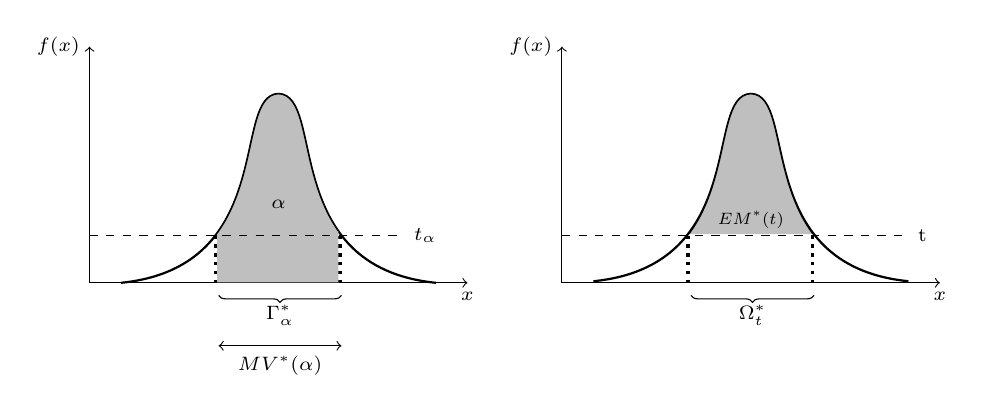
\begin{tikzpicture}[scale=2.]

\draw[->](7.8,0)--(10.2,0) node[below]{\scriptsize $x$};
\draw[->](7.8,0)--(7.8,1.5) node[left]{\scriptsize $f(x)$}; 
\draw [thick] (8,0) ..controls +(1,0.1) and +(-0.3,-0.01).. (9,1.2);
\draw [thick] (9,1.2) ..controls +(0.3,-0.01) and +(-1,0.1).. (10,0);

\draw[dotted,very thick](8.60,0.3)--(8.60,0) node[right]{};
\draw[dotted,very thick](9.39,0.3)--(9.39,0) node[right]{};

%\draw (8,0.3)--(10,0.3)--(10,1.5)--(8,1.5)--(8,0.3); dessine 4 segments correspondant au 4 points

%hachurage :
\begin{scope} 
\clip (8.61,0)--(9.38,0)--(9.38,1.5)--(8.61,1.5)--(8.61,0) ; %tout ce qui est dans begin{scope} se limitera au rectangle

\path[draw,fill=lightgray] (8,0) ..controls +(1,0.1) and +(-0.3,-0.01).. (9,1.2)--
(9,1.2) ..controls +(0.3,-0.01) and +(-1,0.1).. (10,0)--
(8,0)--(10,0) --cycle;
\end{scope}

\draw[dashed](7.8,0.3)--(9.8,0.3) node[right]{\scriptsize $t_\alpha$};

%accolade :
\draw[decorate,decoration={brace}]
(9.4,-0.08)--(8.62,-0.08) node[below,pos=0.5] {\scriptsize $\Gamma_\alpha^*$};

\draw[<->]
(9.4,-0.4)--(8.62,-0.4) node[below,pos=0.5] {\scriptsize $MV^*(\alpha)$};



\draw (9,0.5) node[thick]{\scriptsize $\alpha$} ;
%\draw (8.8,-0.8) node[thick]{Figure 1: MV curve} ;

\draw[->](10.8,0)--(13.2,0) node[below]{\scriptsize $x$};
\draw[->](10.8,0)--(10.8,1.5) node[left]{\scriptsize $f(x)$}; 
\draw [thick] (11,0.01) ..controls +(1,0.1) and +(-0.3,-0.01).. (12,1.2);
\draw [thick] (12,1.2) ..controls +(0.3,-0.01) and +(-1,0.1).. (13,0.01);
\draw[dashed](10.8,0.3)--(13,0.3) node[right]{\scriptsize t};
\draw[dotted,very thick](11.60,0.3)--(11.60,0) node[right]{};
\draw[dotted,very thick](12.39,0.3)--(12.39,0) node[right]{};

%\draw (8,0.3)--(10,0.3)--(10,1.5)--(8,1.5)--(8,0.3); dessine 4 segments correspondant au 4 points

%hachurage :
\begin{scope} 
\clip (11,0.31)--(13,0.308)--(13,1.5)--(11,1.5)--(11,0.308) ; %tout ce qui est dans begin{scope} se limitera au rectangle (8,0.3)--(10,0.3)--(10,1.5)--(8,1.5)--(8,0.3)
\path[draw,fill=lightgray] (11,0) ..controls +(1,0.1) and +(-0.3,-0.01).. (12,1.2)--
(12,1.2) ..controls +(0.3,-0.01) and +(-1,0.1).. (13,0)--
(11,0.3)--(13,0.3) --cycle;
\end{scope}

%accolade :
\draw[decorate,decoration={brace}]
(12.4,-0.08)--(11.62,-0.08) node[below,pos=0.5] {\scriptsize  $\Omega_t^*$};

\draw (12,0.4) node[scale=0.85]{\scriptsize $EM^*(t)$} ;
\draw (11.8,-0.5) node[thick]{ } ;
\end{tikzpicture}
}
\end{figure}
\end{center}

\subsection{Numerical unsupervised criteria}

The main advantage of EM compared to MV is that the area under its curve is finite, even if the support of the distribution $F$ is not.
As curves cannot be trivially compared, consider the $L^1$-norm $\|.\|_{L^1(I)}$ with $I\subset \rset$ an interval. As $MV^*=MV_f$ is below $MV_s$ point-wise, $\argmin_s \| MV_s - MV^* \|_{L^1(I)} = \argmin \| MV_s \|_{L^1(I)} $. We thus define the criterion
$\crit^{MV}(s) = \| MV_s \|_{L^1(I^{MV})},$ which is equivalent to consider $\| MV_s - MV^* \|_{L^1(I^{MV})}$ as mentioned in the introduction. As we are interested in evaluating accuracy on large density level-sets, one natural interval $I^{MV}$ would be for instance $[0.9, 1]$. However, MV diverges at one when the support is infinite, so that we arbitrarily take $I^{MV} = [0.9, 0.999].$
The smaller is $\crit^{MV}(s)$, the better is the scoring function $s$.
%
Similarly, we consider $\crit^{EM}(s) = \| EM_s \|_{L^1(I^{EM})}, $ this time considering $I^{EM} = [0,EM^{-1}(0.9)],$ with $EM_s^{-1}(0.9) := \inf\{t\ge 0,~ EM_s(t) \le 0.9\}$, as $EM_s(0)$ is finite (equal to $1$). We point out that such small values of $t$ correspond to large level-sets. Also, we have observed that
$EM_s^{-1}(0.9)$ (as well as $EM_f^{-1}(0.9)$) varies significantly depending on the dataset. Generally, for datasets in large dimension, it can be % $\widehat{EM}_s^{-1}(0.9)$ is
very small (in the experiments, smallest values are of order $10^{-7}$) as it is of the same order of magnitude as the inverse of the total support volume.
% , and are not comparable between scoring function (that is why $[0, 0.1]$ has not be chosen for $I$). Another possibility would have been to take $I = [0,t^s_{0.9}]$ with $t^s_{0.9} := \sup_{t\ge 0} \mathbb{P}(s(X) > t) \ge 0.9$.

As the distribution $F$ of the normal data is generally unknown, mass-volume and excess-mass curves must be estimated. Let $s\in \mathcal{S}$ and $\mb X_1,\; \ldots,\; \mb X_n$ be an i.i.d. sample with common distribution $F$ and set $$\mathbb{P}_n(s \ge t)=\frac{1}{n}\sum_{i=1}^n\mathds{1}_{s(\mb X_i)\geq t}.$$ The empirical MV and EM curves of $s$ are then simply defined as empirical version of \eqref{evaluation:MV-def} and \eqref{evaluation:EM-def}, 
\begin{align}
\label{evaluation:MV-def-emp}
\widehat{MV}_s(\alpha) &= \inf_{u \ge 0} \leb(s \ge u) ~~~~\st~~~~ \mathbb{P}_n(s \ge u) \ge \alpha\\
\label{evaluation:EM-def-emp}
\widehat{EM}_s(t) &= \sup_{u \ge 0} \mathbb{P}_n(s \ge u) ~-~ t \leb(s \ge u)
%\lambda_s \circ \alpha_s^{-1}(\alpha),
\end{align}
%
Note that in practice, the volume $\leb(s \ge u)$ is estimated using Monte-Carlo approximation, which only applies to small dimensions.
%
Finally, we obtain the empirical EM and MV based performance criteria:
\begin{align}
\label{evaluation:eq:standard_emp_EM}\widehat{\crit}^{EM}(s) &= \| \widehat{EM}_s \|_{L^1(I^{EM})}  &&I^{EM} = [0,\widehat{EM}^{-1}(0.9)],\\
\label{evaluation:eq:standard_emp_MV}\widehat{\crit}^{MV}(s) &= \| \widehat{MV}_s \|_{L^1(I^{MV})}  &&I^{MV} = [0.9, 0.999],
\end{align}

\begin{remark}({\sc Link with ROC curve})
To evaluate unsupervised algorithms, it is common to generate uniform outliers and then use the ROC curve approach. Up to identify the Lebesgue measure of a set to its empirical version (\ie~the proportion of uniform point inside),
this approach is equivalent to using the mass-volume curve \citep{CLEM14}.
 However, in the former approach, the volume estimation does not appear directly, so that the (potentially huge) amount of uniform points needed to provide a good estimate of a volume is often not respected, yielding optimistic performances.
\end{remark}
\section{Scaling with dimension}
\label{evaluation:scaling-dim}
In this section we propose a methodology to scale the use of the excess-mass and mass-volume criteria to large dimensional data. It consists in sub-sampling training \emph{and} testing data along features, thanks to a parameter $d'$ controlling the number of features randomly chosen for computing the (EM or MV) score. Replacement is done after each draw of features $F_1,\ldots,F_{m}$. A partial score $\widehat \crit_k^{MV}$ (resp. $\widehat \crit_k^{EM}$) is computed for each draw $F_k$ using \eqref{evaluation:eq:standard_emp_EM} (resp. \eqref{evaluation:eq:standard_emp_MV}). The final performance criteria are obtained by averaging these partial criteria along the different draws of features. This methodology is described in Algorithm~\ref{evaluation:algo:EMMV}.
%
% \begin{align}
% \label{evaluation:MV_high}
% \widehat{\crit}^{MV}_{high\_dim} &= \frac{1}{m} \sum_{k=1}^{m}\widehat \crit_{F_k}^{MV}\\
% \label{evaluation:EM_high}
% \widehat{\crit}^{EM}_{high\_dim} &= \frac{1}{m} \sum_{k=1}^{m}\widehat \crit_{F_k}^{EM}
% \end{align}
%
\begin{algorithm}[!tbh]
\caption{~~Evaluate anomaly detection algorithms on high dimensional data}
\label{evaluation:algo:EMMV}
\begin{algorithmic}
  \STATE \textbf{Inputs}: anomaly detection algorithm $\mathcal{A}$, data set $X = (x^j_i)_{1 \le i \le n, 1 \le j \le d }$, feature sub-sampling size $d'$, number of draws $m$.\\~\\
%  \STATE{Randomly split $S_n$ into a training set $S_{train}$ and a test set $S_{test}$}

  \FOR{$k=1,\ldots,m$}
    \STATE{randomly select a sub-group $F_k$ of $d'$ features}
    \STATE{compute the associated scoring function $\widehat s_{k} = \mathcal{A}\big((x^j_i)_{1 \le i \le n,~j \in F_k}\big)$}
    \STATE compute $\widehat{\crit}_k^{EM} = \| \widehat{EM}_{\widehat s_k} \|_{L^1(I^{EM})}$ using \eqref{evaluation:eq:standard_emp_EM} or $\widehat{\crit}_k^{MV} = \| \widehat{MV}_{\widehat s_k} \|_{L^1(I^{MV})}$ using \eqref{evaluation:eq:standard_emp_MV}
    % \FOR{$\beta$ in $\Bigl\{\alpha_1 + j\frac{\alpha_2 -\alpha_1}{n_{\alpha}-1}, j \in \{0, \dots, n_{\alpha}-1 \} \Bigr\}$}
    %   \STATE Find $\hat \rho_{\beta}$ such that
    %   \begin{equation*}
    %   P_{test}(\widehat \Omega_{\beta}) = \beta
    %   \end{equation*}
    %   where $\widehat \Omega_{\beta} = \{x, \hat s_{\theta}(x) \geq \hat \rho_{\beta}\}$
    %   \STATE Computation of the volume $\lambda_{\hat s_{\theta}} = \lambda(\widehat \Omega_{\beta})$
    % \ENDFOR
    % \STATE Compute Area under the estimated Mass Volume curve over $I = [\alpha_1, \alpha_2]$: $\text{AMV}^{test}_I(\hat s_{\theta})$
  \ENDFOR \\~\\

  \STATE \textbf{Return} performance criteria: $$\widehat{\crit}^{EM}_{high\_dim} (\mathcal{A})= \frac{1}{m} \sum_{k=1}^m\widehat \crit_k^{EM} \text{~~~~or~~~~} \widehat{\crit}^{MV}_{high\_dim}(\mathcal{A}) = \frac{1}{m} \sum_{k=1}^m\widehat \crit_k^{MV}~.$$
\end{algorithmic}
\end{algorithm}
%

A drawback from this approach is that we do not evaluate combinations of more than $d'$ features within the dependence structure. However, according to our experiments, this is enough in most of the cases. Besides, we solve two major drawbacks inherent to mass-volume or excess-mass criteria, % (as explained in the previous section)
which come from the Lebesgue reference measure:
\begin{itemize}
\item  EM or MV performance criteria cannot be estimated in large dimension,
\item  EM or MV performance criteria cannot be compared when produced from spaces of different dimensions, since reference measures of $\mathbb{R}^d$ and $\mathbb{R}^{d+1}$ cannot be compared.
\end{itemize}

\begin{remark}({\sc Feature Importances})
With standard MV and EM curves, the benefit of using or not some feature $j$ in training \emph{cannot} be evaluated, as it involves spaces of different dimensions ($d$ and $d+1$). % (as noticed above, reference measures of $\mathbb{R}^d$ and $\mathbb{R}^{d+1}$ cannot be compared).
%
Solving the second drawback precisely allows to evaluate the importance of features.
% , so that our criteria cannot be compared. 
By sub-sampling features, we can compare accuracies with or without using feature $j$: when computing $\widehat{\crit}^{MV}_{high\_dim}$ or $\widehat{\crit}^{EM}_{high\_dim}$ using Algorithm~\ref{evaluation:algo:EMMV}, this is reflected in the fact that $j$ can (resp. cannot) be drawn.
\end{remark}

\begin{remark}({\sc Theoretical Grounds})
Criteria $\widehat{\crit}^{MV}_{high\_dim}$ or $\widehat{\crit}^{EM}_{high\_dim}$ do not evaluate a specific scoring function $s$ produced by some algorithm (on some dataset), but the algorithm itself \wrt~the dataset at stake. Indeed, these criteria proceed with the average of partial scoring functions on sub-space of $\mathbb{R}^d$. We have no theoretical guaranties that the final score does correspond to some scoring function defined on $\mathbb{R}^d$. In this work, we only show that from a practical point of view, it is a useful and accurate methodology to compare algorithms performance on large dimensional datasets.
\end{remark}

\begin{remark}({\sc default parameters}) 
In our experiments, we arbitrarily chose $m = 50$ and $d'=5$. This means that $50$ draws of $5$ features (with replacement after each draw) have been done. Volume in spaces of dimension $5$ have thus to be estimated (which is feasible with Monte-Carlo), and $50$ scoring functions (on random subspaces of dimension $5$) have to be computed by the algorithm we want to evaluate.
The next section shows (empirically) that these parameters achieve a good accuracy on the collection of datasets studied, the largest dimension considered being $164$.
\end{remark}

\section{Benchmarks}
\label{evaluation:sec:benchmarks}

\textbf{Does performance in term of EM/MV correspond to performance in term of ROC/PR?} Can we recover, on some fixed dataset, which algorithm is better than the others (according to ROC/PR criteria) without using labels?
In this section we study four different empirical evaluations (ROC, PR, EM, MV) of three classical state-of-the-art anomaly detection algorithms, One-Class SVM  \citep{Scholkopf2001}, Isolation Forest \citep{Liu2008}, and Local Outlier Factor (LOF) algorithm \citep{Breunig2000LOF}, on 12 well-known anomaly detection datasets. Two criteria use labels (ROC and PR based criteria) and two do not (EM and MV based criteria).
% To evaluate accuracy, we compare two criteria using the data labels (ROC and PR curves), and the two unsupervised criteria (Excess-Mass and Mass-Volume curves).
% More specifically, we use the area under the curves as numerical criterion.
For ROC and PR curves, we consider the area under the (full) curve (AUC). For the excess-mass curve $EM(t)$ (resp. mass-volume curve), we consider the area under the curve on the interval $[0, EM^{-1}(0.9)]$ (resp. $[0.9, 0.999]$) as described in Section~\ref{evaluation:background}.

\subsection{Datasets description}

\begin{table}[!ht]
\caption{Original Datasets characteristics}
\label{evaluation:table:data}
\centering
%\tabcolsep=0.2cm
\resizebox{\linewidth}{!} {
\begin{tabular}{l cc ll }
  \toprule
  ~           & nb of samples      & nb of features     & ~~~~~~~~~~~~~~~~~~~~~~~~~anomaly class      & ~                  \\ \cmidrule{1-5}
  adult       & 48842              & 6                  &    class '$>50K$'                           &      (23.9\%)      \\
  http        & 567498             & 3                  &      attack                                 &    (0.39\%)        \\
  pima        & 768                & 8                  &    pos (class 1)                            &        (34.9\%)    \\
  smtp        & 95156              & 3                  &      attack                                 &    (0.03\%)        \\
  wilt        & 4839               & 5                  &    class 'w' (diseased trees)               &    (5.39\%)        \\
  annthyroid  & 7200               & 6                  &    classes $\neq$ 3                         &        (7.42\%)    \\
  arrhythmia  & 452                & 164                &    classes $\neq$ 1 (features 10-14 removed)&  (45.8\%)          \\
  forestcover & 286048             & 10                 &    class 4  (vs. class 2 )                  &           (0.96\%) \\
  ionosphere  & 351                & 32                 &    bad                                      &       (35.9\%)     \\
  pendigits   & 10992              & 16                 &    class 4                                  &        (10.4\%)    \\
  shuttle     & 85849              & 9                  &      classes $\neq$ 1 (class 4 removed)     &  (7.17\%)          \\
  spambase    & 4601               & 57                 &    spam                                     &           (39.4\%) \\
  \bottomrule
\end{tabular}
}
\end{table}

%  since only large level sets % (containing at least $90\%$ of the data)
% are of interest to evaluate anomaly detection algorithms accuracy.
% For the same reason and as previously described, we also restrict our attention to the interval $[0.9, 0.999]$ concerning the mass-volume curve $MV(\alpha)$ (the mass-volume curve potentially diverges when $\alpha \to 1$).% Note that we do not consider $[0.9, 1]$ since the mass-volume curve potentially diverges when $\alpha \to 1$, so that the area is infinite.


% Point out that standards excess-mass and mass-volume scores refer on the Lebesgue measure, and thus require volume estimation. Hence, they only apply to continuous datasets.

The characteristics of these reference datasets are summarized in Table~\ref{evaluation:table:data}. They are all available on the UCI repository \citep{Lichman2013} and the preprocessing is done in a classical way. %, excepting for the \emph{adult} dataset. For the latter, we considered the 6 continuous features.
We removed all non-continuous attributes as well as attributes taking less than $10$ different values.
%
The \emph{http} and \emph{smtp} datasets belong to the KDD Cup '99 dataset \citep{KDD99,Tavallaee2009}, which consists of a wide variety of hand-injected  attacks (anomalies) in a closed network (normal background). They are classically obtained as described in \cite{Yamanishi2000}. These datasets are available on the \emph{scikit-learn} library \citep{sklearn2011}.
The \emph{shuttle} dataset is the fusion of the training and testing datasets available in the UCI repository. As in \cite{Liu2008}, we use instances from all different classes but class $4$. %, which yields an anomaly ratio (class 1) of $7.17\%$.
In the \emph{forestcover} data, the normal data are the instances from class~$2$ while instances from class $4$ are anomalies (as in \cite{Liu2008}). %, which yields an anomaly ratio of $0.9\%$. 
The \emph{ionosphere} dataset differentiates `good' from `bad' radars, considered here as abnormal. A `good' radar shows evidence of some type of structure in the ionosphere. A `bad' radar does not, its signal passing through the ionosphere.
The \emph{spambase} dataset consists of spam or non-spam emails. The former constitute the abnormal class.
The \emph{annthyroid} medical dataset on hypothyroidism contains one normal class and two abnormal ones, which form the outlier set.
The \emph{arrhythmia} dataset reflects the presence and absence (class $1$) of cardiac arrhythmia. The number of attributes being large considering the sample size, we removed attributes containing missing data.
The \emph{pendigits} dataset contains 10 classes corresponding to the digits from 0 to 9, examples being handwriting samples. As in \cite{Schubert2012}, the abnormal data are chosen to be those from class 4.
The \emph{pima} dataset consists of medical data on diabetes. Patients suffering from diabetes (positive class) were considered outliers.
The \emph{wild} dataset involves detecting diseased trees in Quickbird imagery. Diseased trees (class `w') is the abnormal class.
In the \emph{adult} dataset, the goal is to predict whether income exceeds \$ 50K/year based on census data. Only the 6 continuous attributes are kept.

\subsection{Results}

The experiments are performed both in a novelty detection framework (also named semi-supervised framework, the training set consisting of normal data only) and in an unsupervised framework (the training set is polluted by abnormal data).
In the former case, we simply removed anomalies from the training data, and EM and PR criteria are estimated using only normal data.
In the latter case, the anomaly rate is arbitrarily bounded to $10\%$ max, and EM and PR criteria are estimated with the same test data used for ROC and PR curves, without using their labels.

\begin{table}[!ht]
\centering
\caption{Results for the novelty detection setting. ROC, PR, EM, MV often do agree on which algorithm is the best (in bold), which algorithm is the worse (underlined) on some fixed datasets. When they do not agree, it is often because ROC and PR themselves do not, meaning that the ranking is not clear.}
\label{evaluation:table:results-semisupervised}
\footnotesize
\tabcolsep=0.11cm
\resizebox{\linewidth}{!} {
\begin{tabular}{l cccc c cccc c cccc}
\toprule
Dataset      & \multicolumn{4}{c}{iForest}& & \multicolumn{4}{c}{OCSVM}&  & \multicolumn{4}{c}{LOF} \\ %& parameters $(\epsilon, k)$\\
  \cmidrule{1-15}

~            & ROC  & PR   & EM    &  MV  &  & ROC  & PR   & EM    & MV     &  & ROC  & PR   & EM    & MV    \\
adult        &\bf 0.661 &\bf 0.277 &\bf 1.0e-04&\bf 7.5e01&  &0.642 &0.206 &2.9e-05& 4.3e02 &  &\underline{0.618} &\underline{0.187}&\underline{1.7e-05}&\underline{9.0e02} \\
http         &0.994 &0.192 &1.3e-03&9.0   &  &\bf 0.999 &\bf 0.970 &\bf 6.0e-03&\bf 2.6  &     &\underline{0.946} &\underline{0.035} &\underline{8.0e-05}&\underline{3.9e02} \\
pima         &0.727 &0.182 &5.0e-07&\bf 1.2e04&  &\bf 0.760 &\bf 0.229 &\bf 5.2e-07&\underline{1.3e04} &   &\underline{0.705} &\underline{0.155} &\underline{3.2e-07}&2.1e04 \\
smtp         &0.907 &\underline{0.005} &\underline{1.8e-04}&\underline{9.4e01}&  &\underline{0.852} &\bf 0.522 &\bf 1.2e-03&8.2    &   &\bf 0.922 &0.189 & 1.1e-03&\bf 5.8    \\
wilt         &0.491 &0.045 &4.7e-05&\underline{2.1e03} & &\underline{0.325} &\underline{0.037} &\bf 5.9e-05&\bf 4.5e02 &   &\bf 0.698 &\bf 0.088 &\underline{2.1e-05}&1.6e03 \\ 
 &&&&&&&&&&&&&& \\
% internet\_ads&0.414 &0.109 &  NA   &  NA    &      &      &       &          &0.540 &0.139 &       &       \\
% SA           &0.988 &0.386 &  NA   &  NA    &      &      &       &          &0.880 &0.018 &       &       \\
% SF           &0.936 &0.038 &  NA   &  NA    &      &      &       &          &0.891 &0.022 &       &       \\
annthyroid   &\bf 0.913 &\bf 0.456 &\bf 2.0e-04&2.6e02 & &\underline{0.699} &\underline{0.237} &\underline{6.3e-05}&\bf 2.2e02 &   &0.823 &0.432 &6.3e-05&\underline{1.5e03} \\
arrhythmia   &\bf 0.763 &\bf 0.487 &\bf 1.6e-04&\bf 9.4e01 & &0.736 &0.449 &1.1e-04&1.0e02   & &\underline{0.730} &\underline{0.413} &\underline{8.3e-05}&\underline{1.6e02} \\
forestcov.   &\underline{0.863} &\underline{0.046} &\underline{3.9e-05}&\underline{2.0e02}&  &0.958 &0.110 &5.2e-05&1.2e02  &  &\bf 0.990 &\bf 0.792 &\bf 3.5e-04&\bf 3.9e01 \\
ionosphere   &\underline{0.902} &\underline{0.529} &\underline{9.6e-05}&\underline{7.5e01} & &\bf 0.977 &\bf 0.898 &\bf 1.3e-04&\bf 5.4e01  &  &0.971 &0.895 &1.0e-04&7.0e01 \\
pendigits    &0.811 &0.197 &2.8e-04&2.6e01 & &\underline{0.606} &\underline{0.112} &\underline{2.7e-04}&\underline{2.7e01}   & &\bf 0.983 &\bf 0.829 &\bf 4.6e-04&\bf 1.7e01 \\
shuttle      &0.996 &0.973 &1.8e-05&5.7e03 & &\underline{0.992} &\underline{0.924} &\bf 3.2e-05&\bf 2.0e01   & &\bf 0.999 &\bf 0.994 &\underline{7.9e-06}&\underline{2.0e06} \\
spambase     &\bf 0.824 &\bf 0.371 &\bf 9.5e-04&\bf 4.5e01&  &\underline{0.729} &0.230 &4.9e-04&1.1e03  &  &0.754 &\underline{0.173} &\underline{2.2e-04}&\underline{4.1e04} \\
\bottomrule
\end{tabular}
}
\end{table}

Recall that standard excess-mass and mass-volume performance criteria referring on the Lebesgue measure, they require volume estimation. They only apply to continuous datasets, of small dimension ($d \le 8$). The datasets verifying these requirements are \emph{http}, \emph{smtp}, % \emph{shuttle}, \emph{pendigits},
\emph{pima}, \emph{wilt} and \emph{adult}.
For the other datasets, we use the performance criteria $\widehat{\crit}^{MV}_{high\_dim}$ and $\widehat{\crit}^{EM}_{high\_dim}$ computed with Algorithm~\ref{evaluation:algo:EMMV}. We arbitrarily chose $m = 50$ and $d'=5$, which means that $50$ draws of $5$ features, with replacement after each draw, are done.
Other parameters have also been tested but are not presented here. The default parameters proposed here are a compromise between computational time and performance, in particular on the largest dimensional datasets. The latter require a relatively large product $m \times d'$, which is the maximal number of different features that can be drawn.


\begin{table}[!ht]
\centering
\caption{Results for the unsupervised setting still remain good: one can see that ROC, PR, EM, MV often do agree on which algorithm is the best (in bold), which algorithm is the worse (underlined) on some fixed datasets. When they do not agree, it is often because ROC and PR themselves do not, meaning that the ranking is not clear.}
\label{evaluation:table:results-unsupervised}
\footnotesize
\tabcolsep=0.11cm
\resizebox{\linewidth}{!} {
\begin{tabular}{l cccc c cccc c cccc}
\toprule
Dataset      & \multicolumn{4}{c}{iForest} & & \multicolumn{4}{c}{OCSVM} & & \multicolumn{4}{c}{LOF} \\ %& parameters $(\epsilon, k)$\\
  \cmidrule{1-15}
~            & ROC  & PR   & EM    &  MV  &  & ROC   & PR    & EM    & MV    &    & ROC  & PR   & EM    & MV    \\
adult        &\bf 0.644 &\bf 0.234 &\bf 6.6e-05&\bf 2.7e02 & &0.627  &0.184  &1.8e-05&5.6e02   &  &\underline{0.545} &\underline{0.098} &\underline{7.4e-06}&\underline{1.9e03} \\
http         &\bf 0.999 &\bf 0.686 &1.4e-03&2.2e01&  &0.994  &0.207  &\bf 5.7e-03&\bf 3.3    &    &\underline{0.354} &\underline{0.019} &\underline{9.8e-05}&\underline{3.9e02} \\
pima         &\bf 0.747 &0.205 &\bf 1.2e-06&\bf 1.2e04 & &0.742  &\bf 0.211  &6.0e-07&1.9e04  &   &\underline{0.686} &\underline{0.143} &\underline{6.0e-07}&\underline{3.2e04} \\
smtp         &0.902 &\underline{0.004} &\underline{2.7e-04}&\underline{8.6e01}&  &\underline{0.852}  &\bf 0.365  &\bf 1.4e-03&7.7   &     &\bf 0.912 &0.057 &1.1e-03&\bf 7.0    \\ %XXX weird MV != EM
wilt         &0.443 &0.044 &3.7e-05&\underline{2.2e03} & &\underline{0.318}  &\underline{0.036}  &\bf 3.9e-05&\bf 4.3e02 &    &\bf 0.620 &\bf 0.066 &\underline{2.0e-05}&8.9e02 \\  &&&&&&&&&&&&&& \\

% internet\_ads&0.693 &0.359 &  NA   &  NA    &       &       &       &           &0.446 &0.119 &       &       \\
% SA           &0.995 &0.526 &  NA   &  NA    &       &       &       &           &0.780 &0.026 &       &       \\
% SF           &0.964 &0.067 &  NA   &        &       &       &       &           &0.465 &0.007 &       &       \\
annthyroid   &\bf 0.820 &\bf 0.309 &\bf 6.9e-05&7.7e02 & &\underline{0.682}  &0.187  &4.1e-05&\bf 3.1e02  &   &0.724 &\underline{0.175} &\underline{1.6e-05}&\underline{4.1e03} \\
arrhythmia   &\bf 0.740 &0.416 &\bf 8.4e-05&\bf 1.1e02 & &0.729  &\bf 0.447  &6.8e-05&1.2e02   &  &\underline{0.729} &\underline{0.409} &\underline{5.6e-05}&\underline{1.5e02} \\
forestcov.   &0.882 &0.062 &\underline{3.2e-05}&\underline{2.3e02} & &\bf 0.951  &\bf 0.095  &4.4e-05&1.4e02    & &\underline{0.542} &\underline{0.016} &\bf 2.4e-04 &\bf 4.6e01 \\
ionosphere   &\underline{0.895} &\underline{0.543} &7.4e-05&\underline{9.3e01} & &\bf 0.977  &\bf 0.903  &\bf 8.7e-05&\bf 7.7e01   &  &0.969 &0.884 &\underline{6.9e-05}&1.0e02 \\
pendigits    &0.463 &0.077 &2.7e-04&2.5e01 & &\underline{0.366}  &\underline{0.067}  &\underline{2.6e-04}&\underline{2.8e01}&   &\bf 0.504 &\bf 0.089 &\bf 4.5e-04&\bf 1.6e01 \\
shuttle      &\bf 0.997 &\bf 0.979 &7.1e-07&1.2e05 & &0.992  &0.904  &\bf 5.8e-06&\bf 1.7e02  &   &\underline{0.526} &\underline{0.116} &\underline{7.1e-07}&\underline{1.7e07} \\
spambase     &\bf 0.799 &\bf 0.303 &\bf 2.2e-04&\bf 3.5e01 & &0.714  &0.214  &1.5e-04&2.9e02  &   &\underline{0.670} &\underline{0.129} &\underline{3.7e-05}&\underline{2.7e04} \\
\bottomrule
\end{tabular}
}
\end{table}





Excess-Mass, Mass-volume, ROC and Precision-Recall curves AUCs are presented in Table~\ref{evaluation:table:results-semisupervised} for the novelty detection framework, and in Table~\ref{evaluation:table:results-unsupervised} for the unsupervised framework. The corresponding ROC and PR curves are available at the end of this chapter. %for Isolation Forest are plotted in Figures~\ref{evaluation:fig:iforest_roc_pr}, for the unsupervised setting. The ROC and PR curves for the unsupervised setting are available in supplementary material, as well as the ROC and PR curves of LOF and OCSVM.
 % \ref{evaluation:fig:ocsvm_roc_pr} and \ref{evaluation:fig:lof_roc_pr} for the semi-supervised framework (resp. \ref{evaluation:fig:iforest_roc_pr_unsupervised}, \ref{evaluation:fig:ocsvm_roc_pr_unsupervised} and \ref{evaluation:fig:lof_roc_pr_unsupervised} for the unsupervised setup).
%
Figure~\ref{evaluation:mv_em_adult} shows excess-mass and mass-volume curves on the adult dataset in a novelty detection setting. %, which is more than $75\%$ of good comparisons with respect to both ROC and PR scores
Corresponding figures for the other datasets are also available at the end of this chapter.

\begin{figure}[!ht]
  \centering
  \caption{MV and EM curves for adult dataset (novelty detection framework). Both in terms of EM and MV curves, iForest is found to perform better than OCSVM, which is itself found to perform better than LOF. Comparing to Table~\ref{evaluation:table:results-semisupervised}, ROC and PR AUCs give the same ranking (iForest on adult $\succ$ OCSVM on adult $\succ$ LOF on adult). The 3 pairwise comparisons (iForest on adult, LOF on adult), (OCSVM on adult, LOF on adult) and (OCSVM on adult, iForest on adult) are then similarly ordered by EM, PR, MV and EM criteria.}
  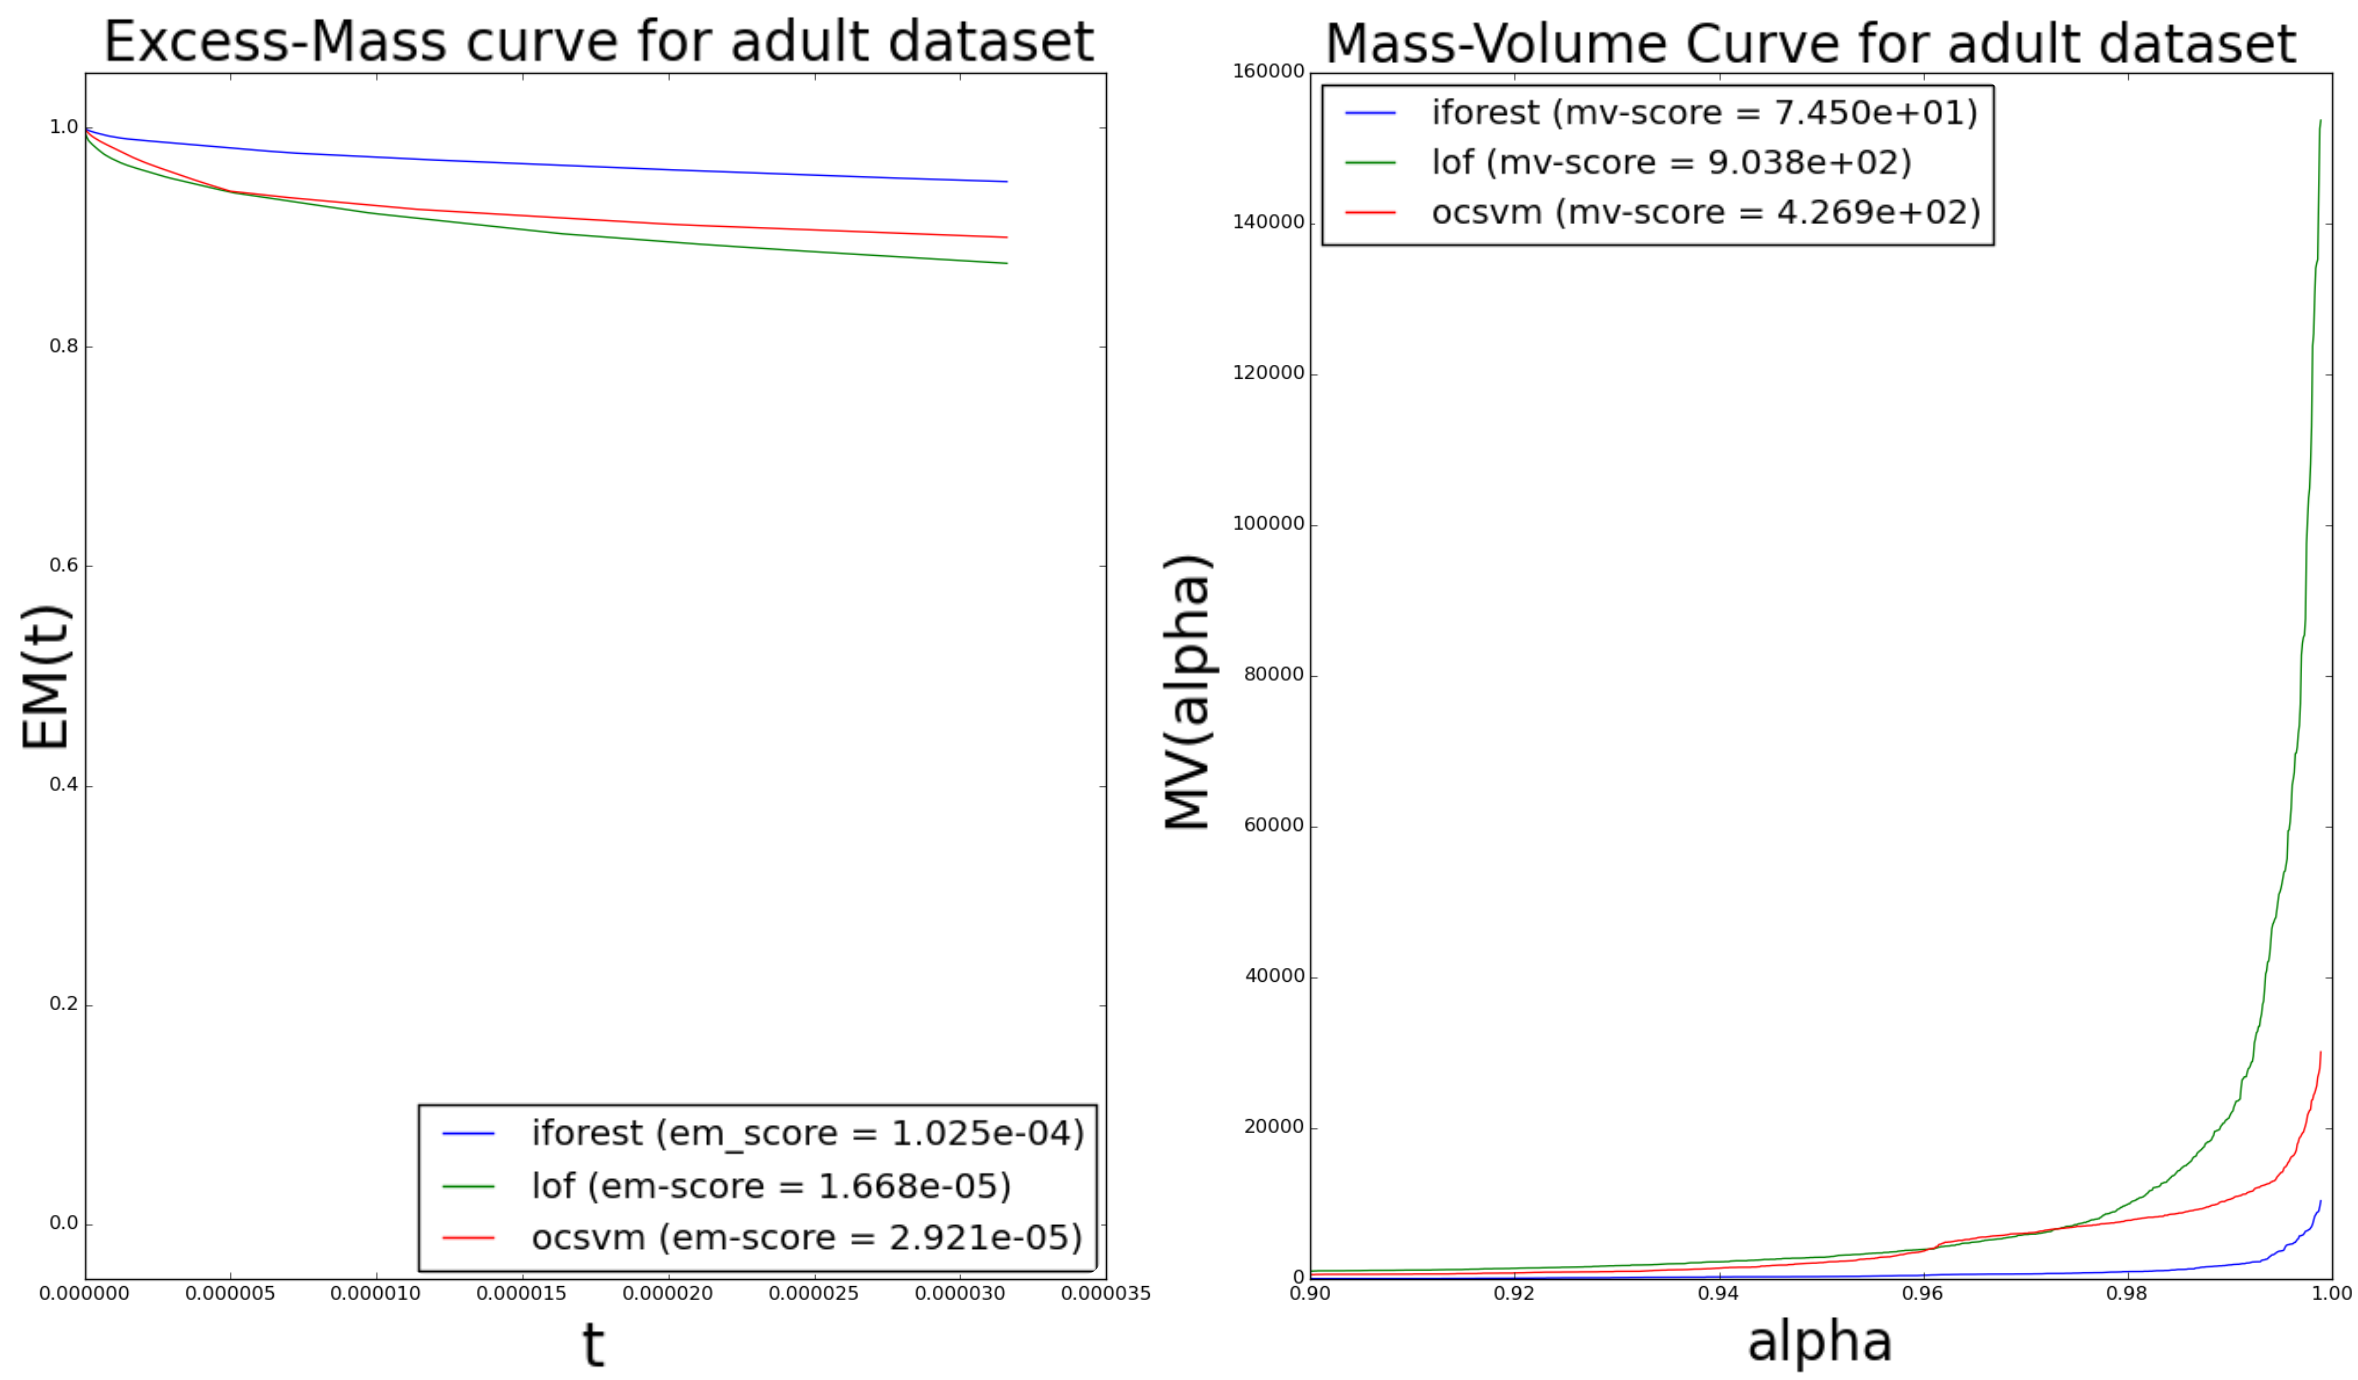
\includegraphics[width=\linewidth]{fig_source/evaluation_fig/mv_em_adult_supervised_09_factorized_inkscape.png}
\label{evaluation:mv_em_adult}
\end{figure}

Results from Table~\ref{evaluation:table:results-semisupervised} can be summarized as follows. Consider the $36$ possible pairwise comparisons between the three algorithms over the twelve datasets
\begin{align}
\label{evaluation:eq:pairs}
\bigg\{\Big(A_1 \text{~on~} \mathcal{D}, A_2 \text{~on~} \mathcal{D}\Big),~~ A_1, A_2 \in \{\text{iForest, LOF, OCSVM}\},~~ \mathcal{D} \in \{\text{adult, http, \ldots, spambase}\} \bigg\}.
\end{align}
%
For each dataset $\mathcal{D}$, there are three possible pairs (iForest on $\mathcal{D}$, LOF on $\mathcal{D}$), (OCSVM on $\mathcal{D}$, LOF on $\mathcal{D}$) and (OCSVM on $\mathcal{D}$, iForest on $\mathcal{D}$).
%
Then the EM-score discriminates $28$ of them ($78\%$) as ROC score does, and $29$ ($81\%$) of them as PR score does. 
Intuitively this can be interpreted as follows. Choose randomly a dataset $\mathcal{D}$ among the twelve available, and two algorithms $A_1$, $A_2$ among the three available. This amounts to choose at random a pairwise comparison ($A_1$ on $\mathcal{D}$, $A_2$ on $\mathcal{D}$) among the $36$ available. Suppose that according to ROC criterion, $A_1$ is better than $A_2$ on dataset $\mathcal{D}$, \ie~($A_1$ on $\mathcal{D}$) $\succ$ ($A_2$ on $\mathcal{D}$). Then the EM-score discriminates $A_1$ and $A_2$ on dataset $\mathcal{D}$ in the same way, \ie~also finds $A_1$ to be better than $A_2$ on dataset $\mathcal{D}$ with $78$ percent chance.

 Besides, let us consider pairs ($A_1$ on $\mathcal{D}$, $A_2$ on $\mathcal{D}$) which are
similarly ordered by ROC and PR criteria, namely \st~ $A_1$ is better than $A_2$ (or the reverse) on dataset $\mathcal{D}$ according to both EM and PR. According to Table~\ref{evaluation:table:results-semisupervised}, this represents every pairs but one in \emph{spambase} and two in \emph{smtp}. Then, one achieves $27/33 = 82\%$ of similarly discriminated pairs (\wrt~to ROC and PR criteria). Moreover, EM is able to recover the exact (\wrt~ROC and PR criteria) ranking of ($A_1$ on $\mathcal{D}$, $A_2$ on $\mathcal{D}$, $A_3$ on $\mathcal{D}$) on every datasets $\mathcal{D}$ excepting \emph{wilt} and \emph{shuttle}. For \emph{shuttle}, note that ROC scores are very close to each other ($0.996$, $0.992$, $0.999$) and thus not clearly discriminates algorithms. The only significant error committed by EM is for the \emph{wilt} dataset (on which no feature sub-sampling is done due to the low dimension). This may come from anomalies not being far enough in the tail of the normal distribution, \eg~forming a cluster near the support of the latter distribution. %Experiments with feature sub-sampling (as for larger dimensional datasets) have not shown any improvement. 

Same conclusions and similar accuracies hold for MV-score, which only makes one additional error on the pair (iForest on $pima$, OCSVM on $pima$).
%
Considering all the 36 pairs \eqref{evaluation:eq:pairs}, % ($A_1$ on $\mathcal{D}$, $A_2$ on $\mathcal{D}$), $A_1, A_2 \in \{\text{iForest, LOF, OCSVM}\}$, $\mathcal{D}$ one of the twelve datasets
one observes $75\%$ of good comparisons \wrt~ROC-score, and $72\%$ \wrt~PR score.
Considering the pairs which are similarly ordered by ROC and PR criteria, this rate increases to $25/33 = 76\%$. The errors are essentially made on \emph{shuttle}, \emph{wild} and \emph{annthyroid} datasets. 

Results from the unsupervised framework (training and testing data are polluted by outliers) are similar for both EM and MV criteria. We just observe a slight decrease in accuracy.
Considering all the pairs, one observes $26/36 = 72\%$ (resp. $27/36 = 75\%$) of good comparisons \wrt~ROC-score (resp. \wrt~PR score) for EM, and $75\%$ (resp. $78\%$) of good comparisons \wrt~ROC-score (resp. \wrt~PR score) for MV.
Considering the pairs which are similarly ordered by ROC and PR criteria, the rate for EM as for MV increases to $24/31 = 77\%$.

To conclude, when one algorithm has % \emph{clearly} (according to both EM and PR scores)
better performance than another on some fixed dataset, according to both ROC and PR AUCs, one can expect to recover it without using labels with an accuracy of $82\%$ in the novelty detection framework and $77\%$ in the unsupervised framework.

% For the datasets where no sub-sampling is done (namely the one with dimension less than $16$, \emph{http}, \emph{smtp}, \emph{shuttle}, \emph{pendigits}, \emph{pima}, \emph{wilt} and \emph{adult}),
% one observes that (excepting for one single dataset) the performance order between iForest, LOF and OCSVM is well-recovered by the excess-mass based criterion. The mass-volume based criterion is able to recover all the performance order excepting for two datasets.

% Regarding the higher-dimensional datasets where features sub-sampling is done, 

\begin{remark}(Alternative measurements)
There are other ways to measure the accuracy of EM/MV.
We can also compute a multi-label classification accuracy, by assigning a label to each algorithm for each experiment (best (B), worst (W), or in-between (I)) according to ROC/PR, and by looking if EM (or MV) is able to recover this label.
This methodology is based on the Hamming distance between two rankings, while the previous one is based on the Kendall distance. One drawback of the Hamming distance is that within our setting, the opposite of the ROC score 1 – ROC has a $33\%$ accuracy (the label I is recovered). It has a $0\%$ accuracy with the Kendall distance which counts how many pairs are well-ordered. An other drawback of the Hamming distance to compare rankings is that one single mistake (e.g. an over-ranking of one single algorithm) can shift the labels and yields a $0\%$ accuracy, while the order is globally recovered. (This drawback is limited in our case since we only consider rankings of length three).
%
That said, it is still interesting to have an additional measurement. With this measure, 
EM has a $87\%$ accuracy in the novelty detection setting, and $59\%$ in the unsupervised one. MV has a $65\%$ accuracy in the novelty detection setting, and $59\%$ in the unsupervised one.
According to this way of comparing EM and MV to ROC and PR, EM is preferable to MV in the novelty detection framework. In the unsupervised framework, performance of EM and MV are similar and relatively low.
% In the novelty detection setting, there are 31 labels B/I/W where ROC and PR are consistent with each others.
% EM recovers 27 labels over these 31 ($87\%$). 
% MV recovers 20 of them ($65\%$).
%
 % and to note the superiority of EM (87%) over MV (65%) according to this measurement for the novelty detection framework.
\end{remark}




\section{Conclusion}
One (almost) does not need labels to evaluate anomaly detection algorithms (on continuous data). According to our benchmarks, the excess-mass and mass-volume based numerical criteria introduced in this chapter are (in approximately $80$ percent of the cases) able to recover the performance order of algorithms on a fixed dataset (with potentially large dimensionality), without using labels. High-dimensional datasets are dealt with using a method based on feature sub-sampling. This method also brings flexibility to EM and MV criteria, allowing for instance to evaluate the importance of features.
%These EM and MV criteria are performed using feature sub-sampling for high-dimensional datasets.

% {\small
% \bibliographystyle{plain}
% \bibliography{Thesis}
% }

\clearpage
\section{Further material on the experiments}
%\subsection{Other ROC and PR curves:}
%trim=left bottom right top, clip
\begin{figure}[!ht]
  \centering
  \caption{ROC and PR curves for Isolation Forest (novelty detection framework)}
  \label{evaluation:fig:iforest_roc_pr}
  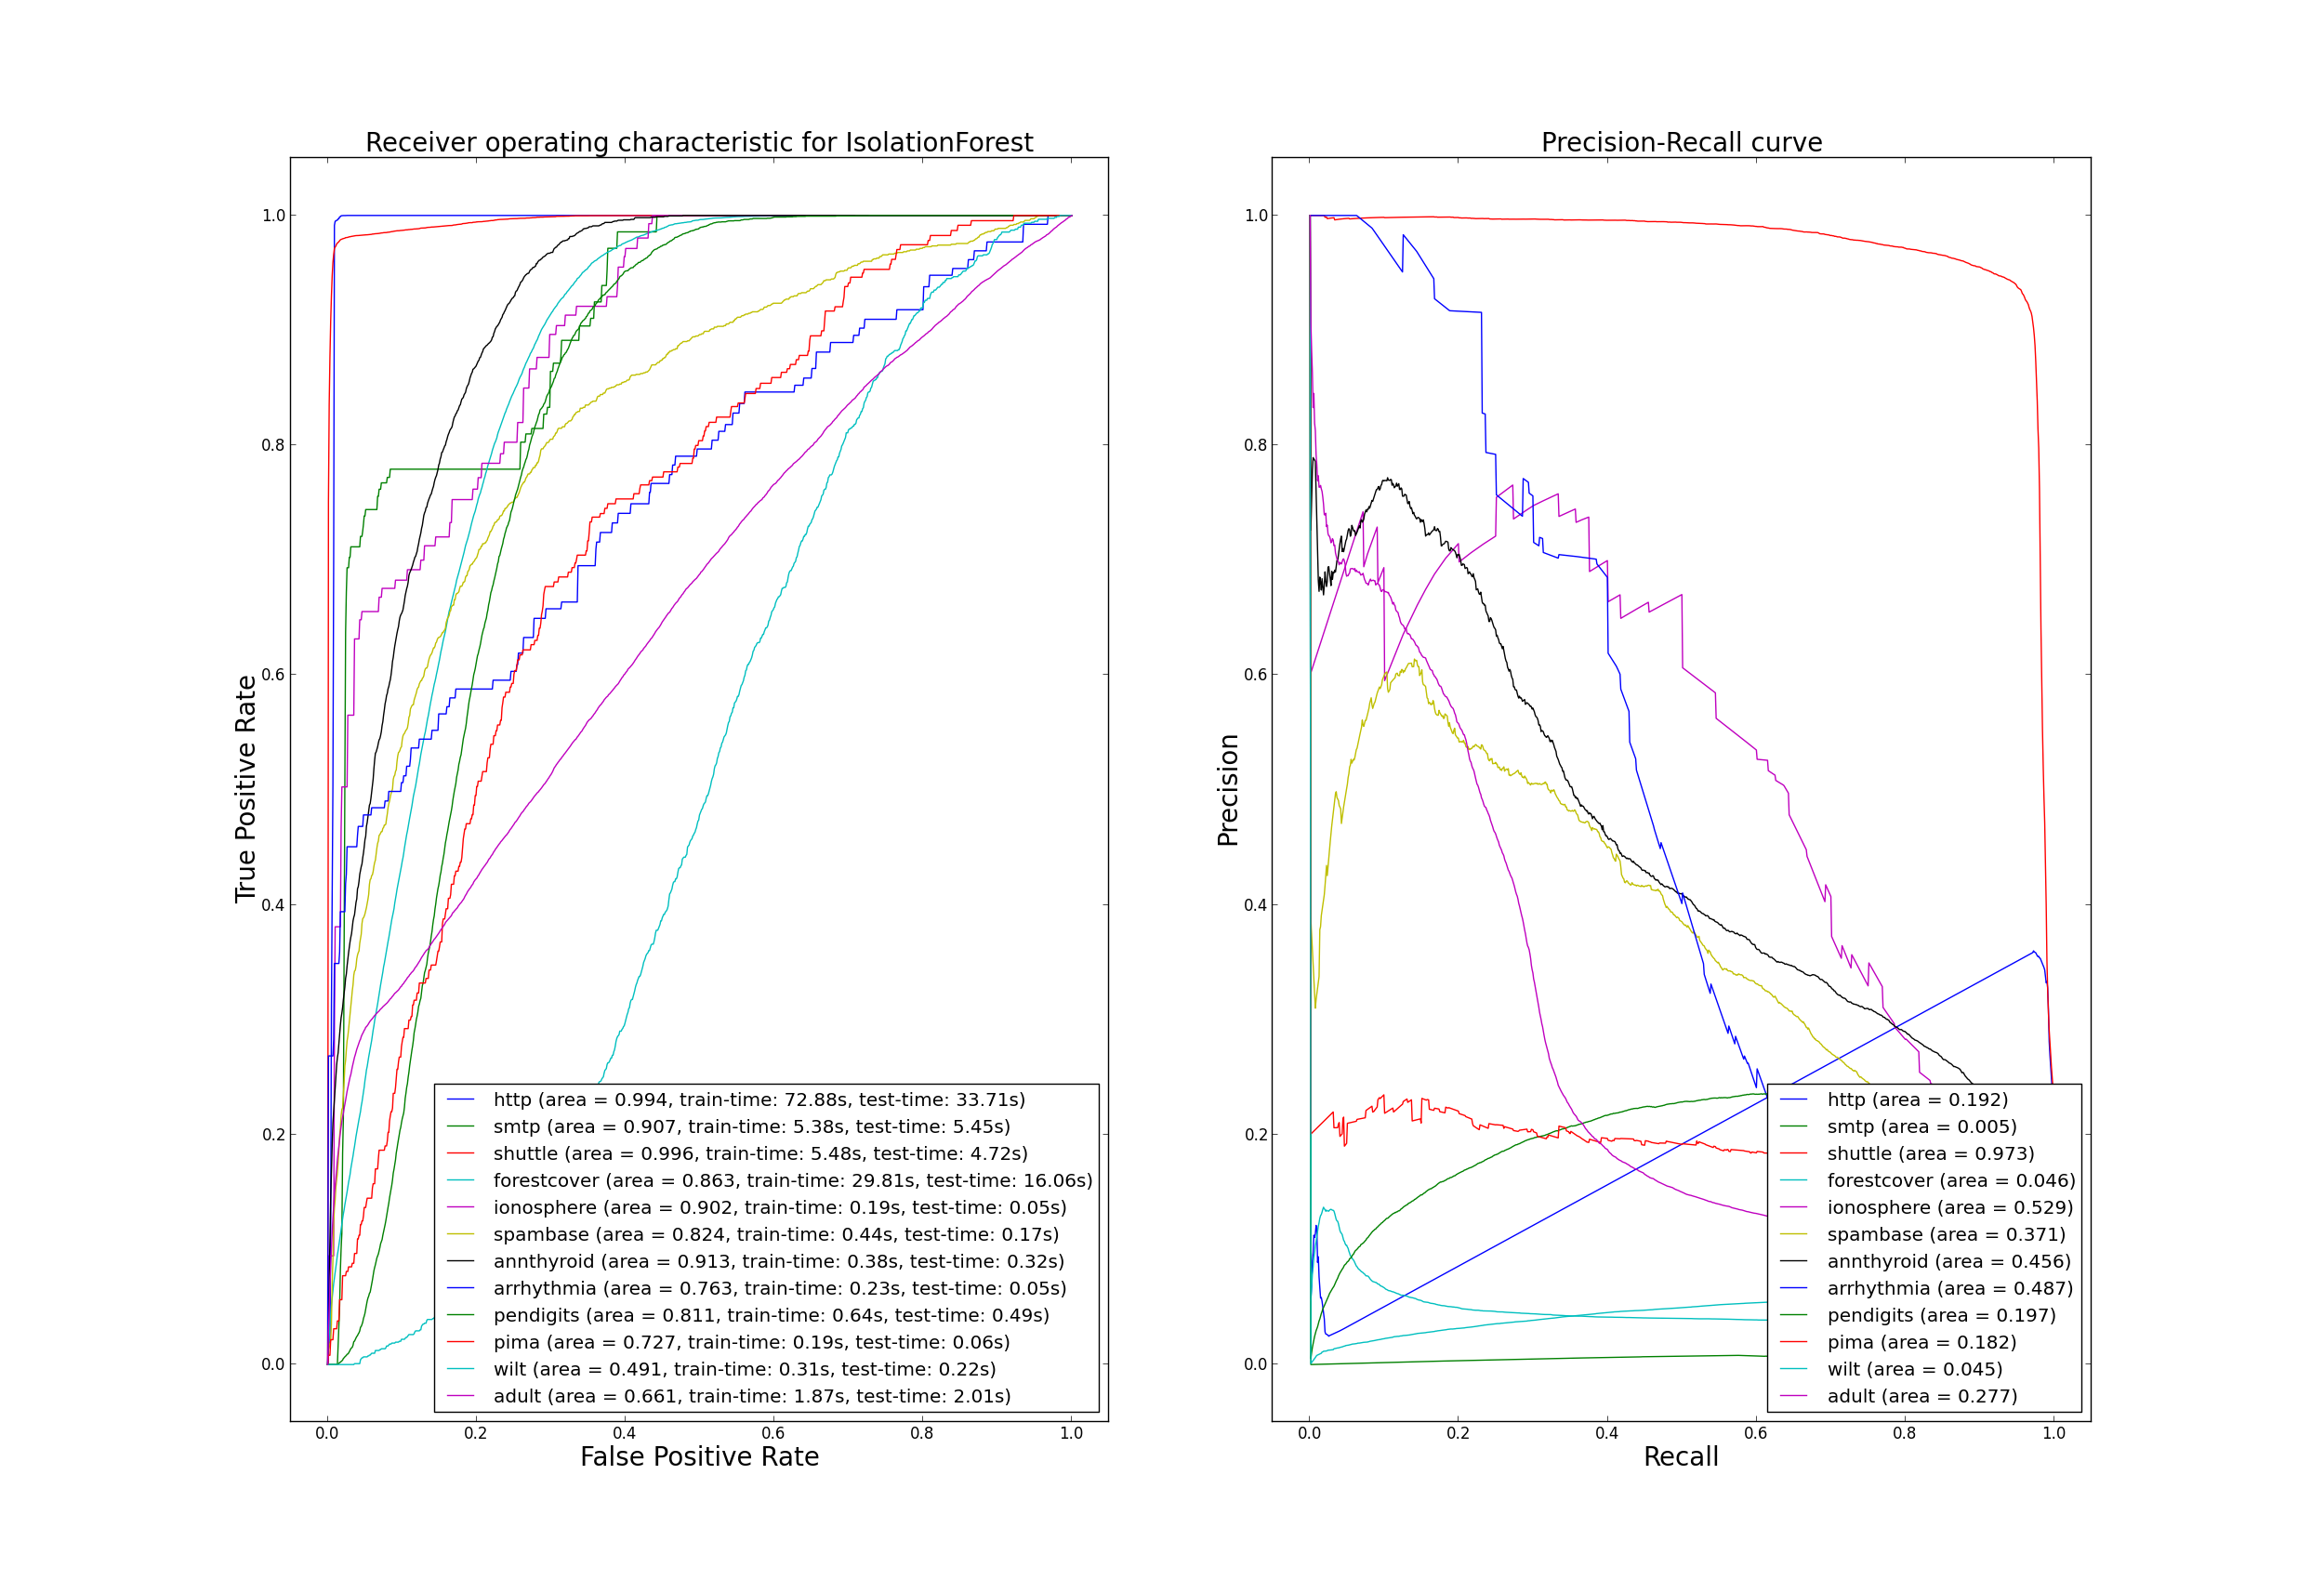
\includegraphics[trim=175 80 175 98, clip, width=0.98\linewidth]{fig_source/evaluation_fig/bench_iforest_roc_pr_supervised_factorized.png}
\end{figure}

\begin{figure}[!ht]
  \centering
  \label{evaluation:fig:iforest_roc_pr_unsupervised}
  \caption{ROC and PR curves for Isolation Forest (unsupervised framework)}
  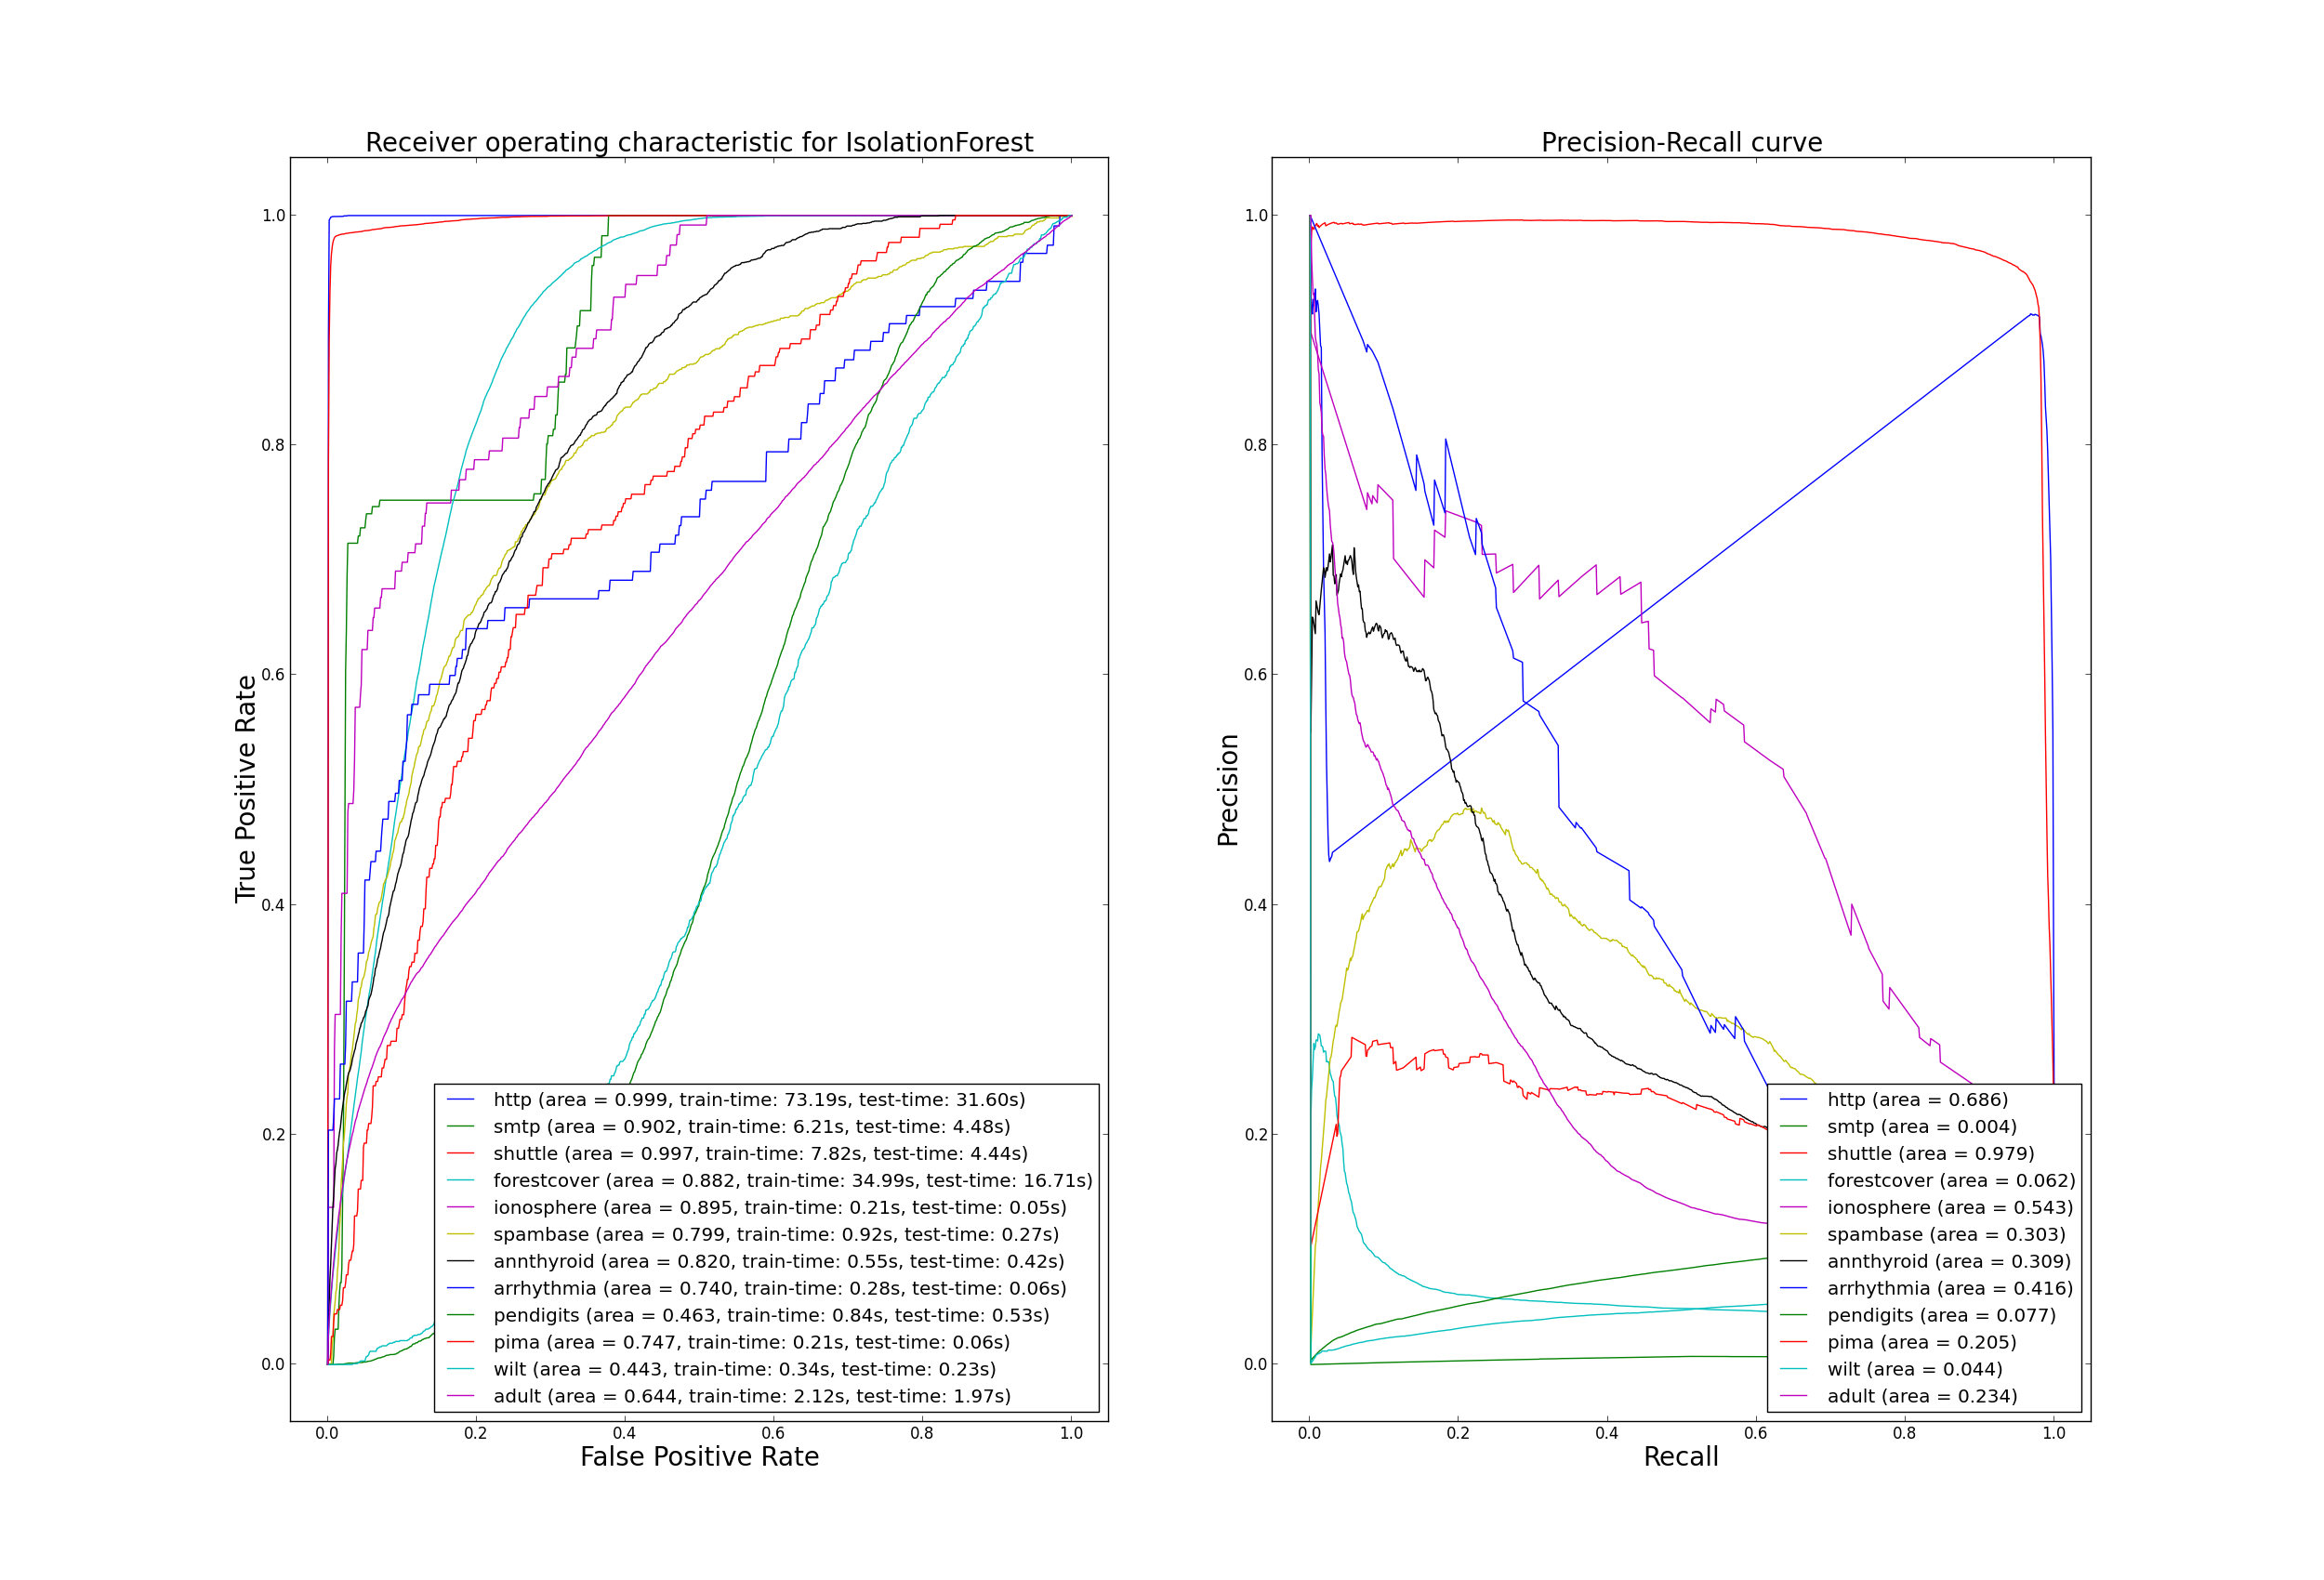
\includegraphics[trim=175 80 175 98, clip, width=0.98\linewidth]{fig_source/evaluation_fig/bench_iforest_roc_pr_unsupervised_factorized.png}
\end{figure}

\begin{figure}[!ht]
  \centering
  \caption{ROC and PR curves for One Class SVM (novelty detection framework)}
  \label{evaluation:fig:ocsvm_roc_pr}
  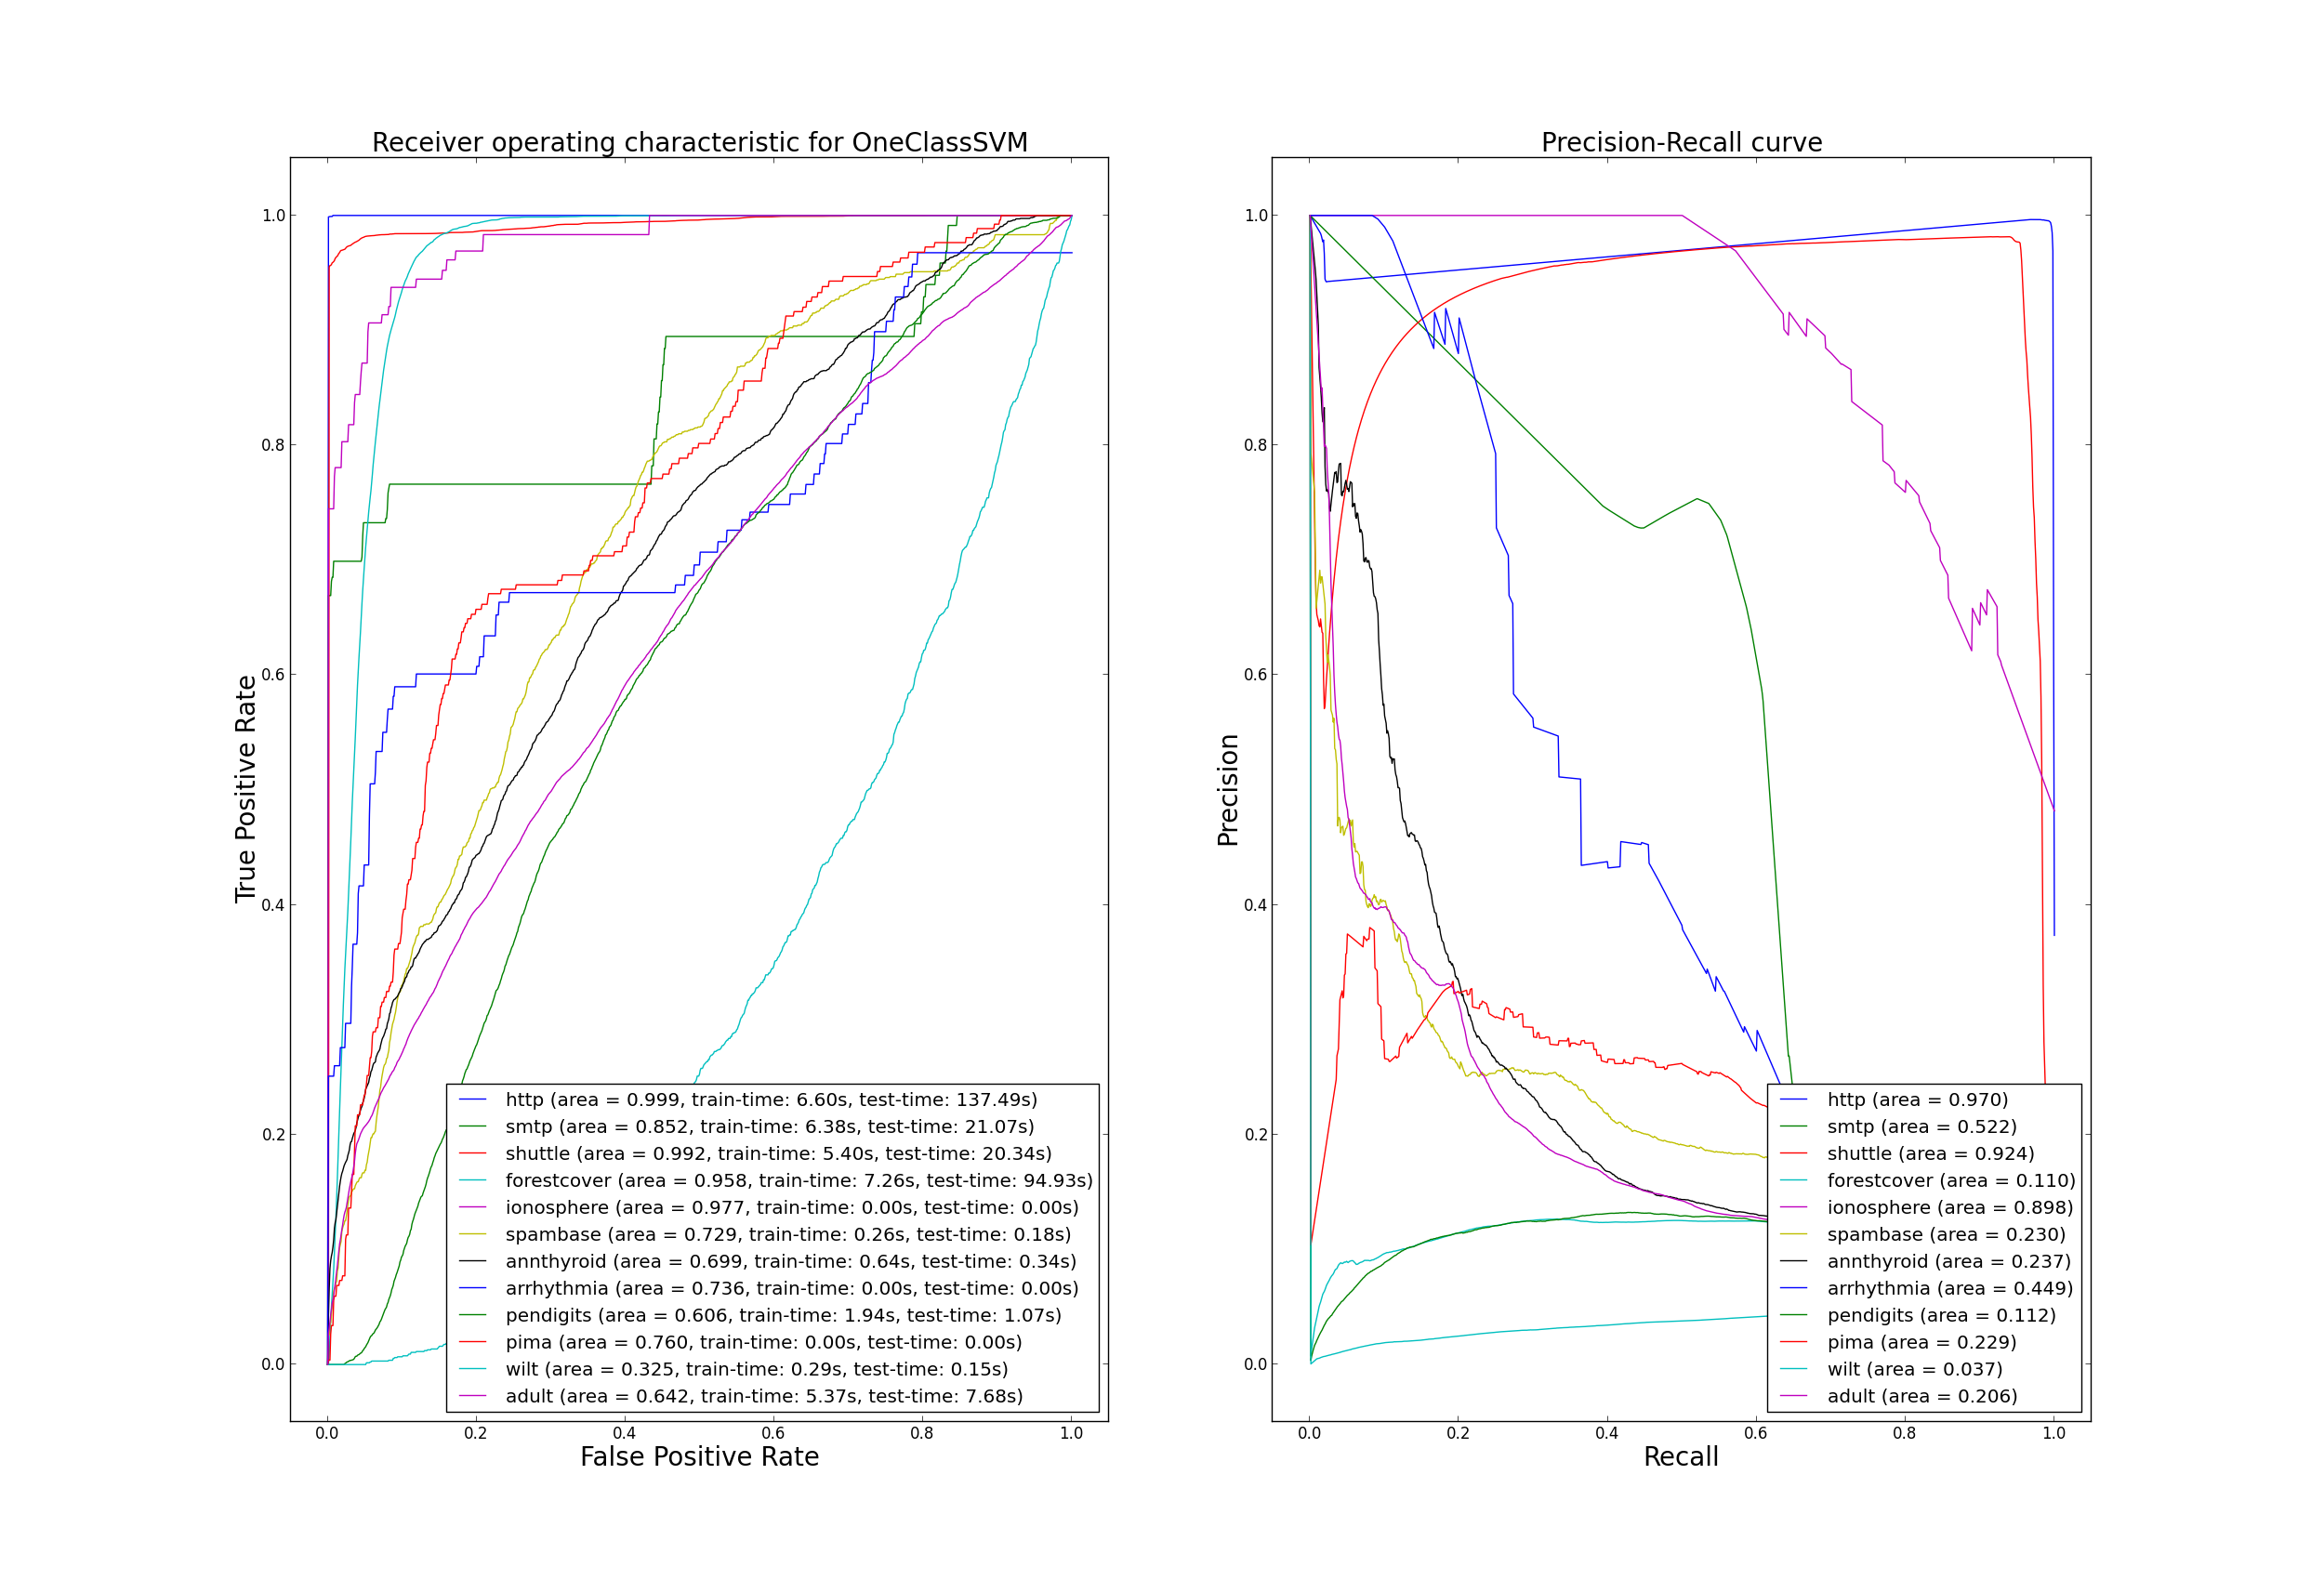
\includegraphics[trim=175 80 175 98, clip, width=\linewidth]{fig_source/evaluation_fig/bench_ocsvm_roc_pr_supervised_factorized.png}
\end{figure}

\begin{figure}[!ht]
  \centering
  \caption{ROC and PR curves for One Class SVM (unsupervised framework)}
  \label{evaluation:fig:ocsvm_roc_pr_unsupervised}
  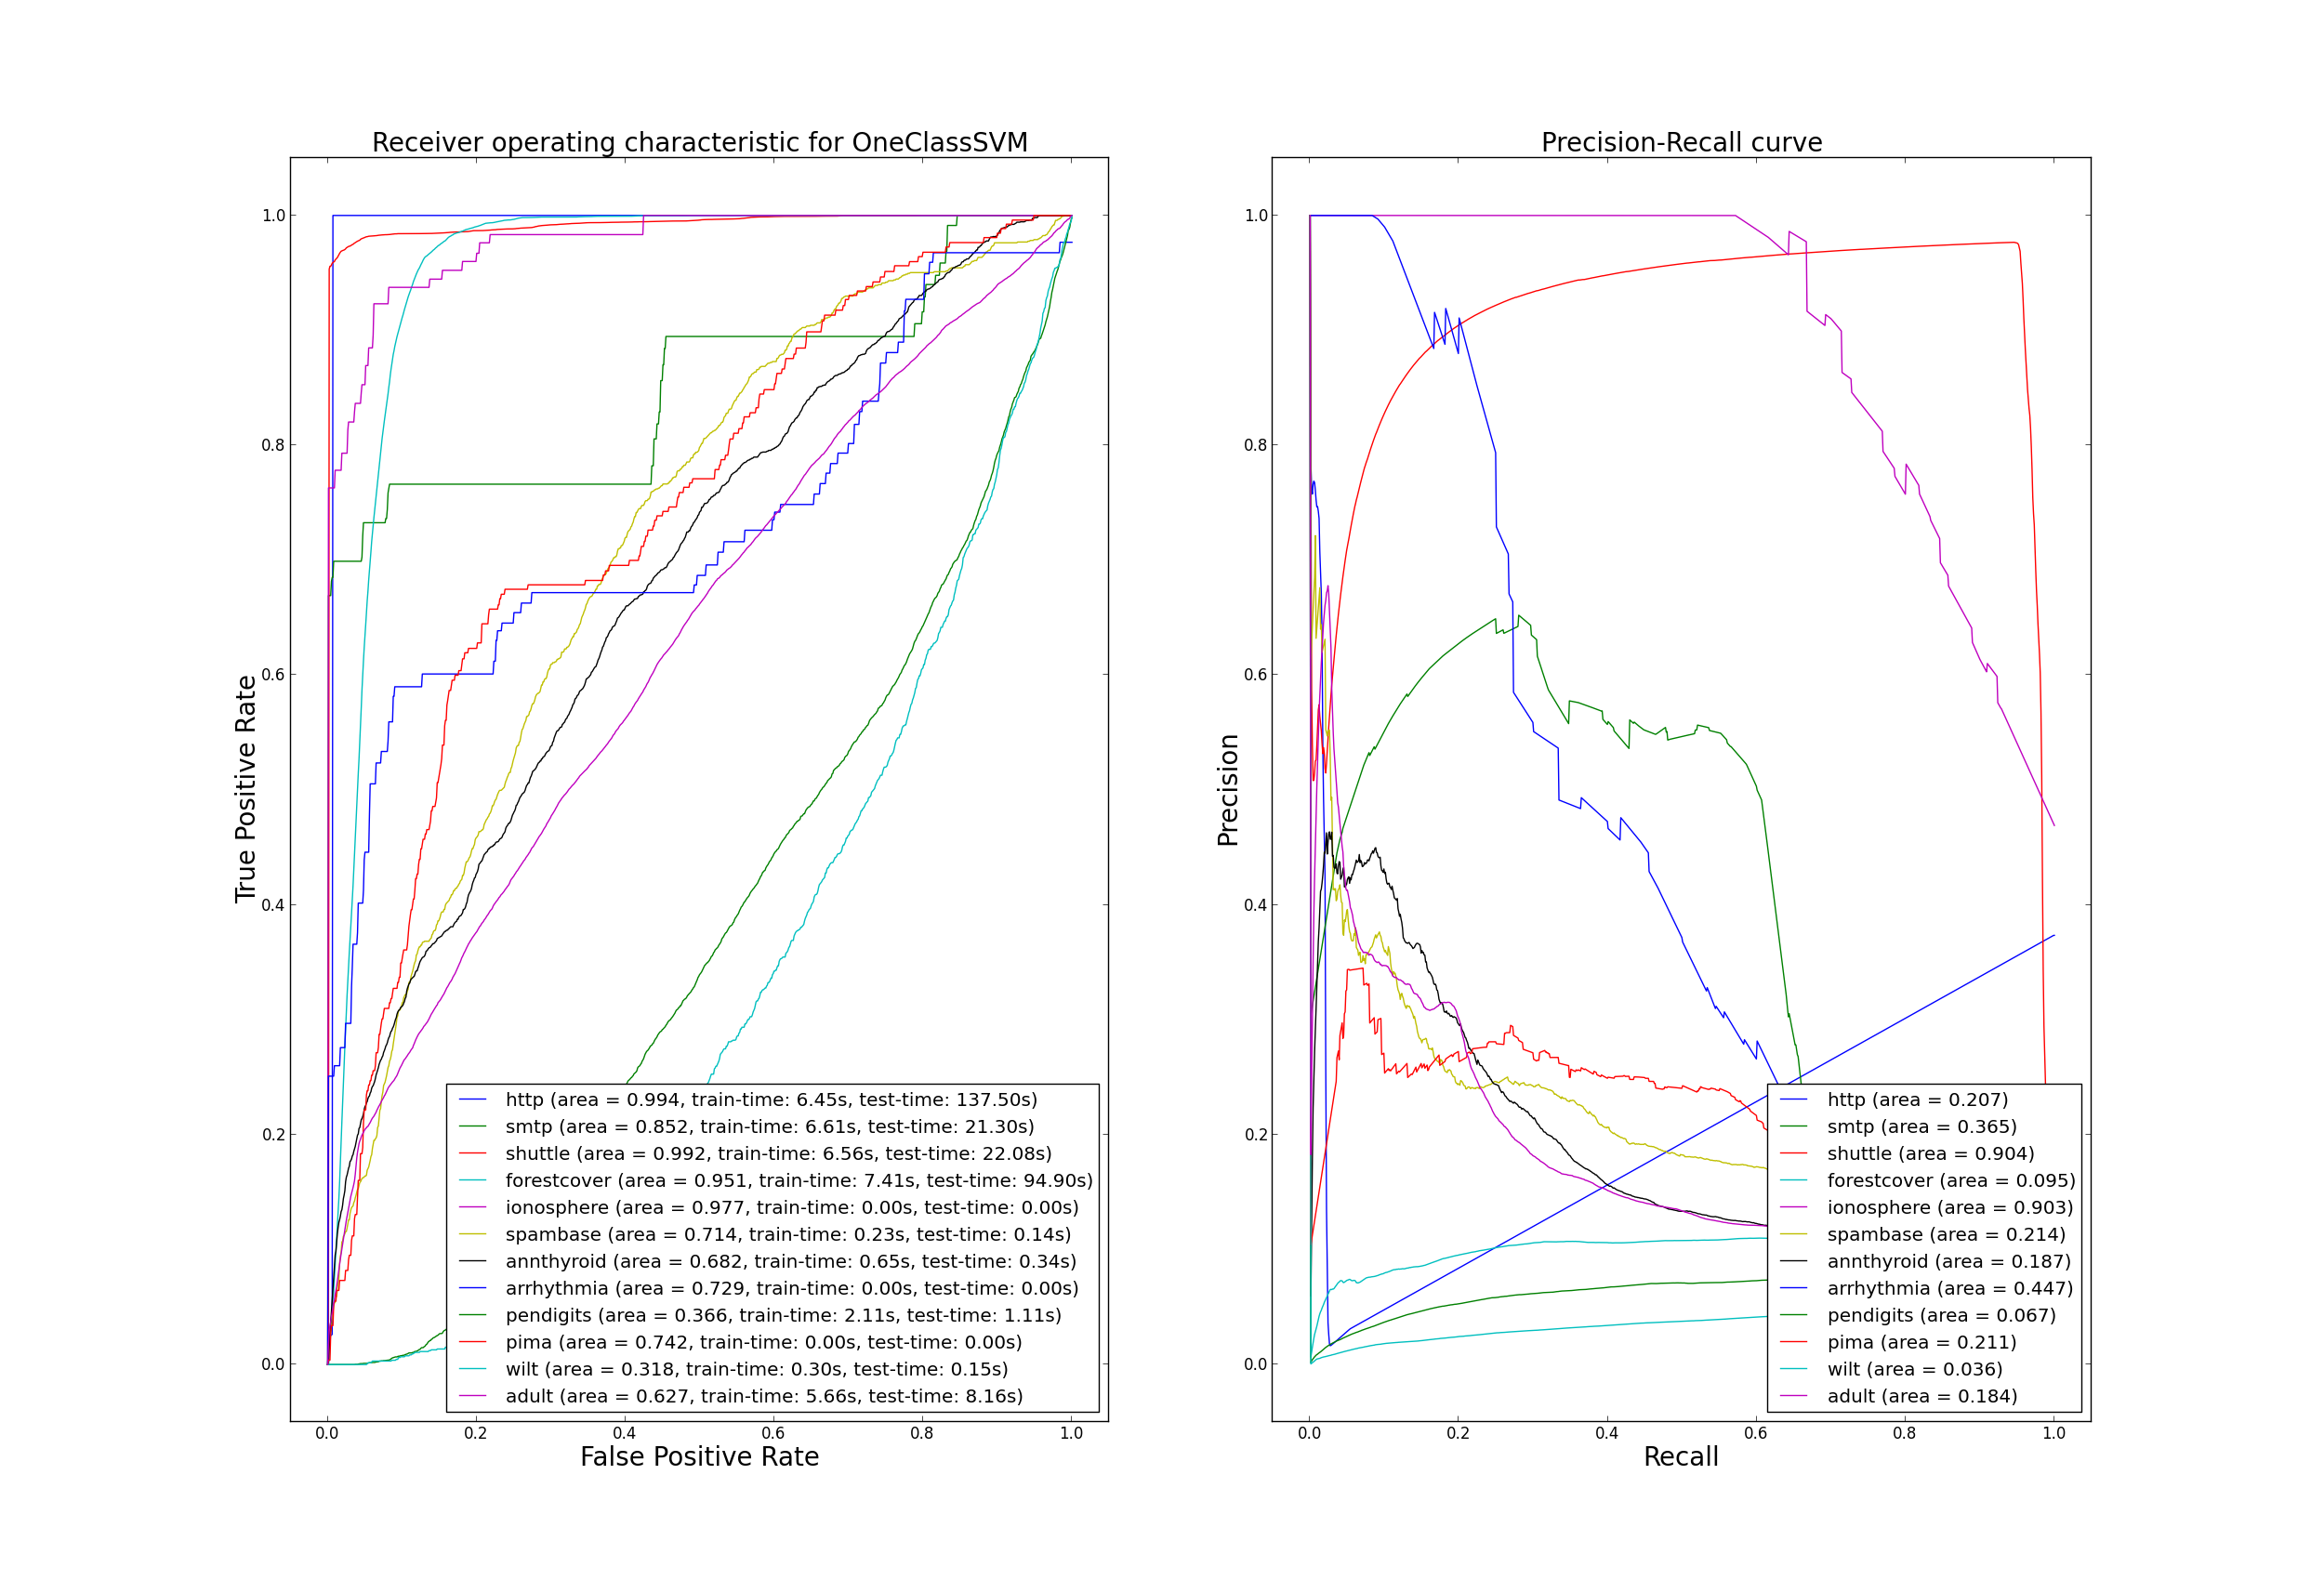
\includegraphics[trim=175 80 175 98, clip, width=\linewidth]{fig_source/evaluation_fig/bench_ocsvm_roc_pr_unsupervised_factorized.png}
\end{figure}

\begin{figure}[!ht]
  \centering
  \caption{ROC and PR curves for Local Outlier Factor (novelty detection framework)}
  \label{evaluation:fig:lof_roc_pr}
  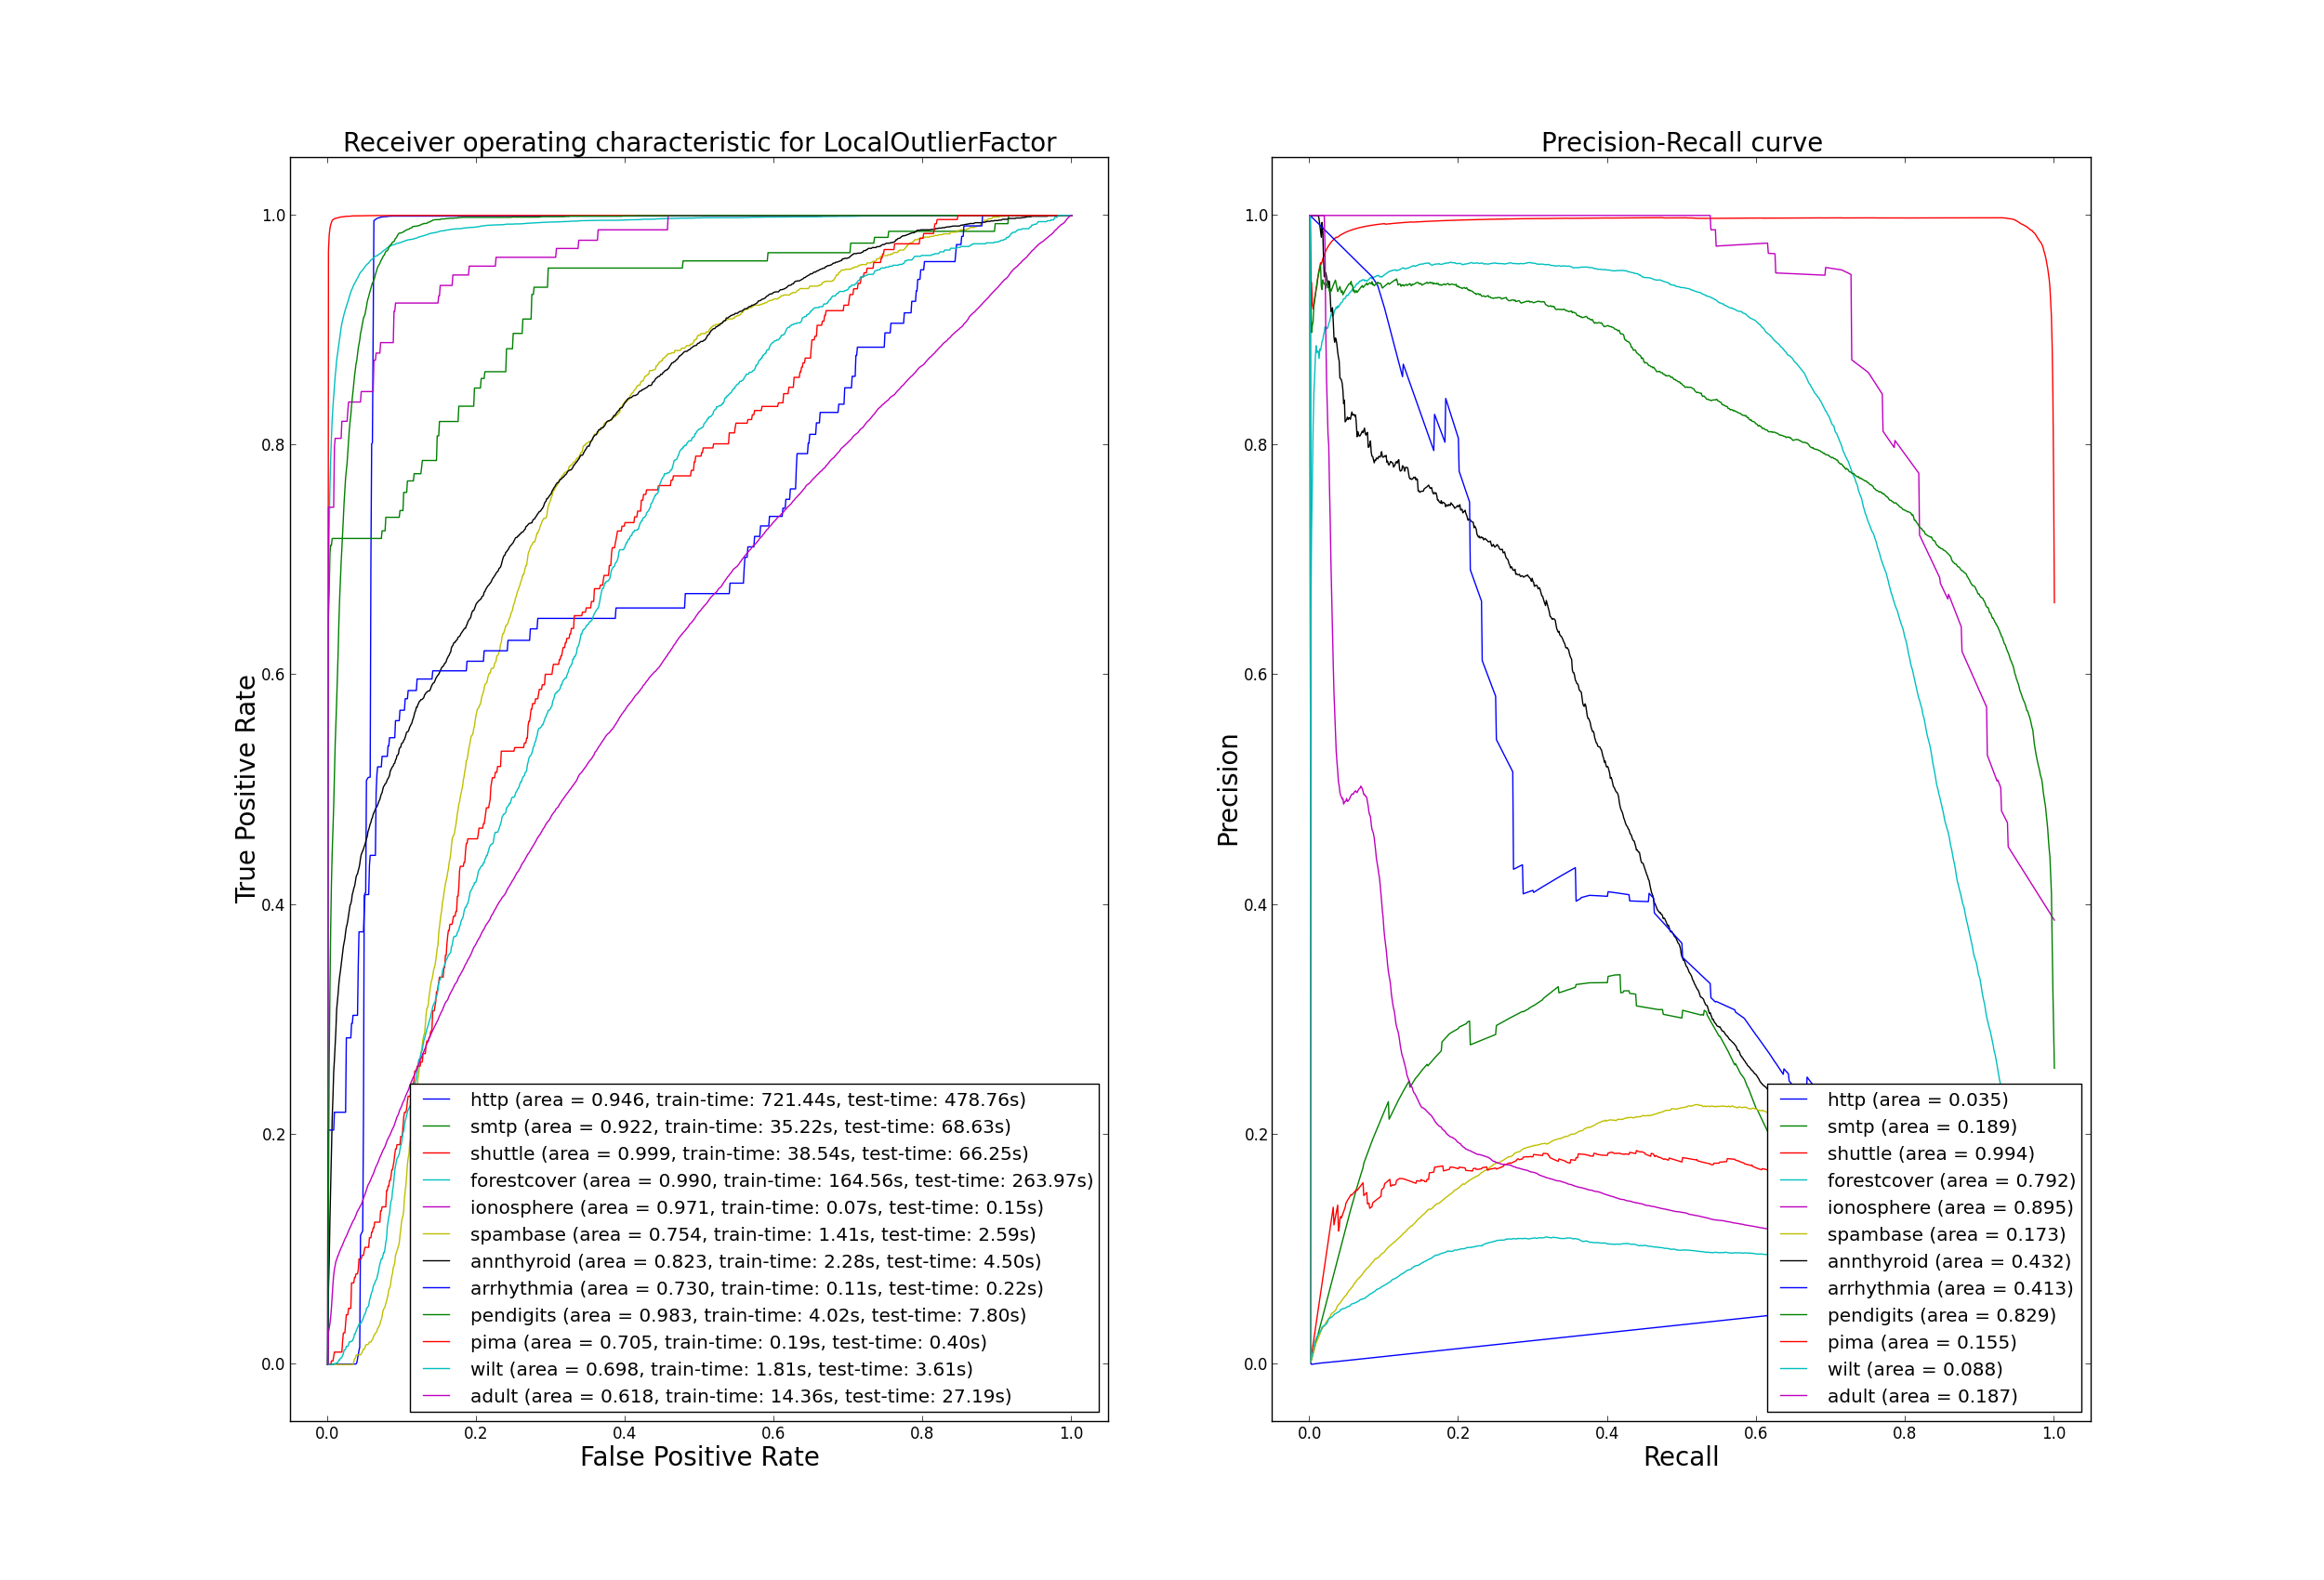
\includegraphics[trim=175 80 175 98, clip, width=\linewidth]{fig_source/evaluation_fig/bench_lof_roc_pr_supervised_factorized.png}
\end{figure}

\begin{figure}[!ht]
  \centering
  \caption{ROC and PR curves for Local Outlier Factor (unsupervised framework)}
  \label{evaluation:fig:lof_roc_pr_unsupervised}
  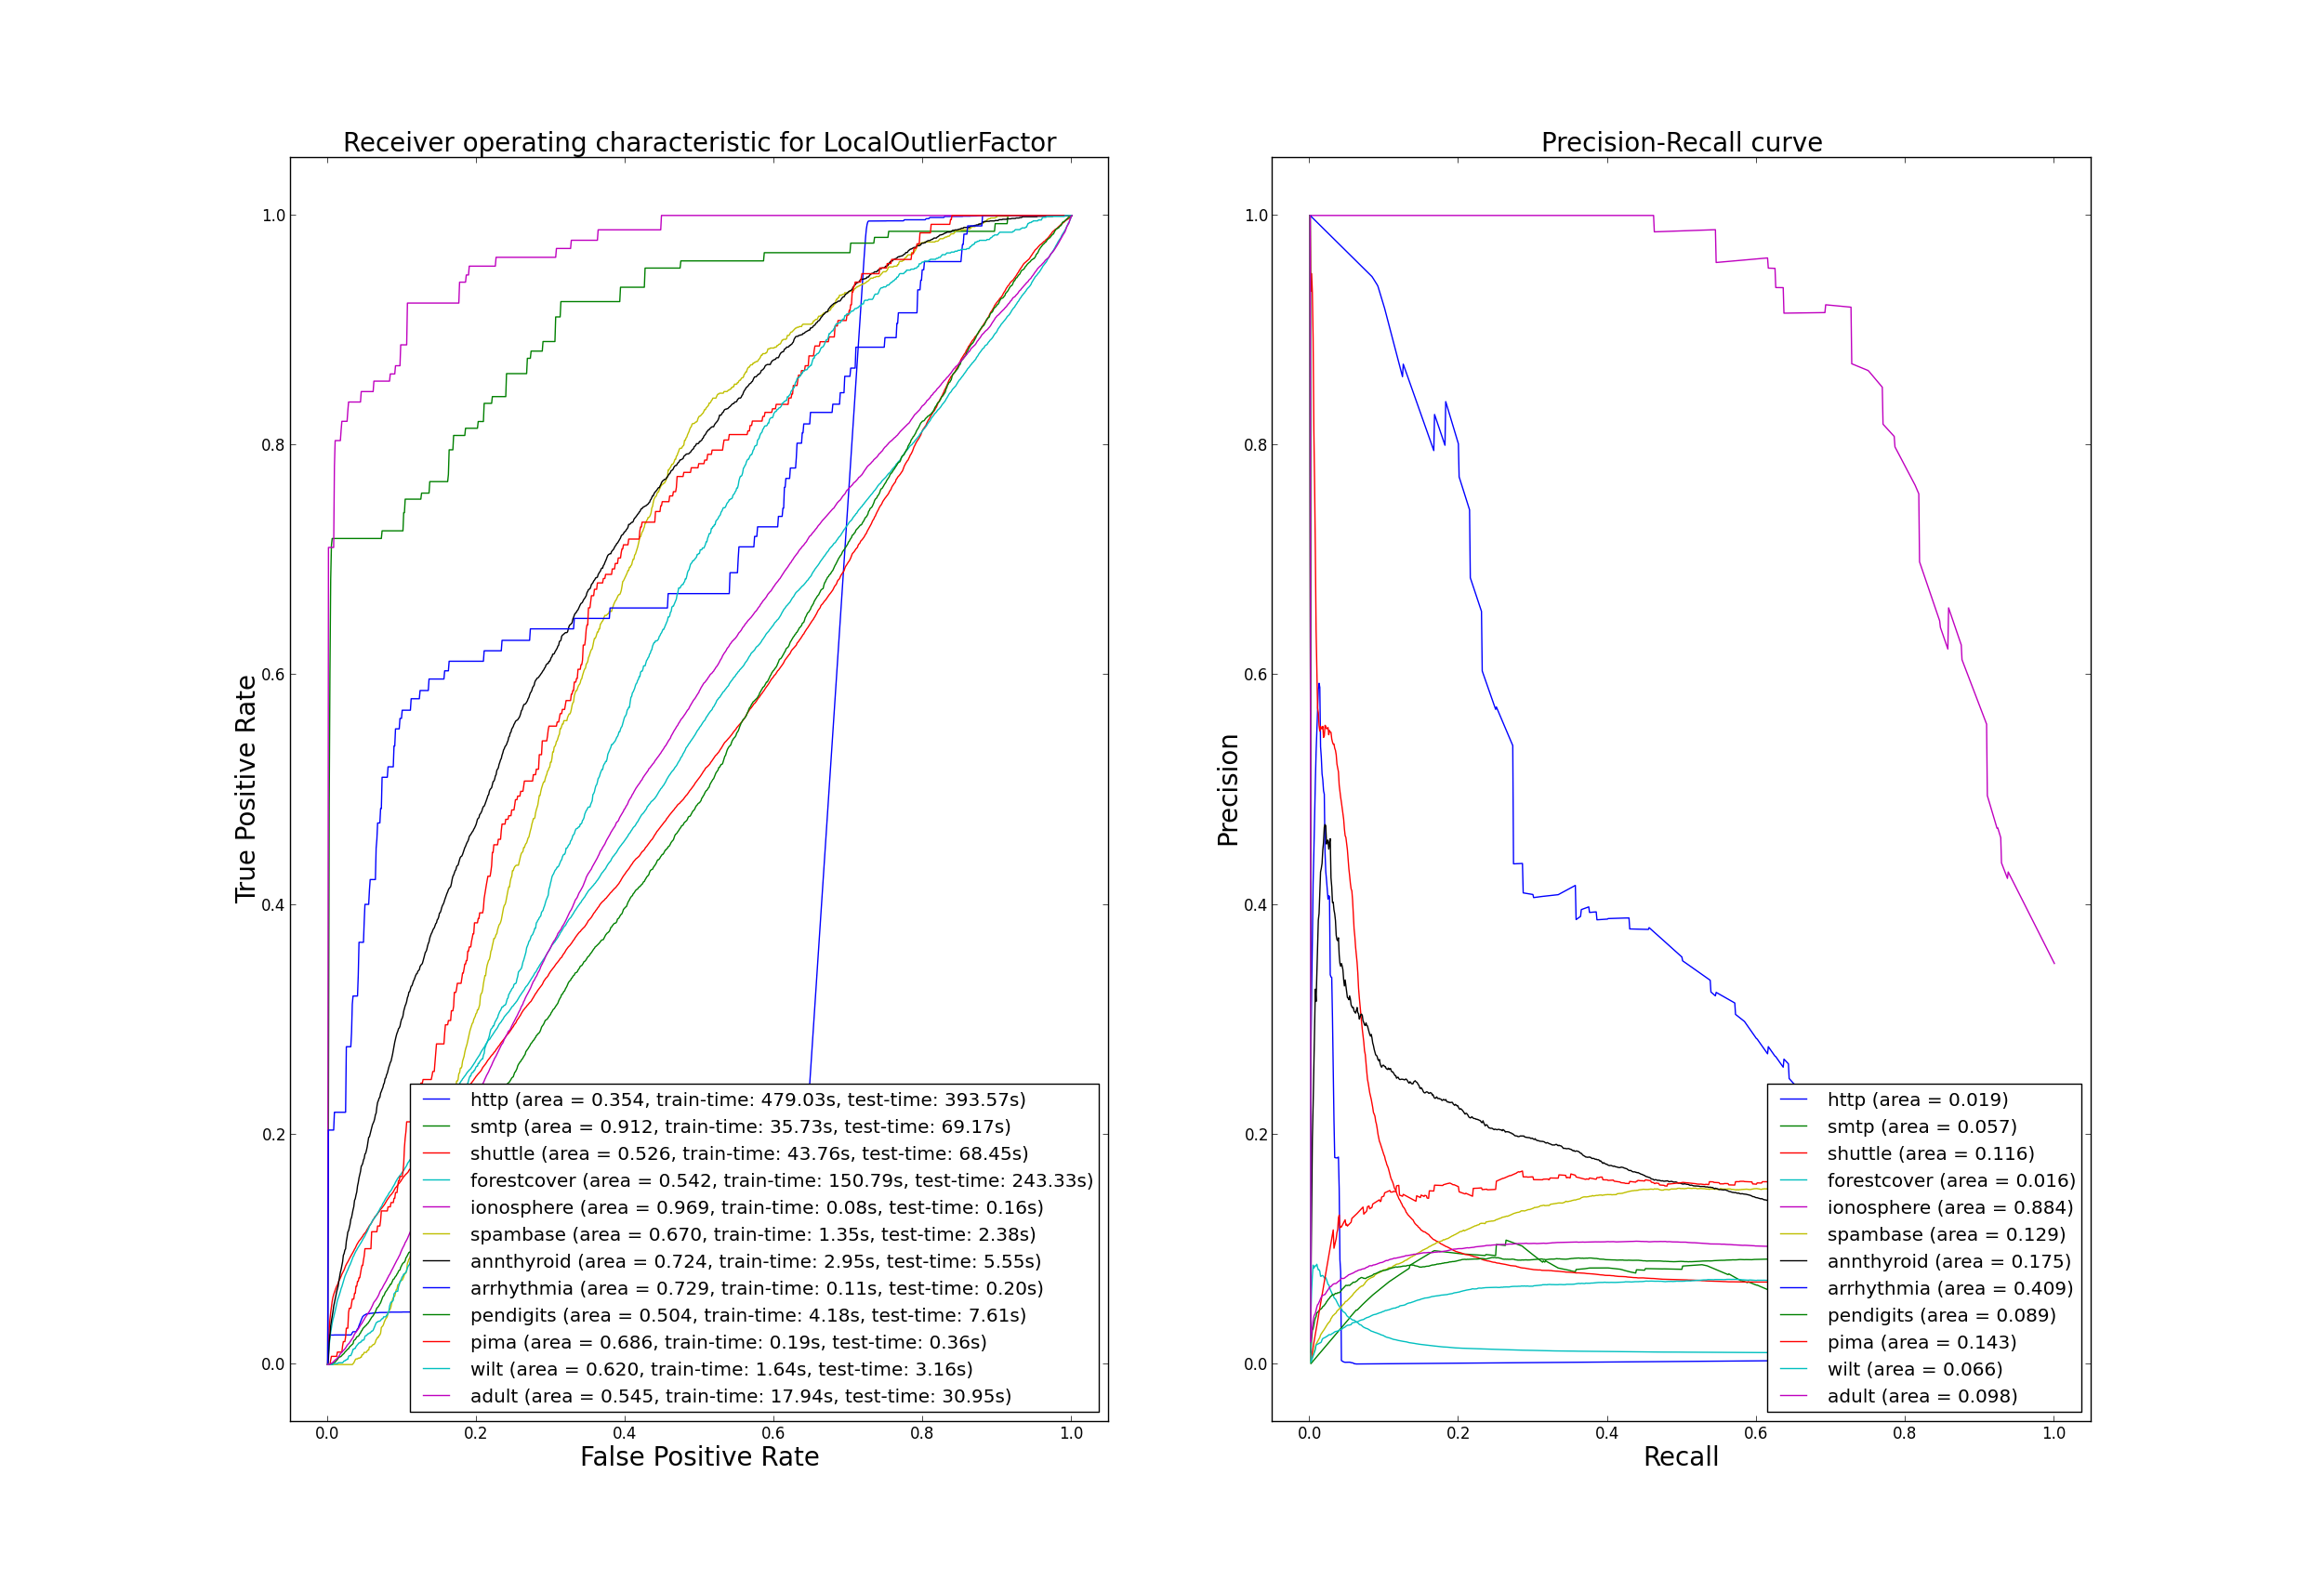
\includegraphics[trim=175 80 175 98, clip, width=\linewidth]{fig_source/evaluation_fig/bench_lof_roc_pr_unsupervised_factorized.png}
\end{figure}

%------------------------- mv_em:
%\subsection{Other EM and MV curves}
% trim=left bottom right top, clip
\begin{figure}[!ht]
\label{evaluation:mv_em_http}
  \centering
  \caption{MV and EM curves for http dataset (novelty detection framework)}
  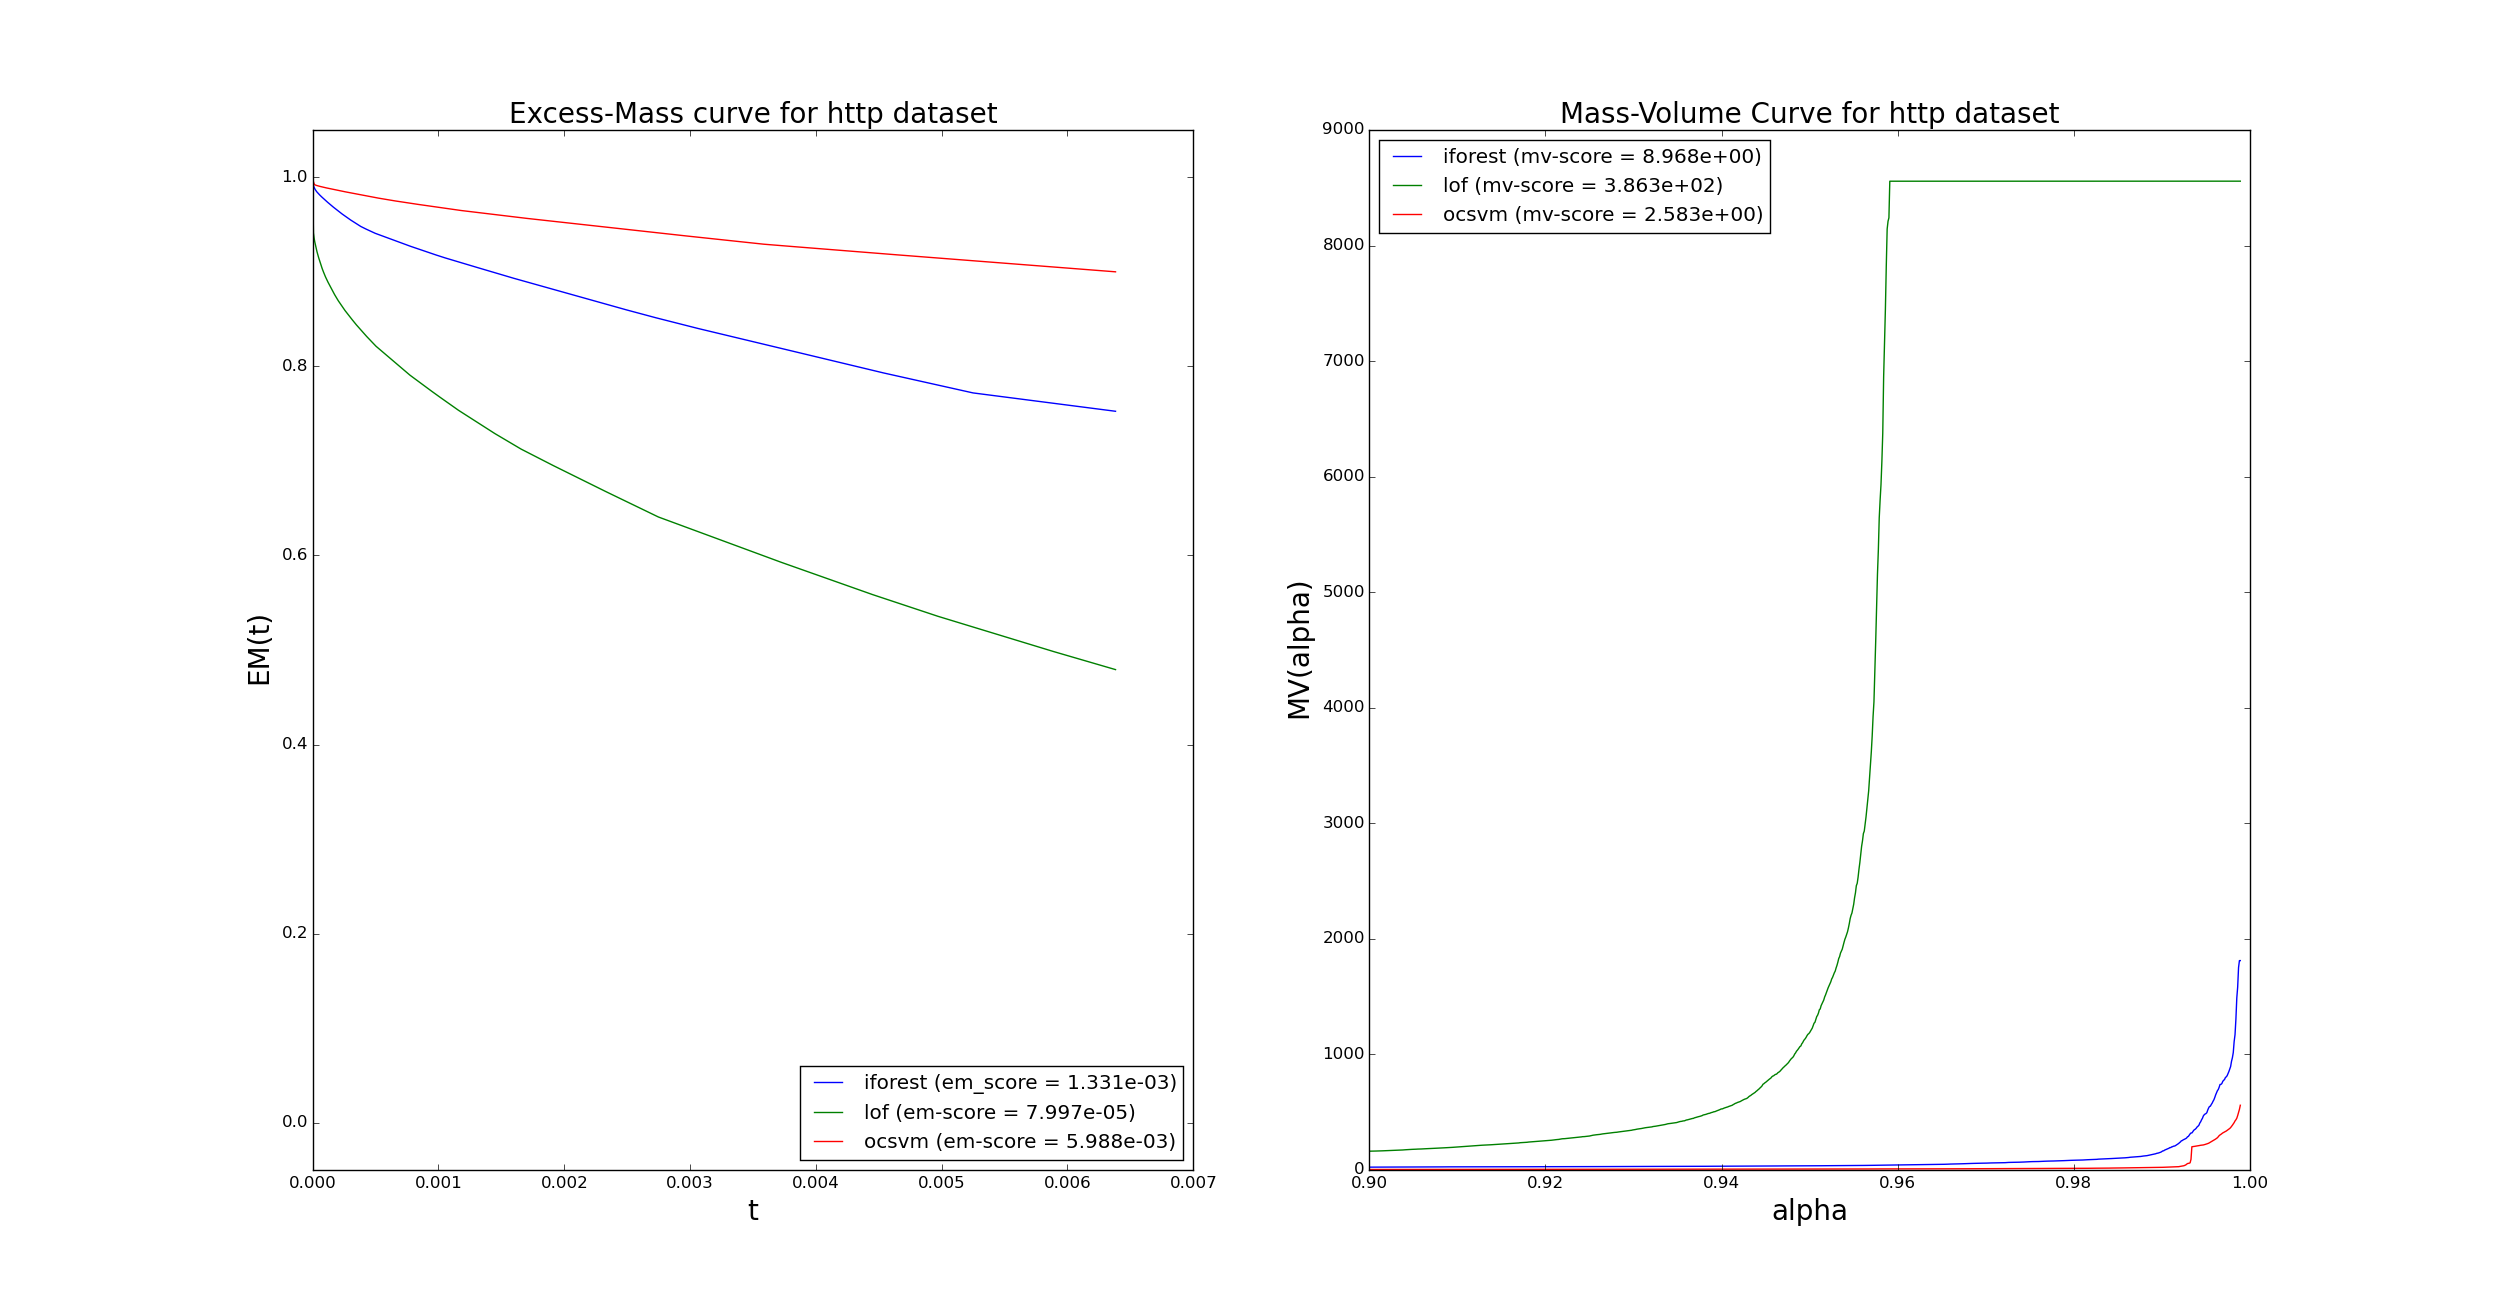
\includegraphics[trim=172 52 165 70, clip, width=\linewidth]{fig_source/evaluation_fig/mv_em_http_supervised_09_factorized.png}
\end{figure}
\begin{figure}[!ht]
\label{evaluation:mv_em_http_unsupervised}
  \centering
  \caption{MV and EM curves for http dataset (unsupervised framework)}
  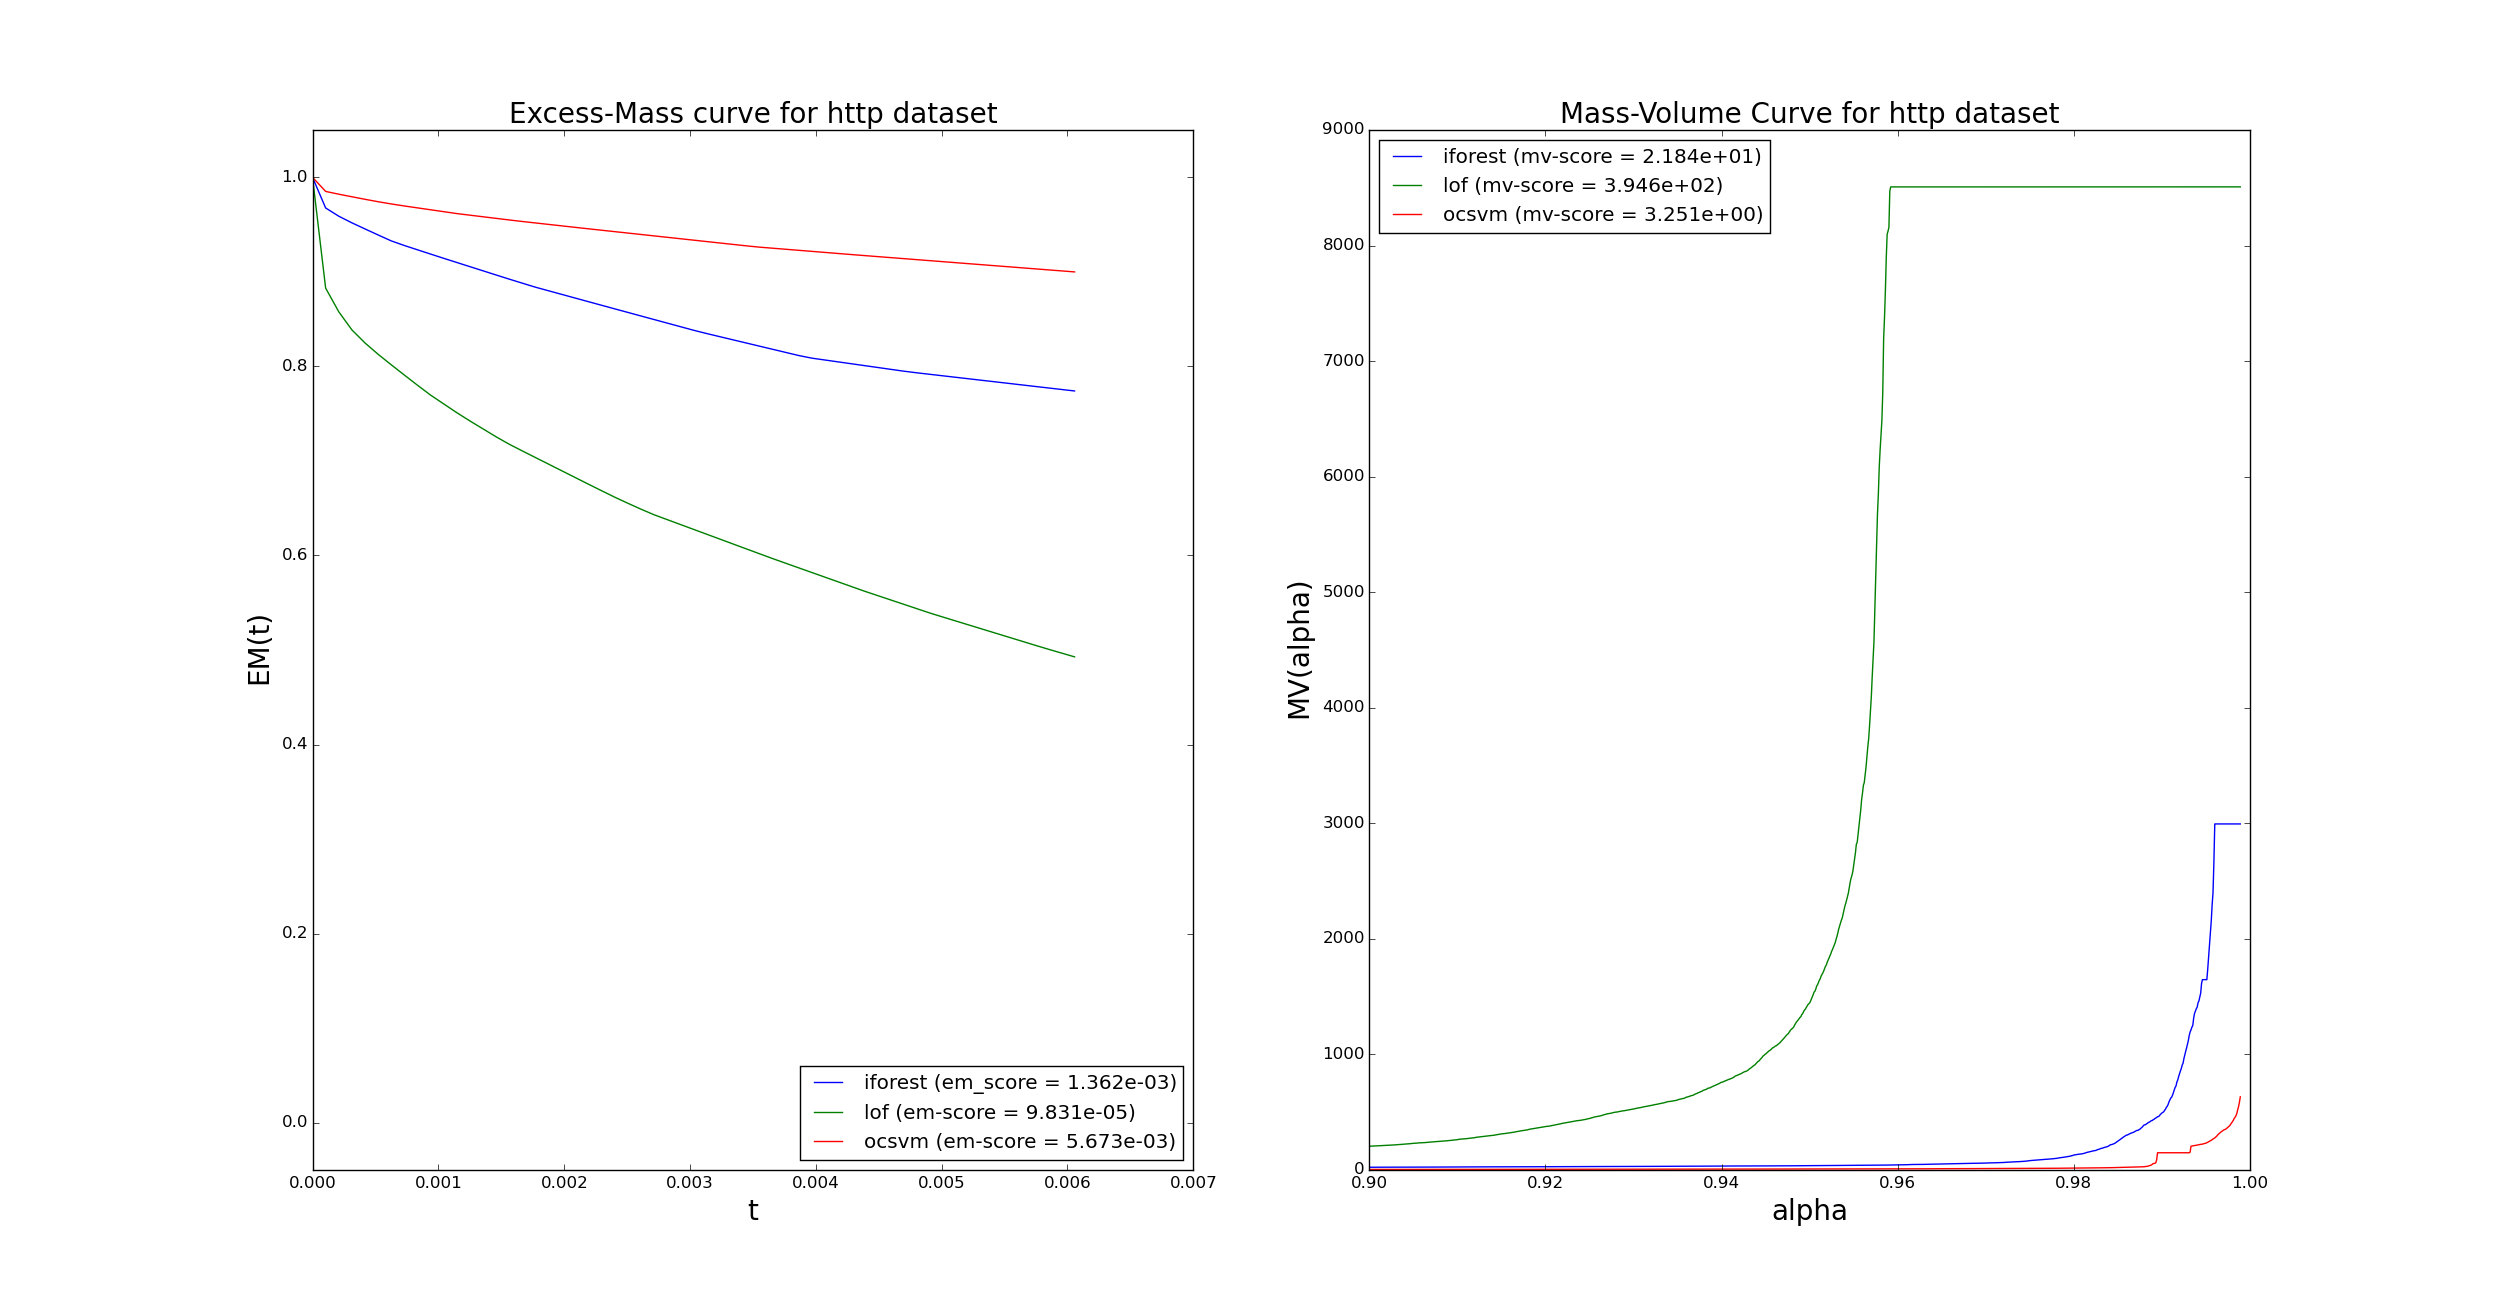
\includegraphics[trim=172 52 165 70, clip, width=\linewidth]{fig_source/evaluation_fig/mv_em_http_unsupervised_09_factorized.png}
\end{figure}

% \begin{figure}[!ht]
% \label{evaluation:mv_em_pendigits}
%   \centering
%   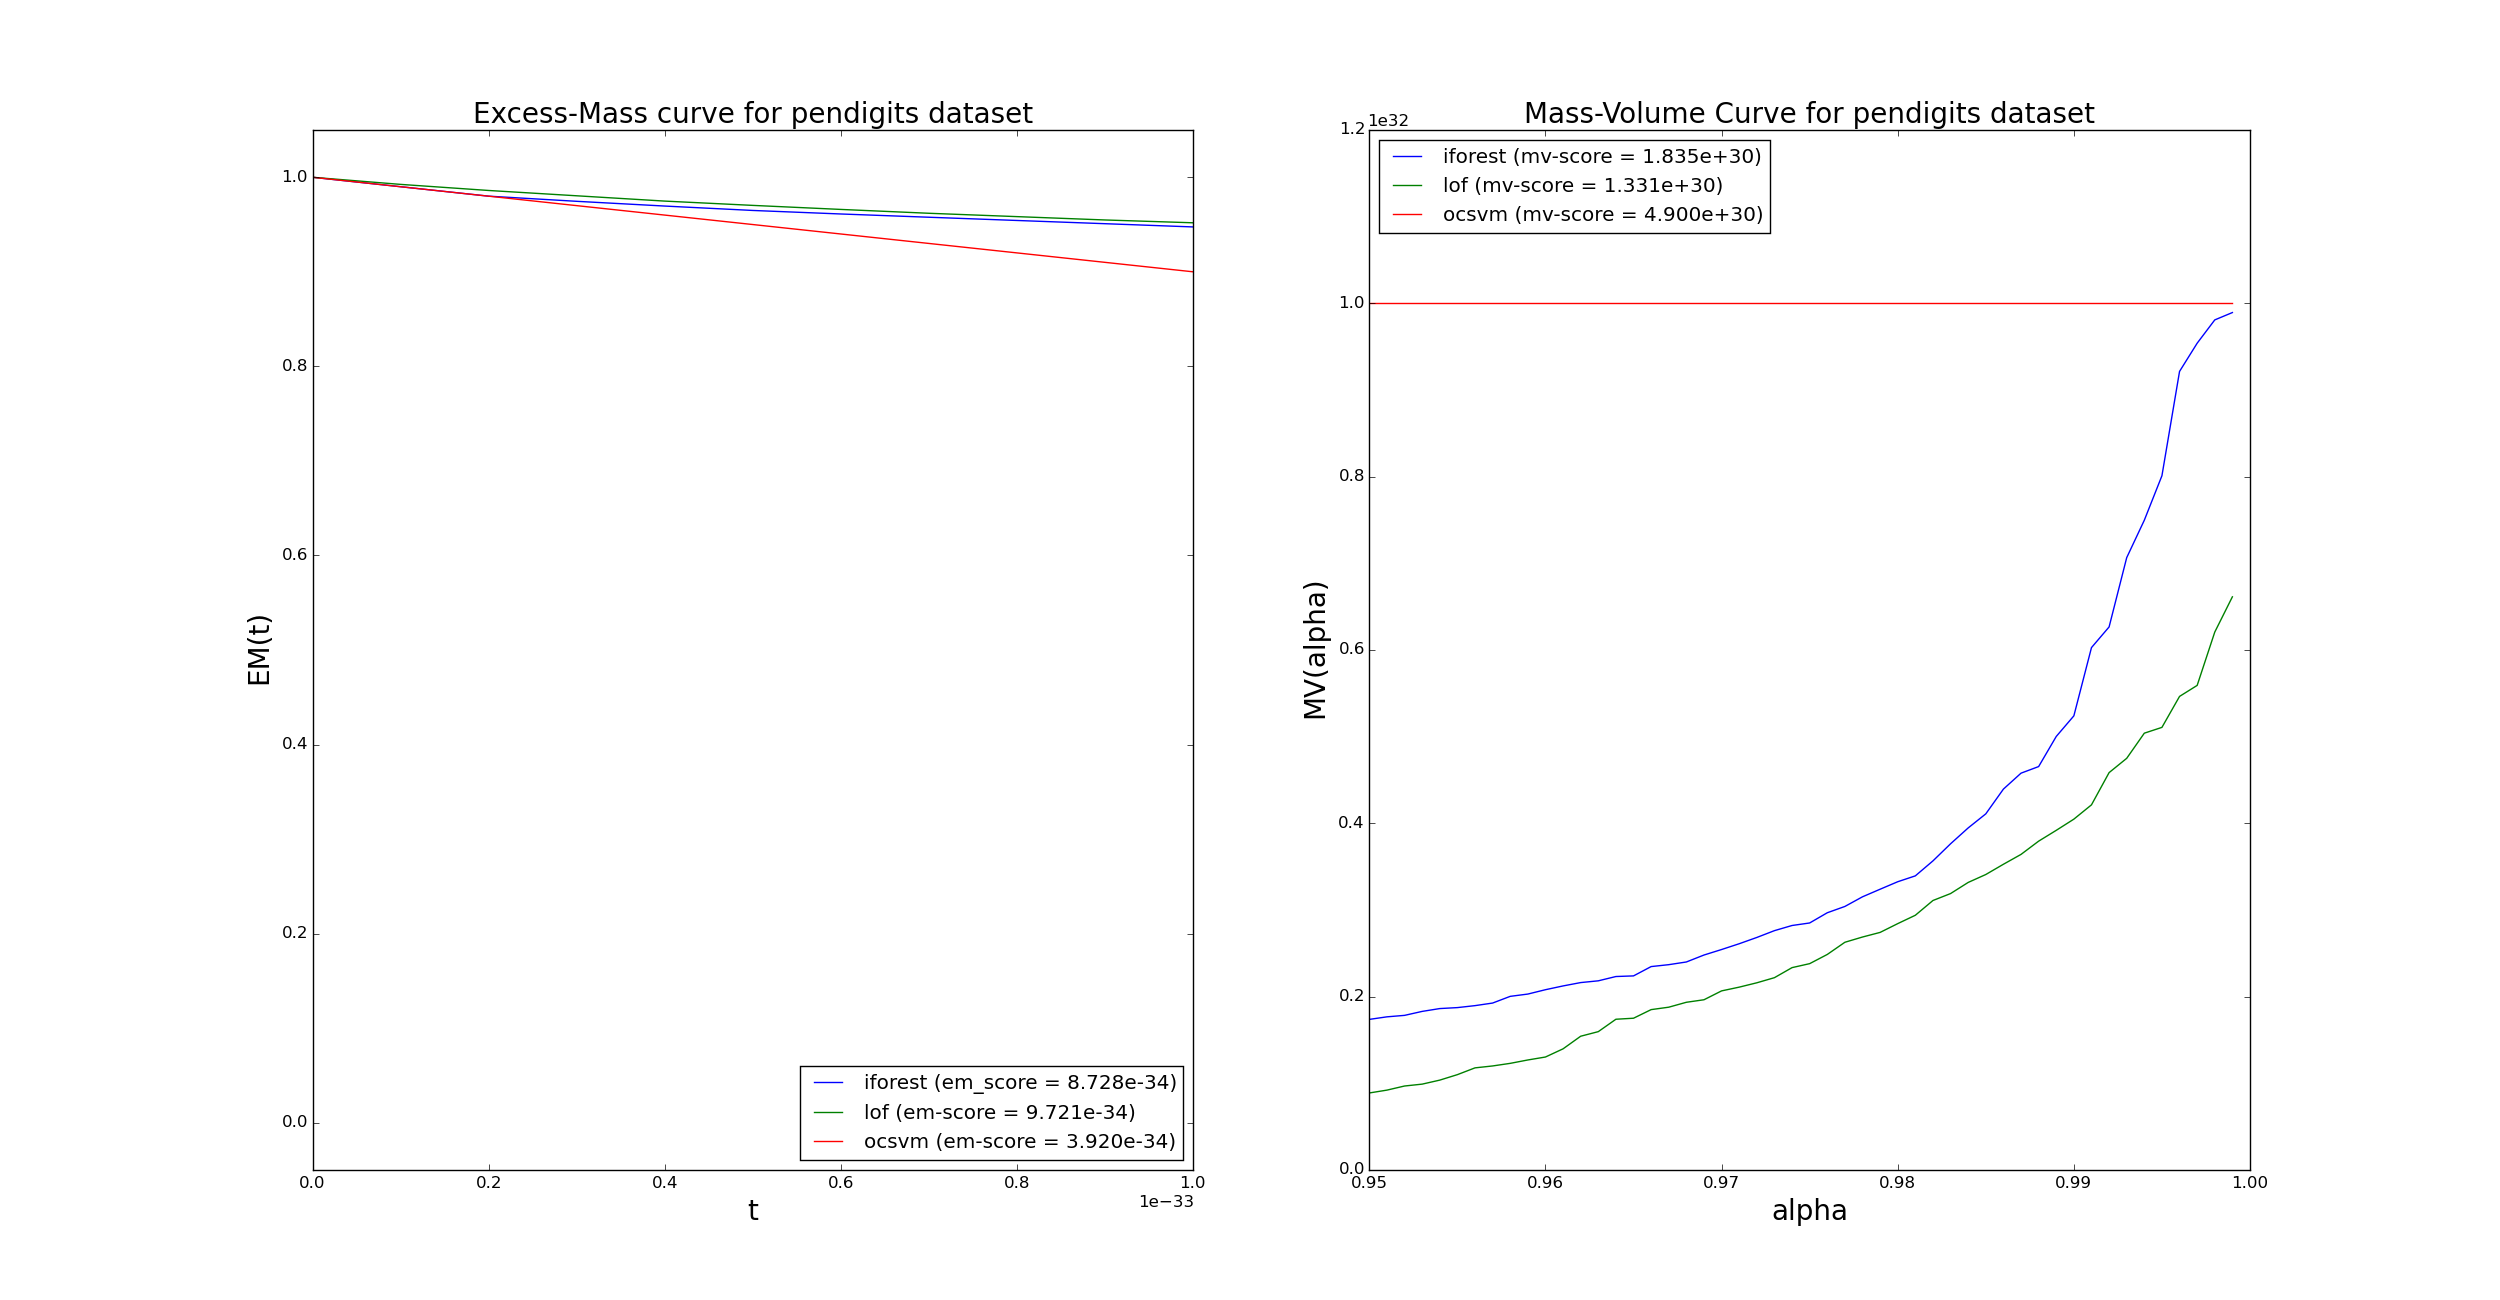
\includegraphics[trim=172 52 165 70, clip, width=\linewidth]{fig_source/evaluation_fig/t_mv_em_pendigits_supervised.png}
%   \caption{MV and EM curves for pendigits dataset (novelty detection framework)}
% \end{figure}
% \begin{figure}[!ht]
% \label{evaluation:mv_em_pendigits_unsupervised}
%   \centering
%   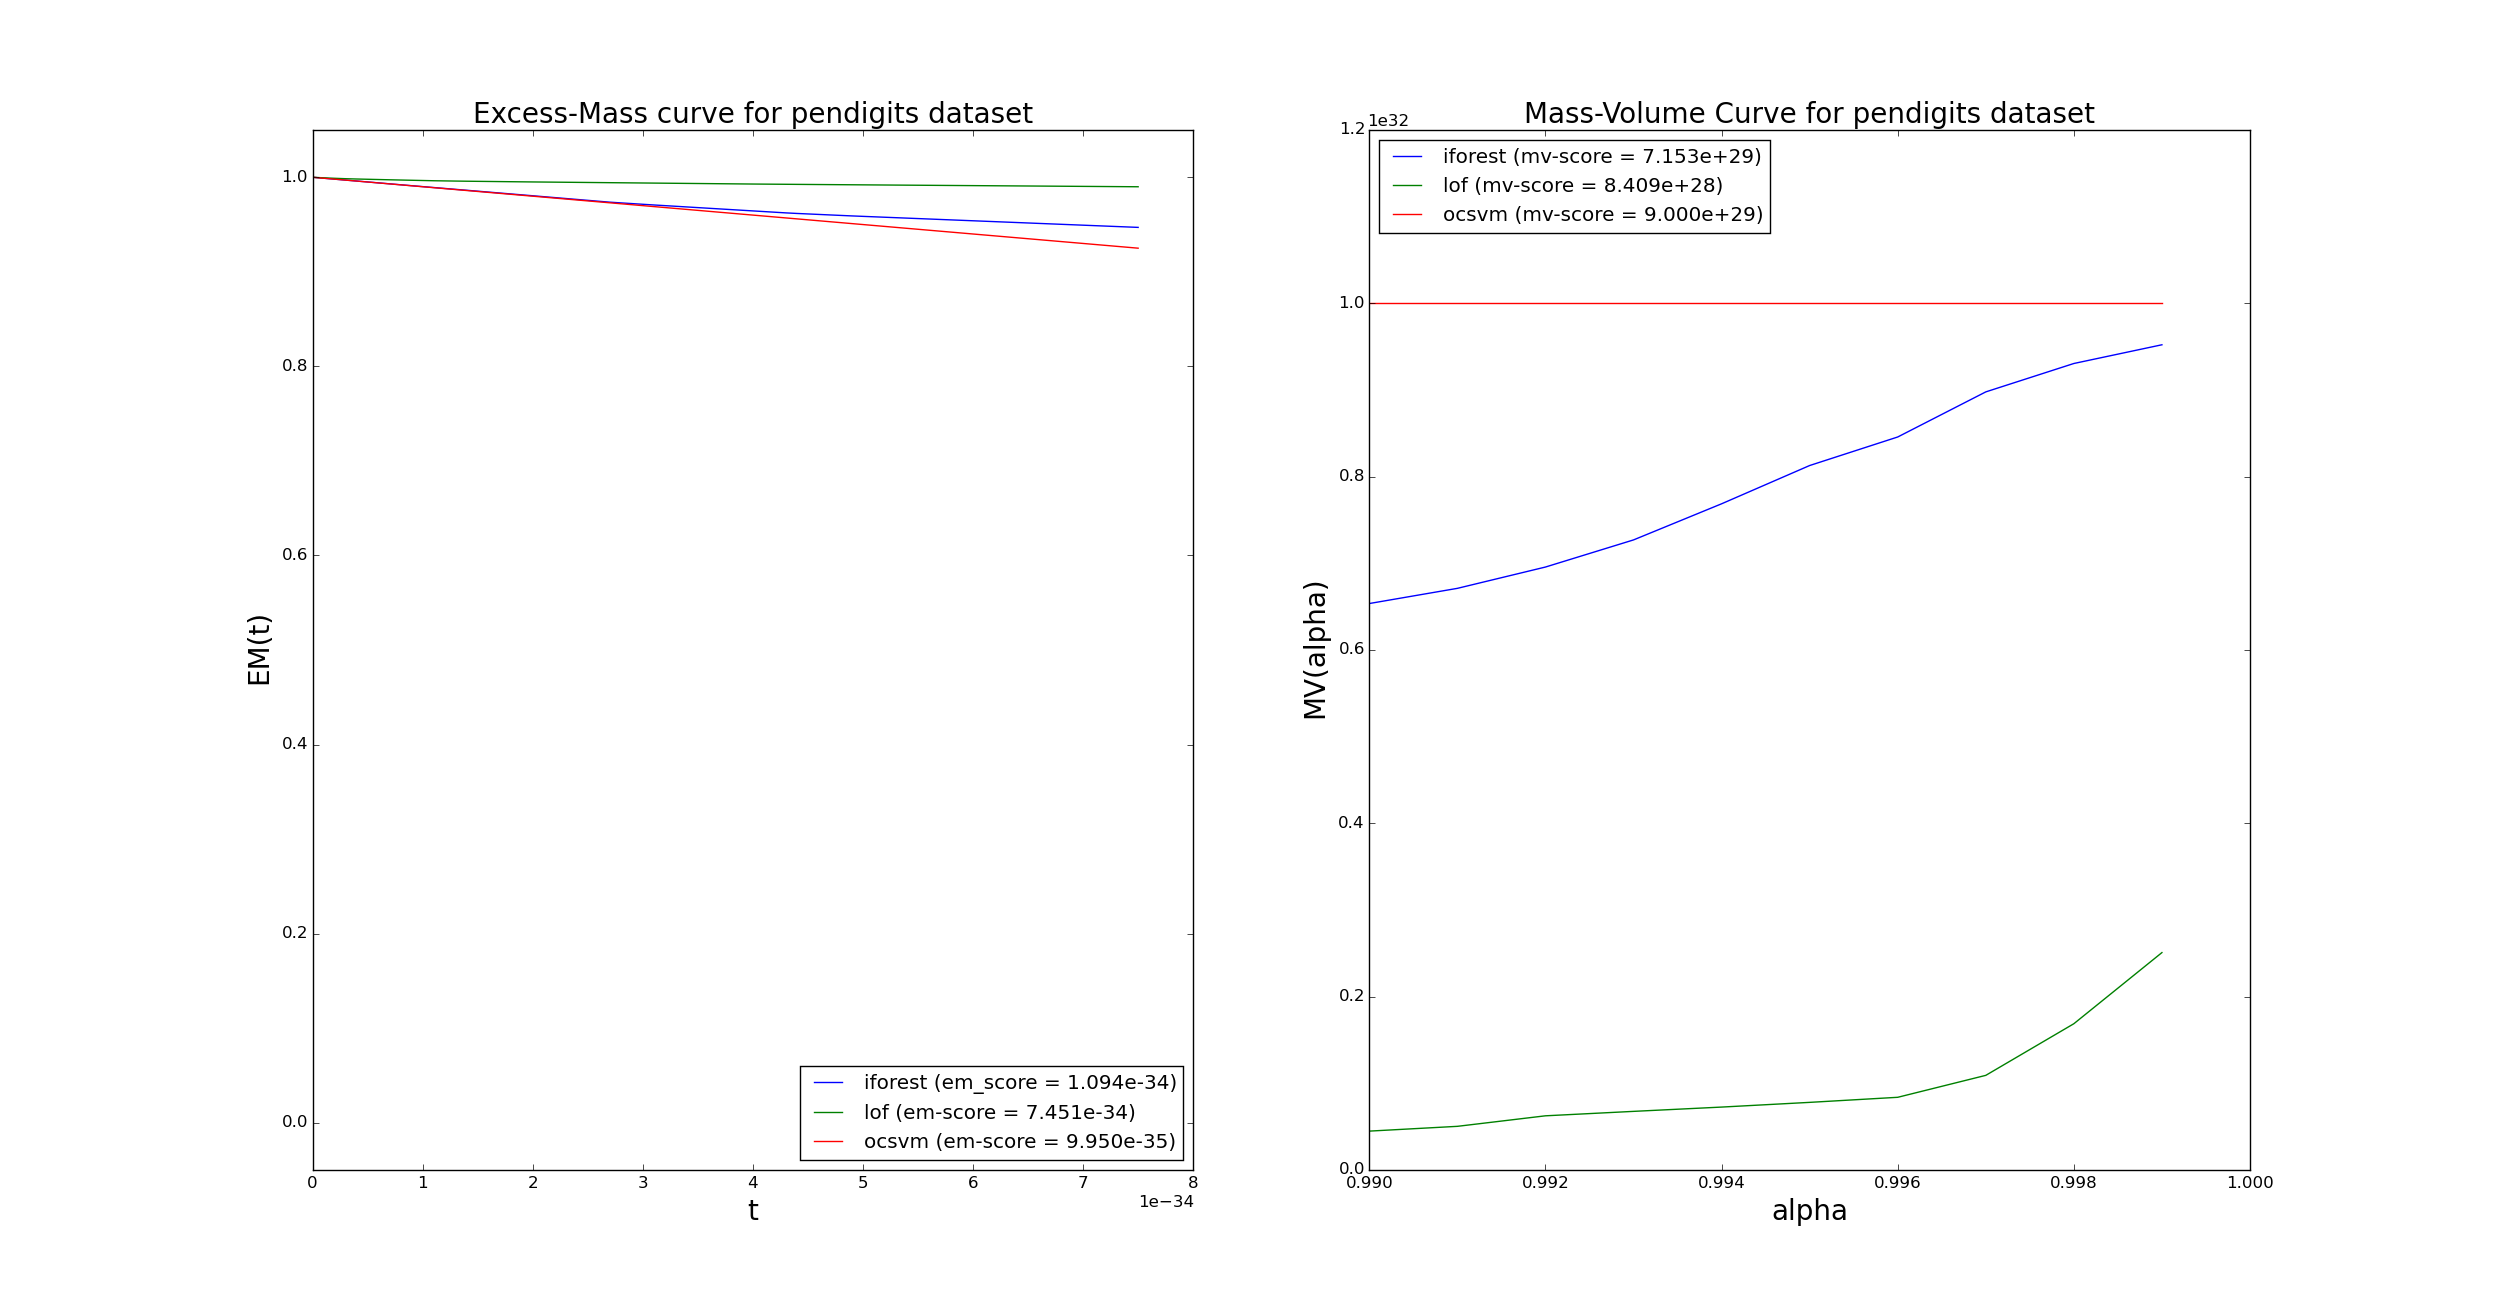
\includegraphics[trim=172 52 165 70, clip, width=\linewidth]{fig_source/evaluation_fig/t_mv_em_pendigits_unsupervised.png}
%   \caption{MV and EM curves for pendigits dataset (unsupervised framework)}
% \end{figure}

\begin{figure}[!ht]
\label{evaluation:mv_em_pima}
  \centering
  \caption{MV and EM curves for pima dataset (novelty detection framework)}
  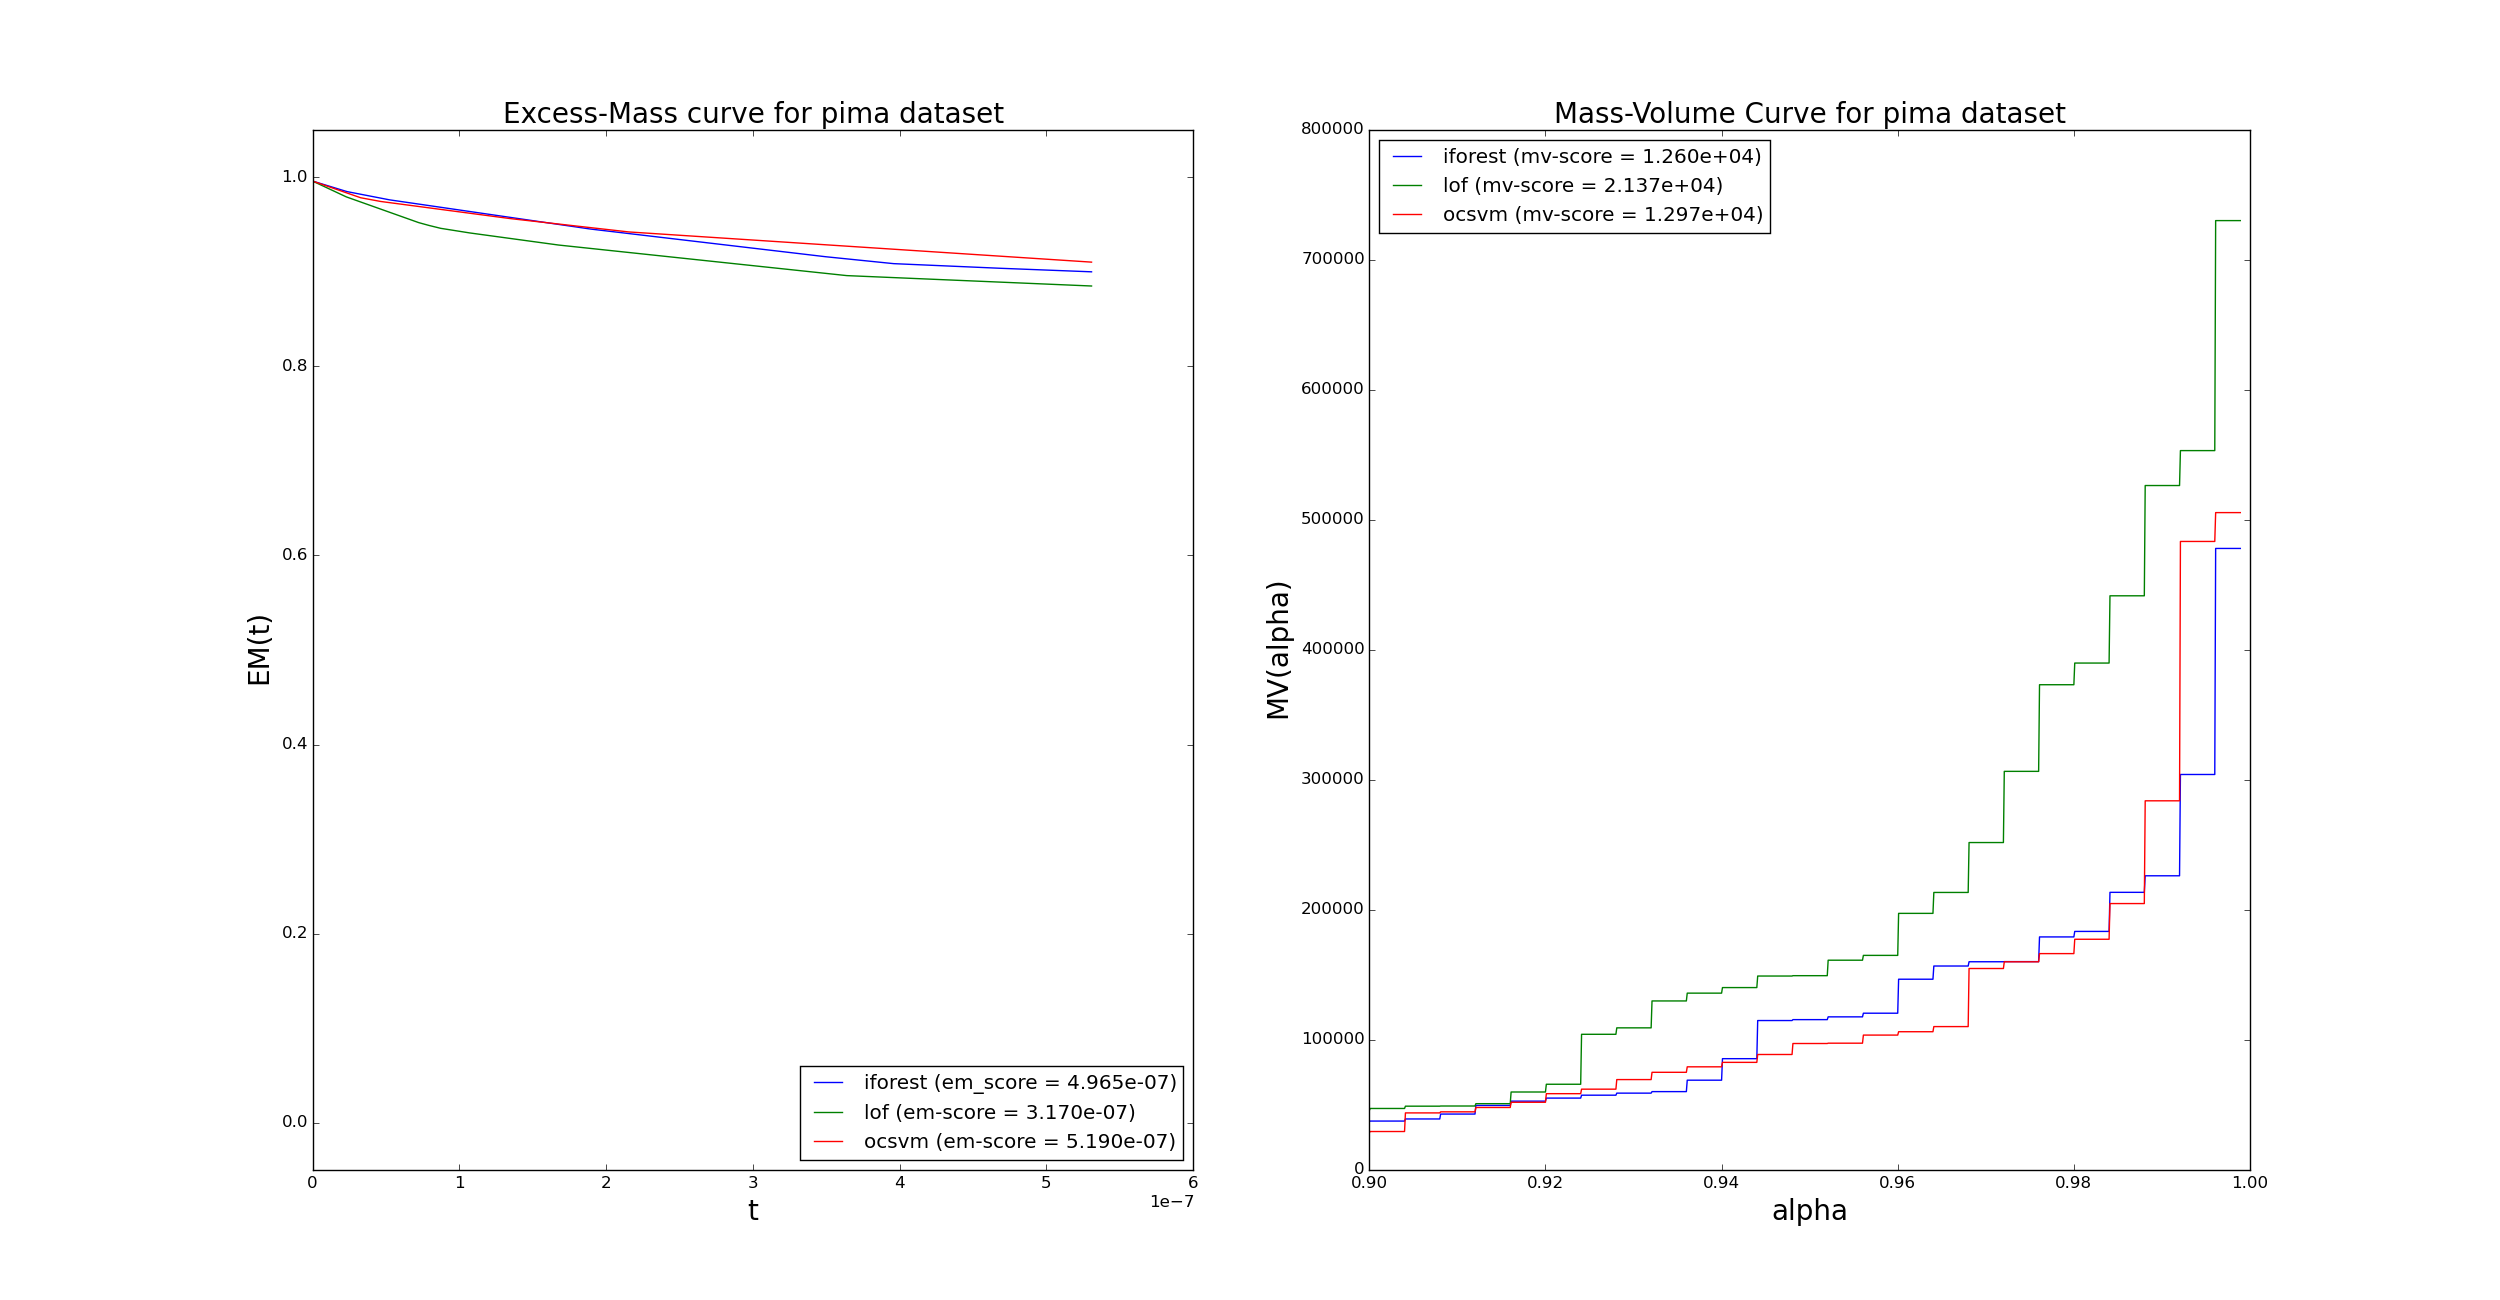
\includegraphics[trim=172 52 165 70, clip, width=\linewidth]{fig_source/evaluation_fig/mv_em_pima_supervised_09_factorized.png}
\end{figure}
\begin{figure}[!ht]
\label{evaluation:mv_em_pima_unsupervised}
  \centering
  \caption{MV and EM curves for pima dataset (unsupervised framework)}
  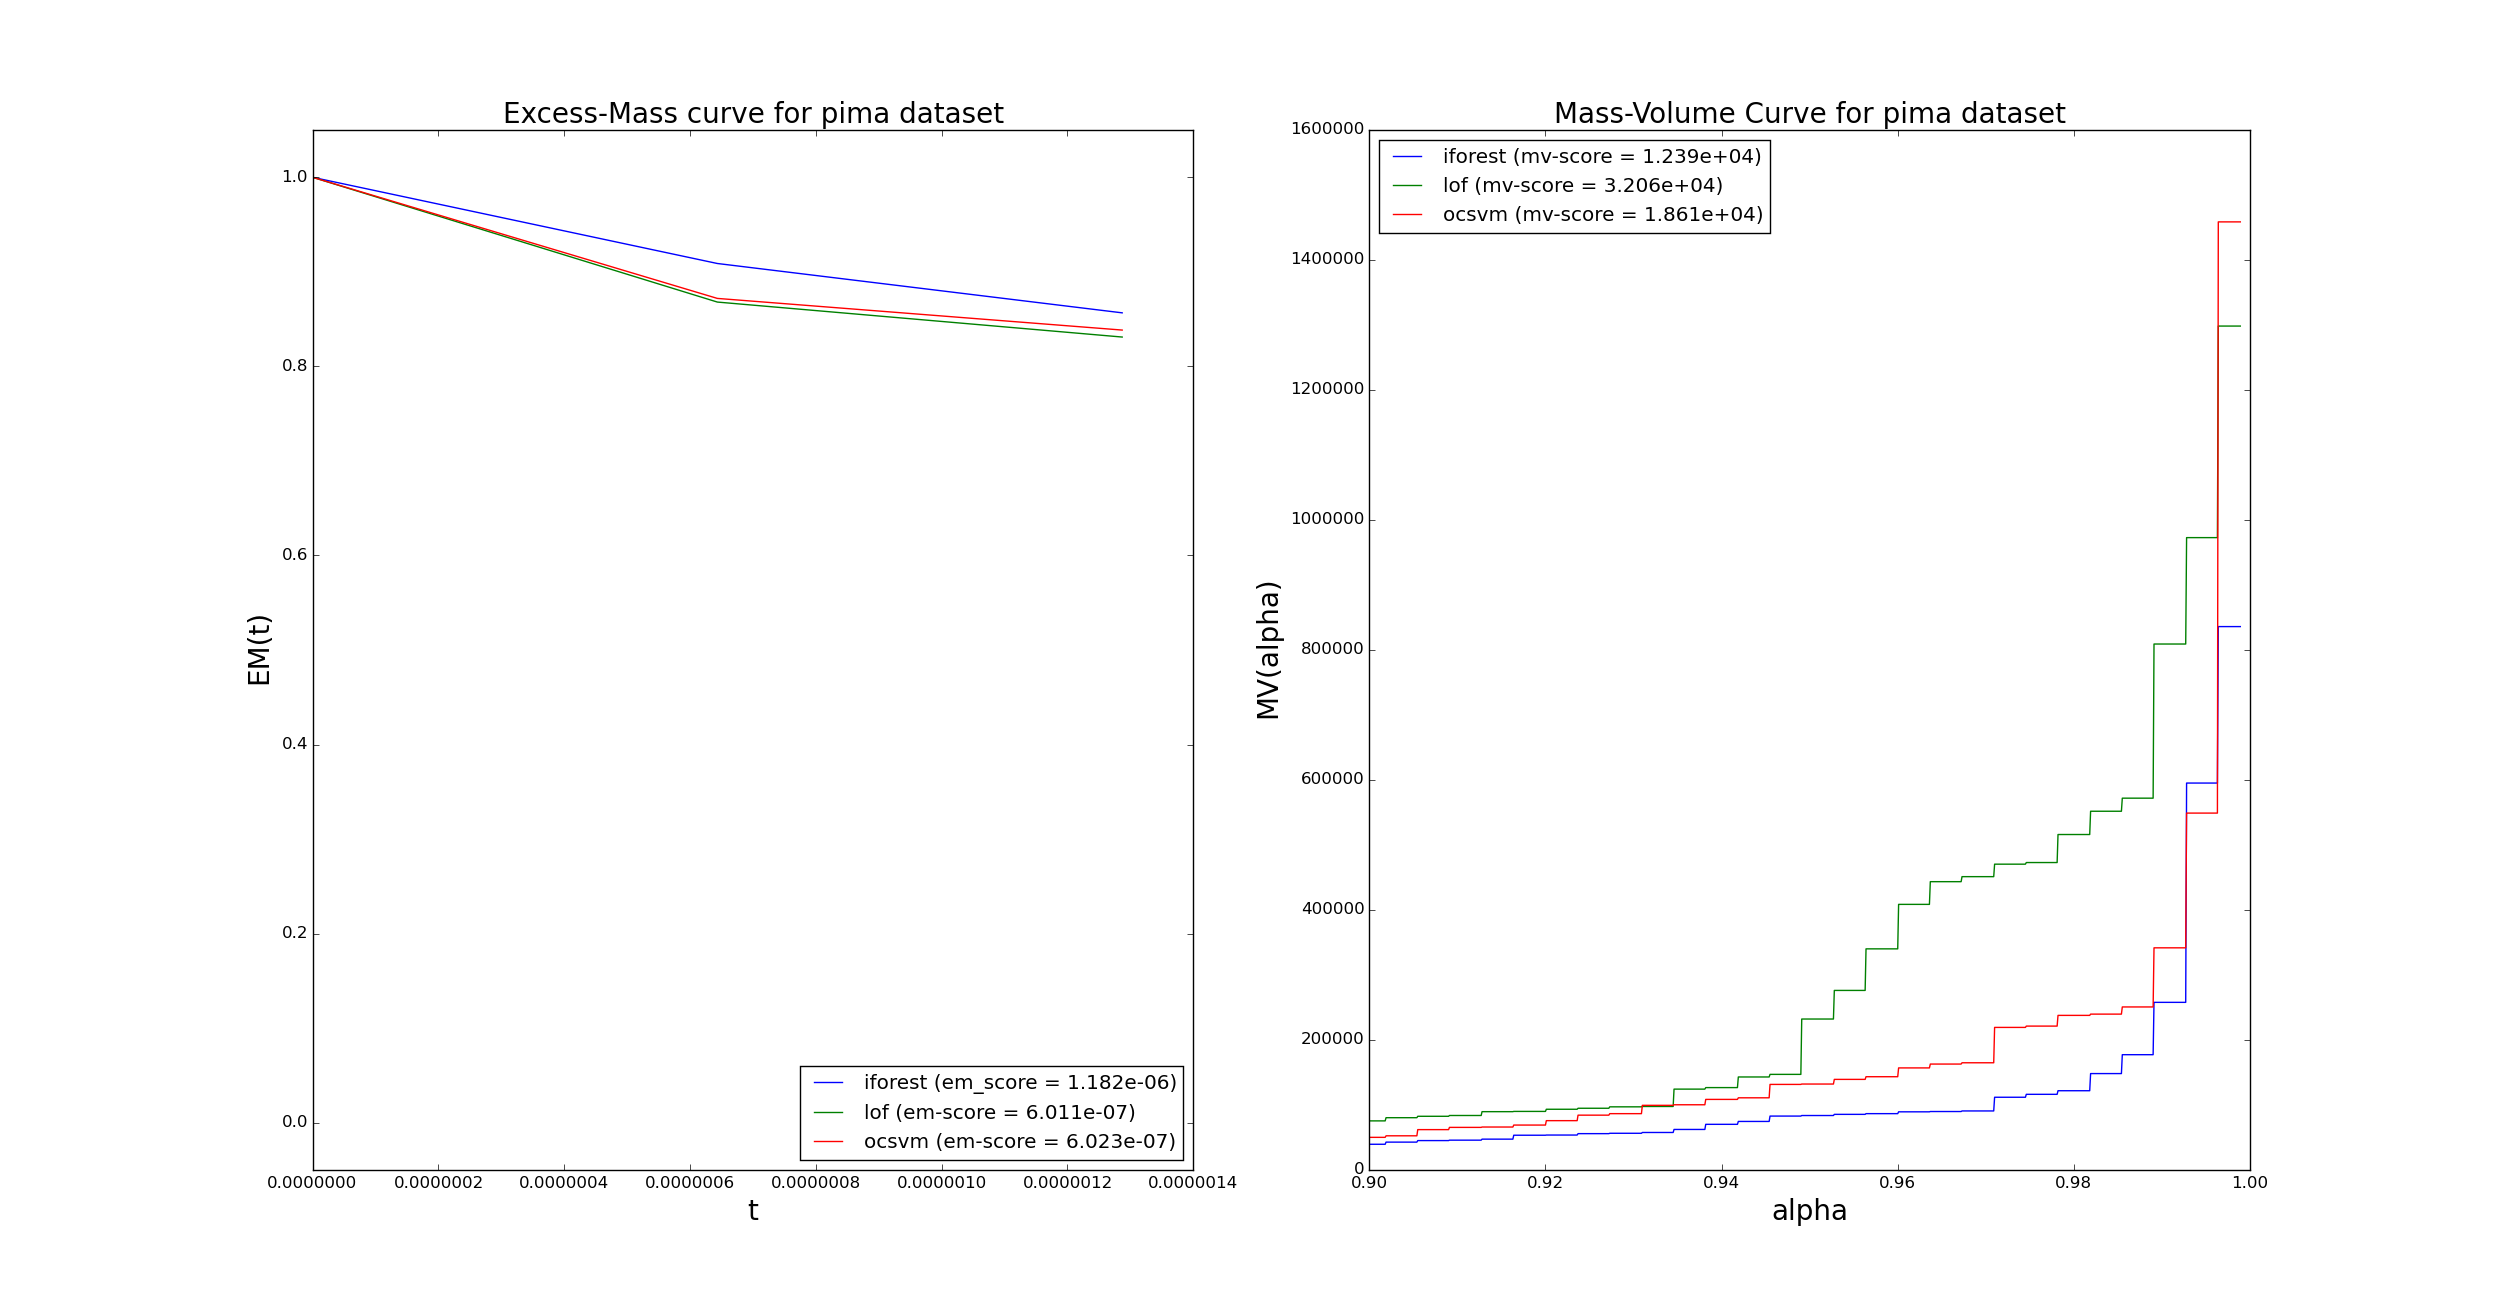
\includegraphics[trim=172 52 165 70, clip, width=\linewidth]{fig_source/evaluation_fig/mv_em_pima_unsupervised_09_factorized.png}
\end{figure}

\begin{figure}[!ht]
\label{evaluation:mv_em_smtp}
  \centering
  \caption{MV and EM curves for smtp dataset (novelty detection framework)}
  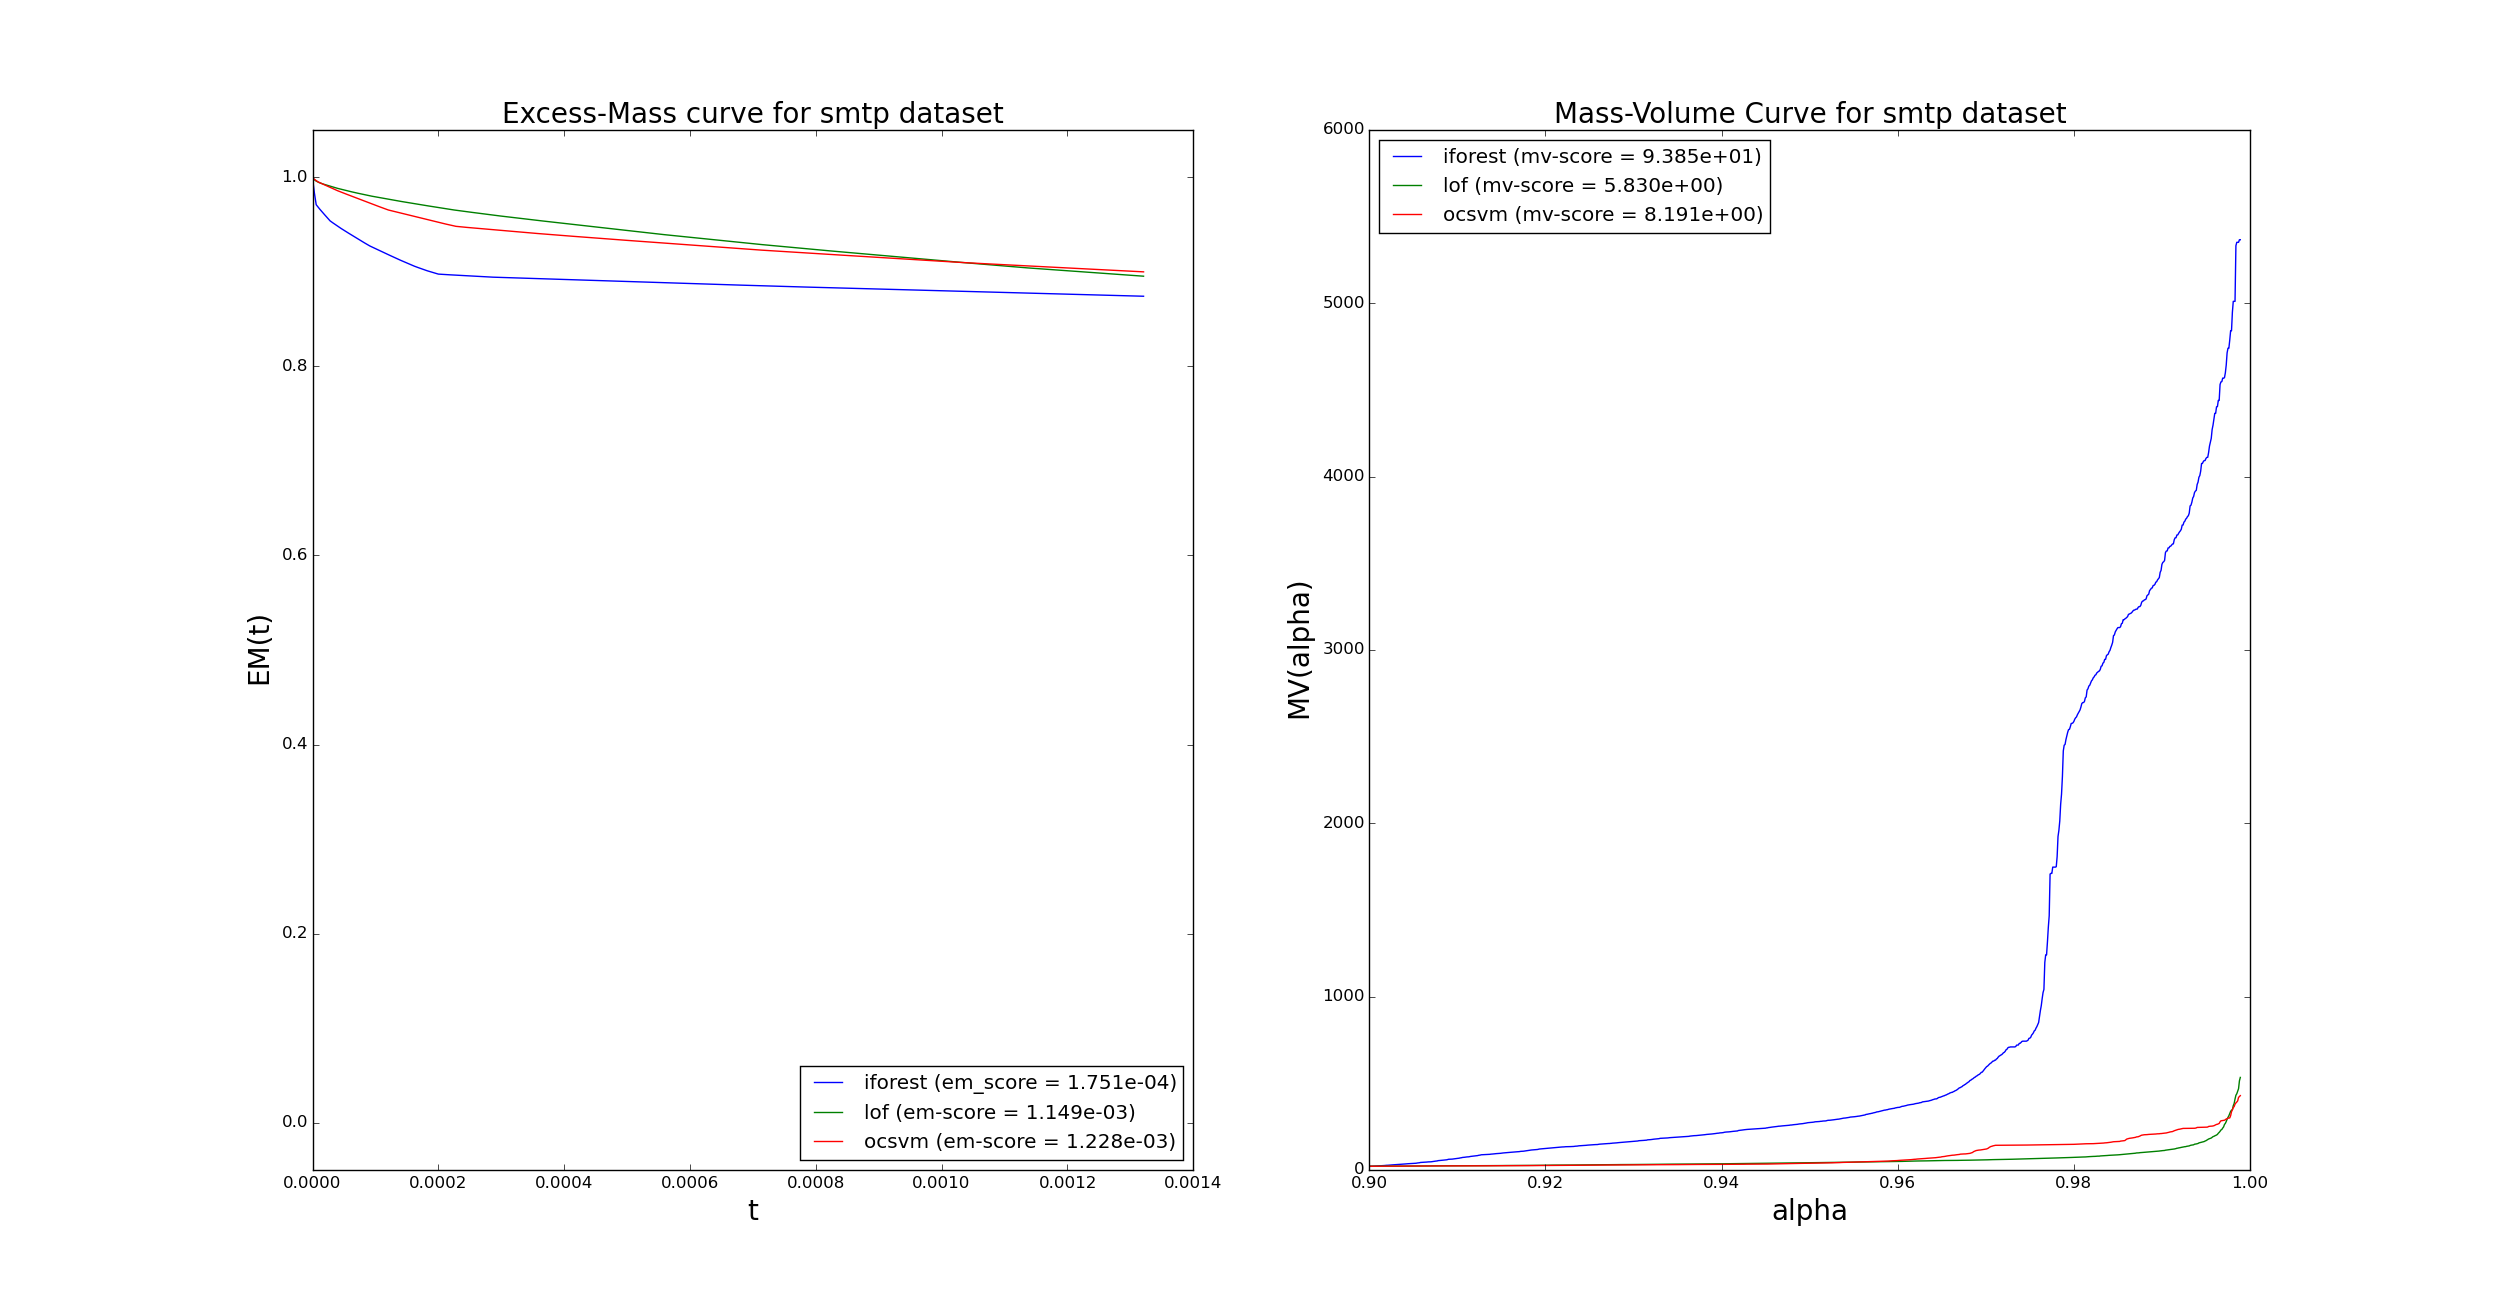
\includegraphics[trim=172 52 165 70, clip, width=\linewidth]{fig_source/evaluation_fig/mv_em_smtp_supervised_09_factorized.png}
\end{figure}
\begin{figure}[!ht]
\label{evaluation:mv_em_smtp_unsupervised}
  \centering
  \caption{MV and EM curves for smtp dataset (unsupervised framework)}
  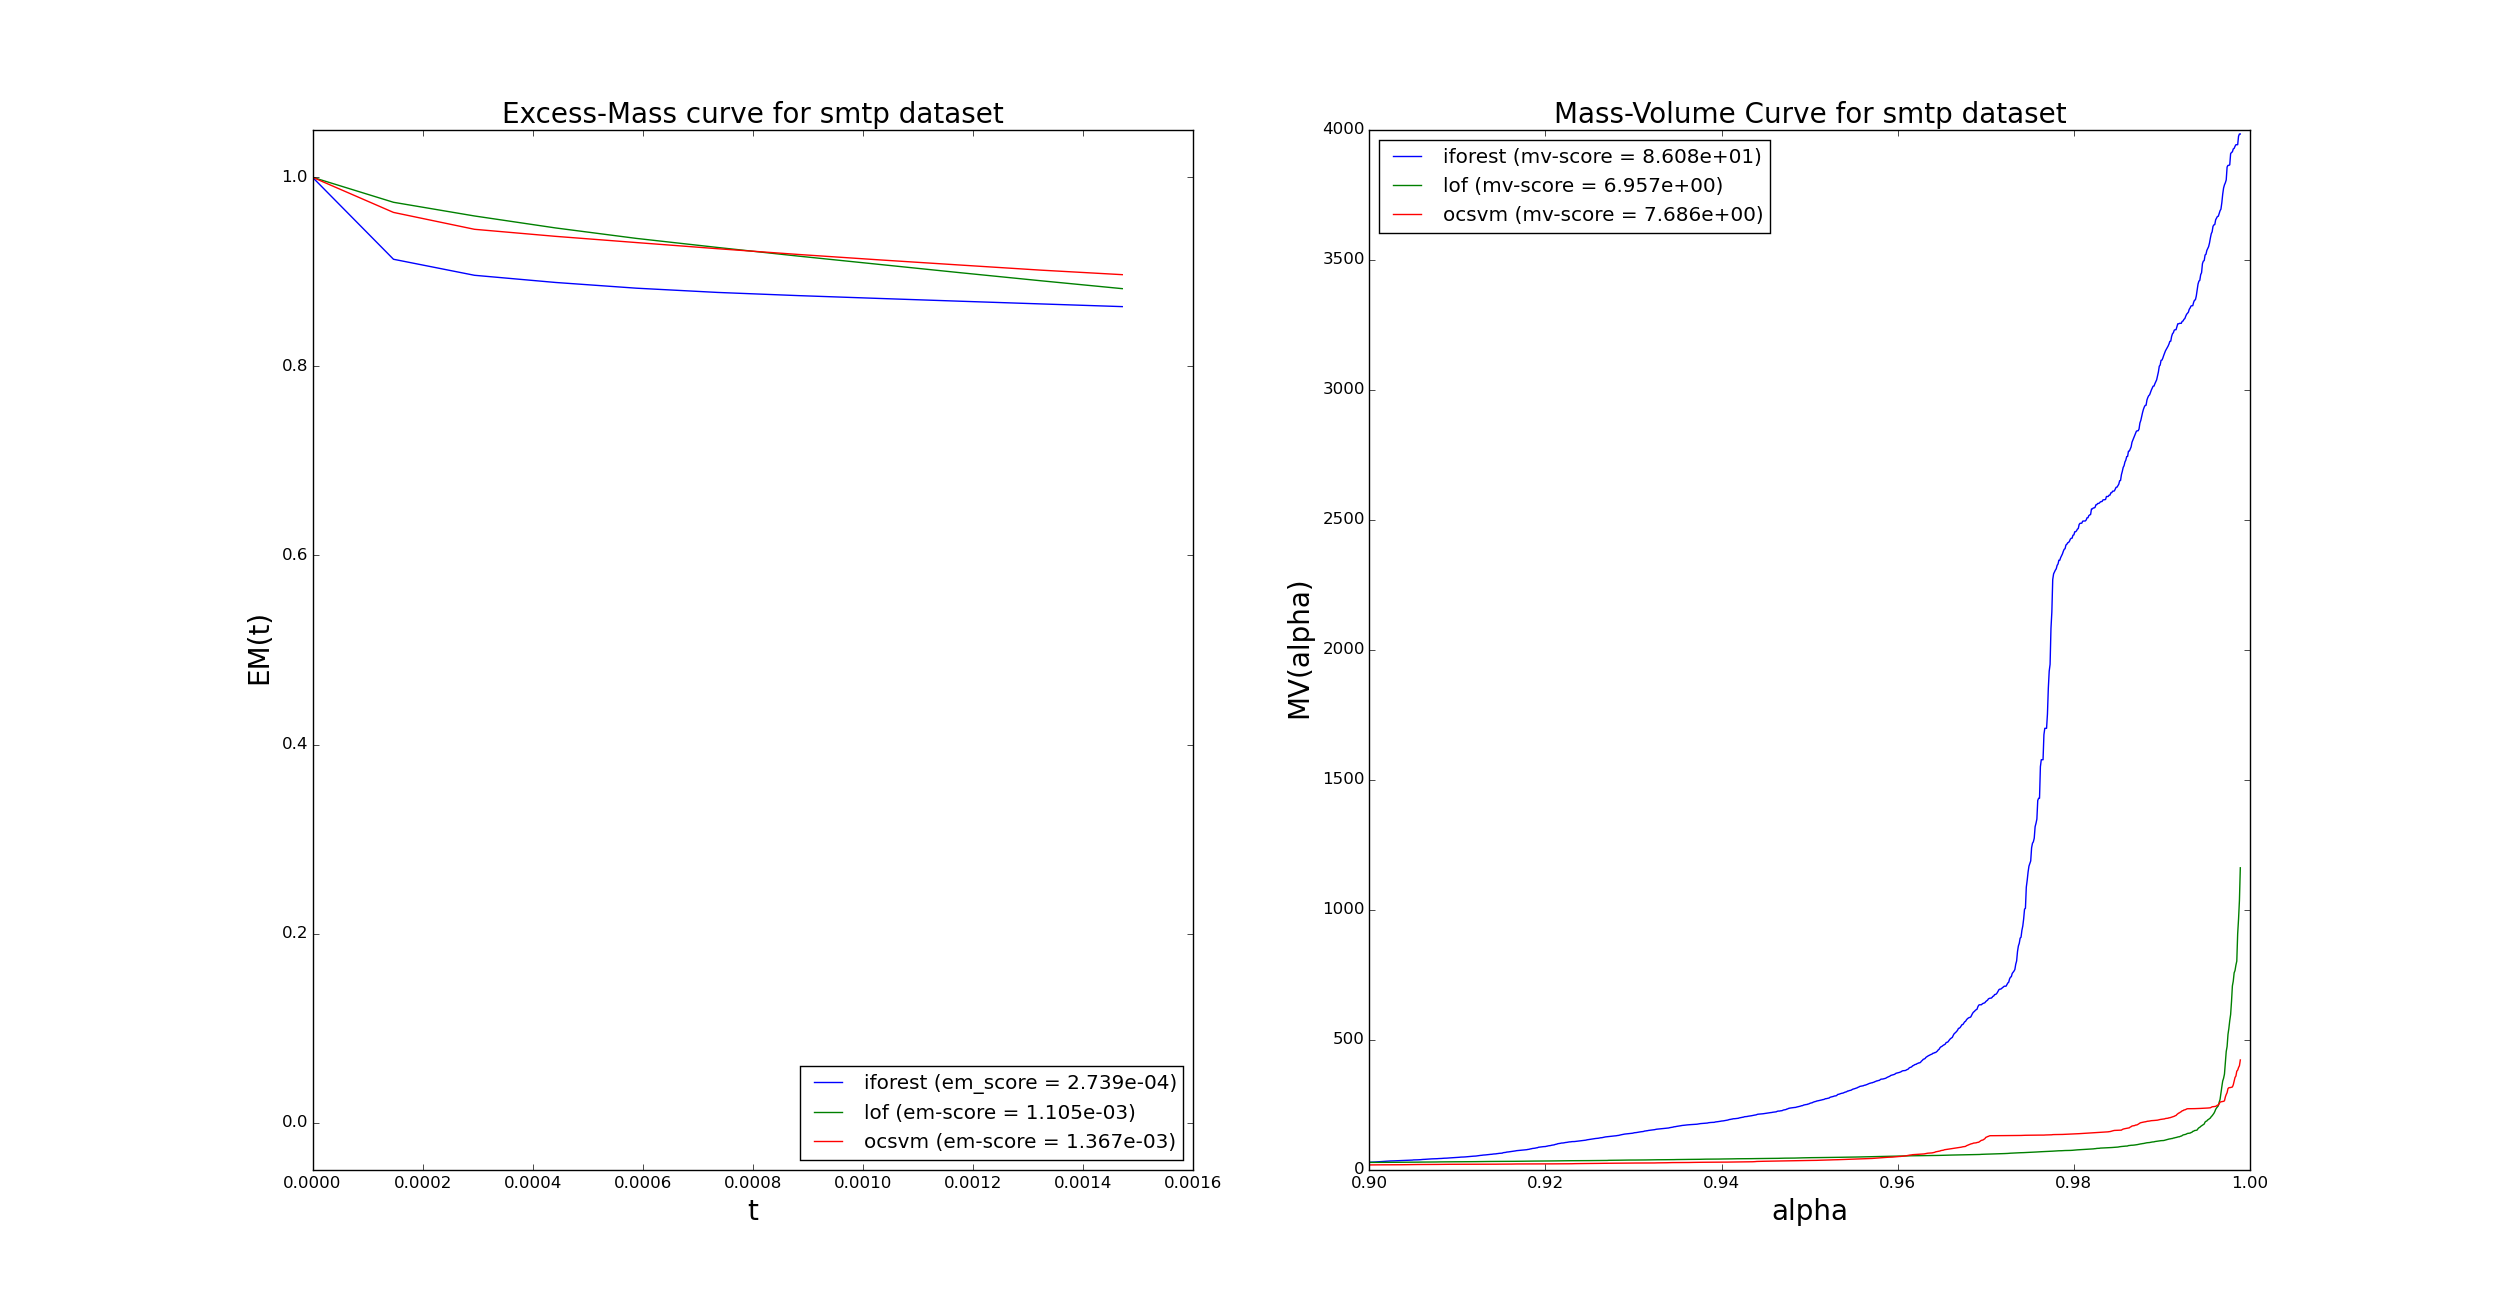
\includegraphics[trim=172 52 165 70, clip, width=\linewidth]{fig_source/evaluation_fig/mv_em_smtp_unsupervised_09_factorized.png}
\end{figure}

\begin{figure}[!ht]
\label{evaluation:mv_em_wilt}
  \centering
  \caption{MV and EM curves for wilt dataset (novelty detection framework)}
  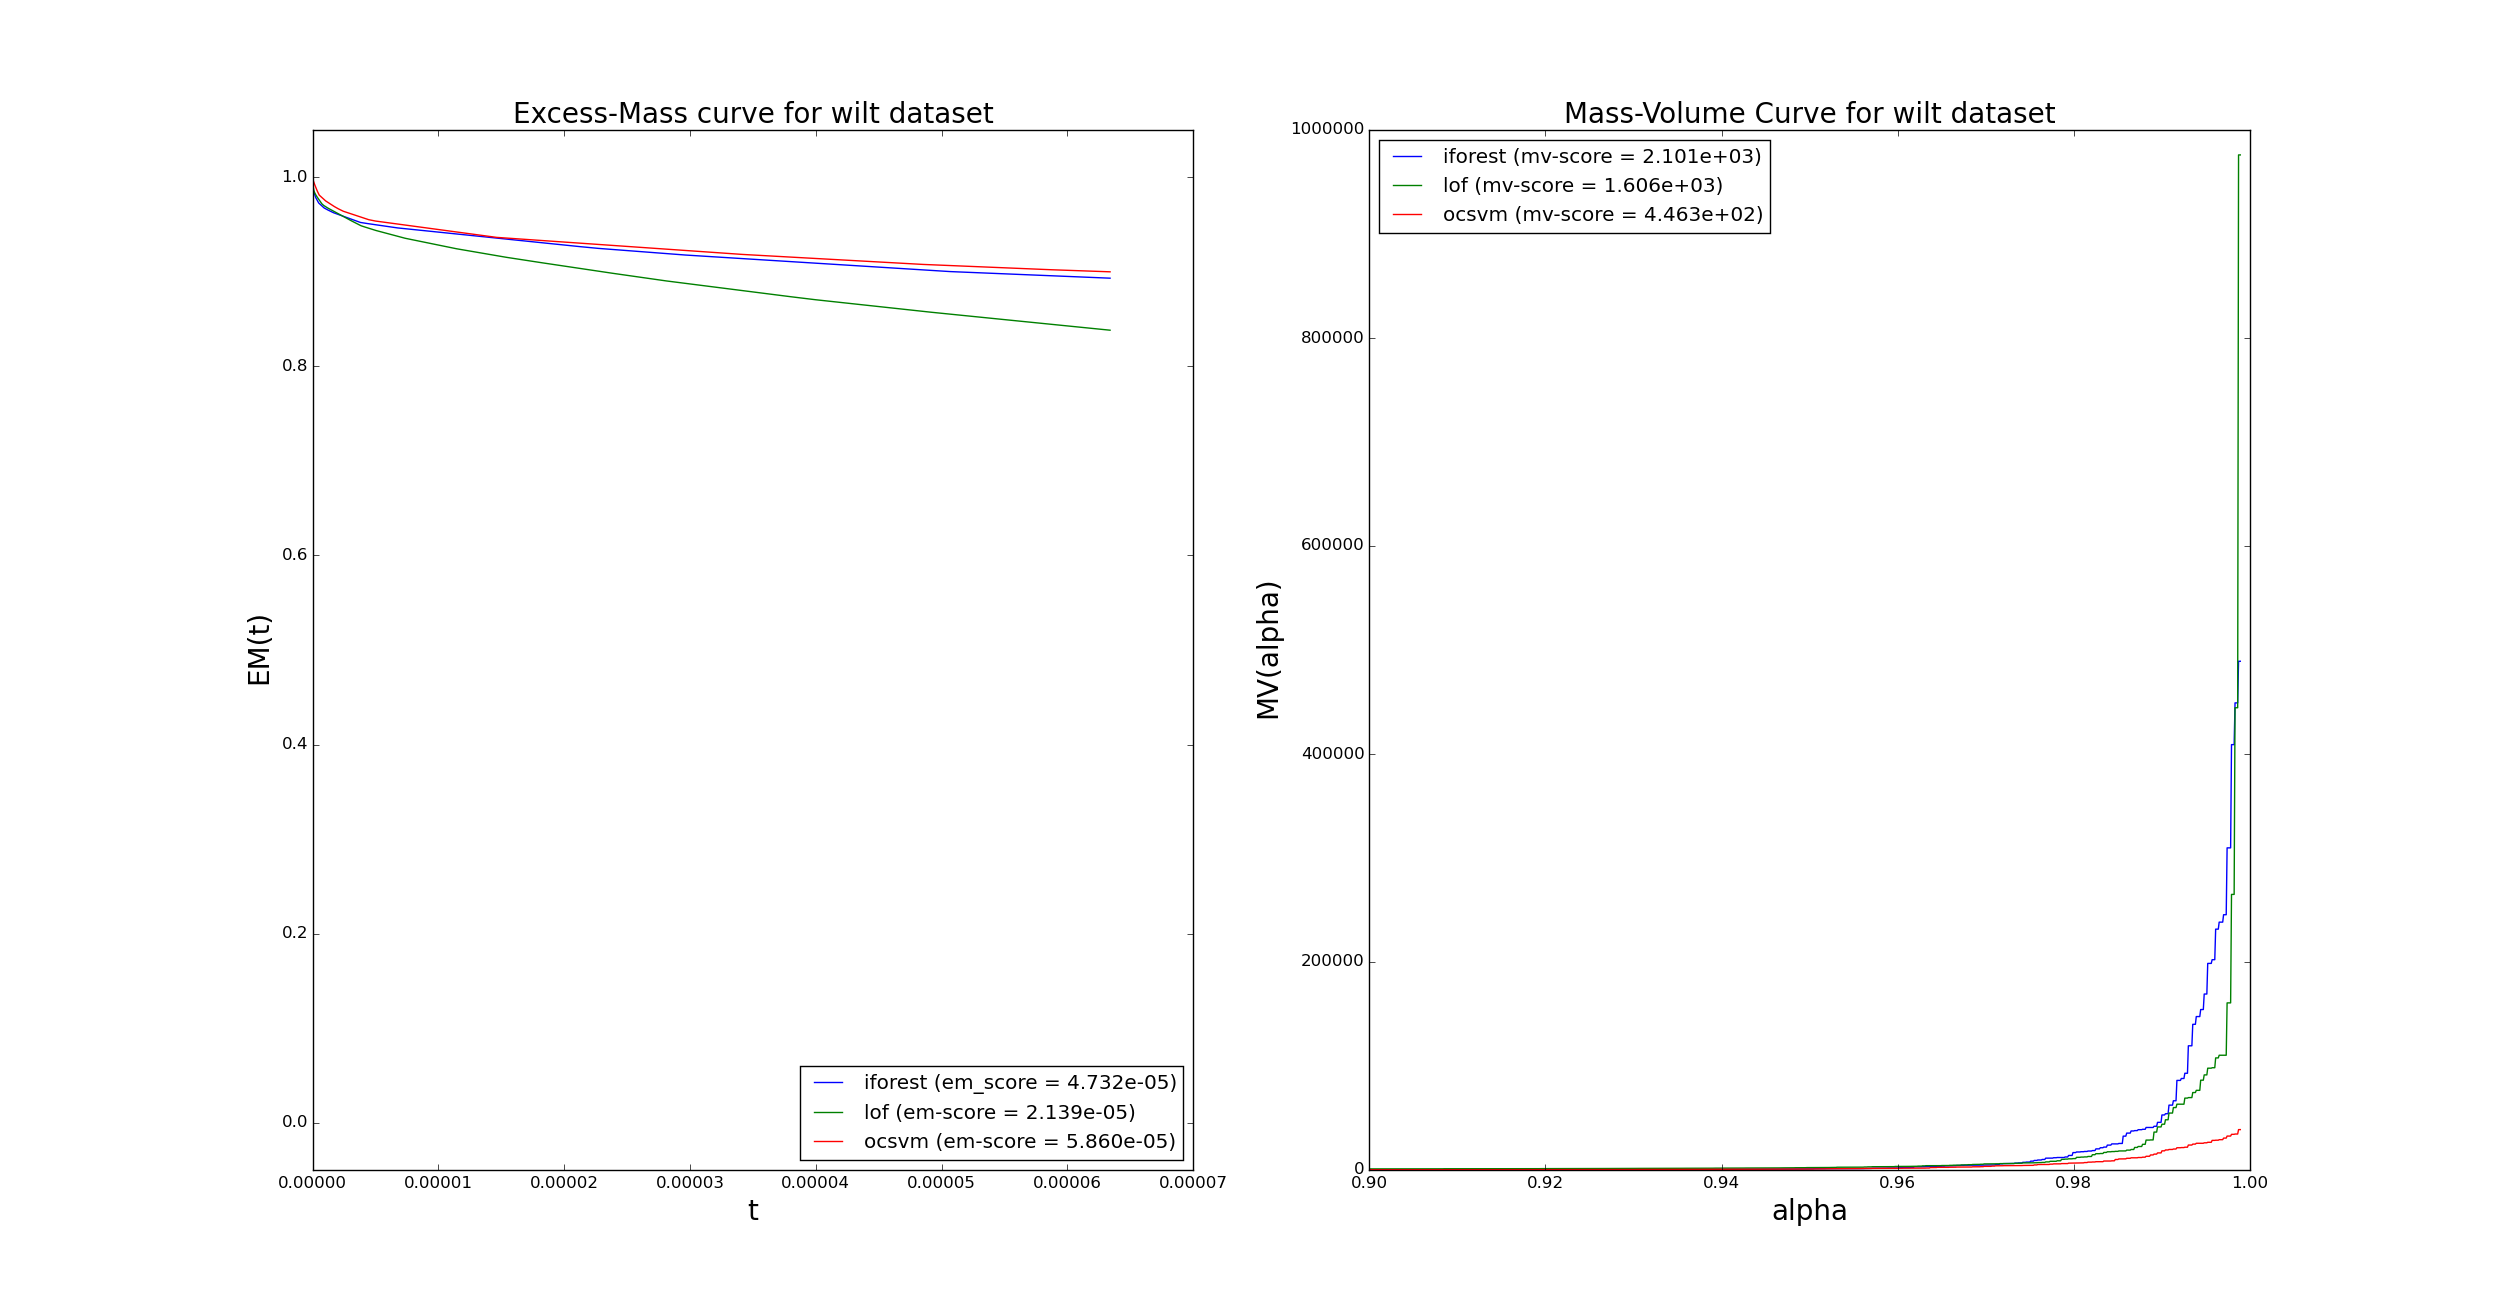
\includegraphics[trim=172 52 165 70, clip, width=\linewidth]{fig_source/evaluation_fig/mv_em_wilt_supervised_09_factorized.png}
\end{figure}
\begin{figure}[!ht]
\label{evaluation:mv_em_wilt_unsupervised}
  \centering
  \caption{MV and EM curves for wilt dataset (unsupervised framework)}
  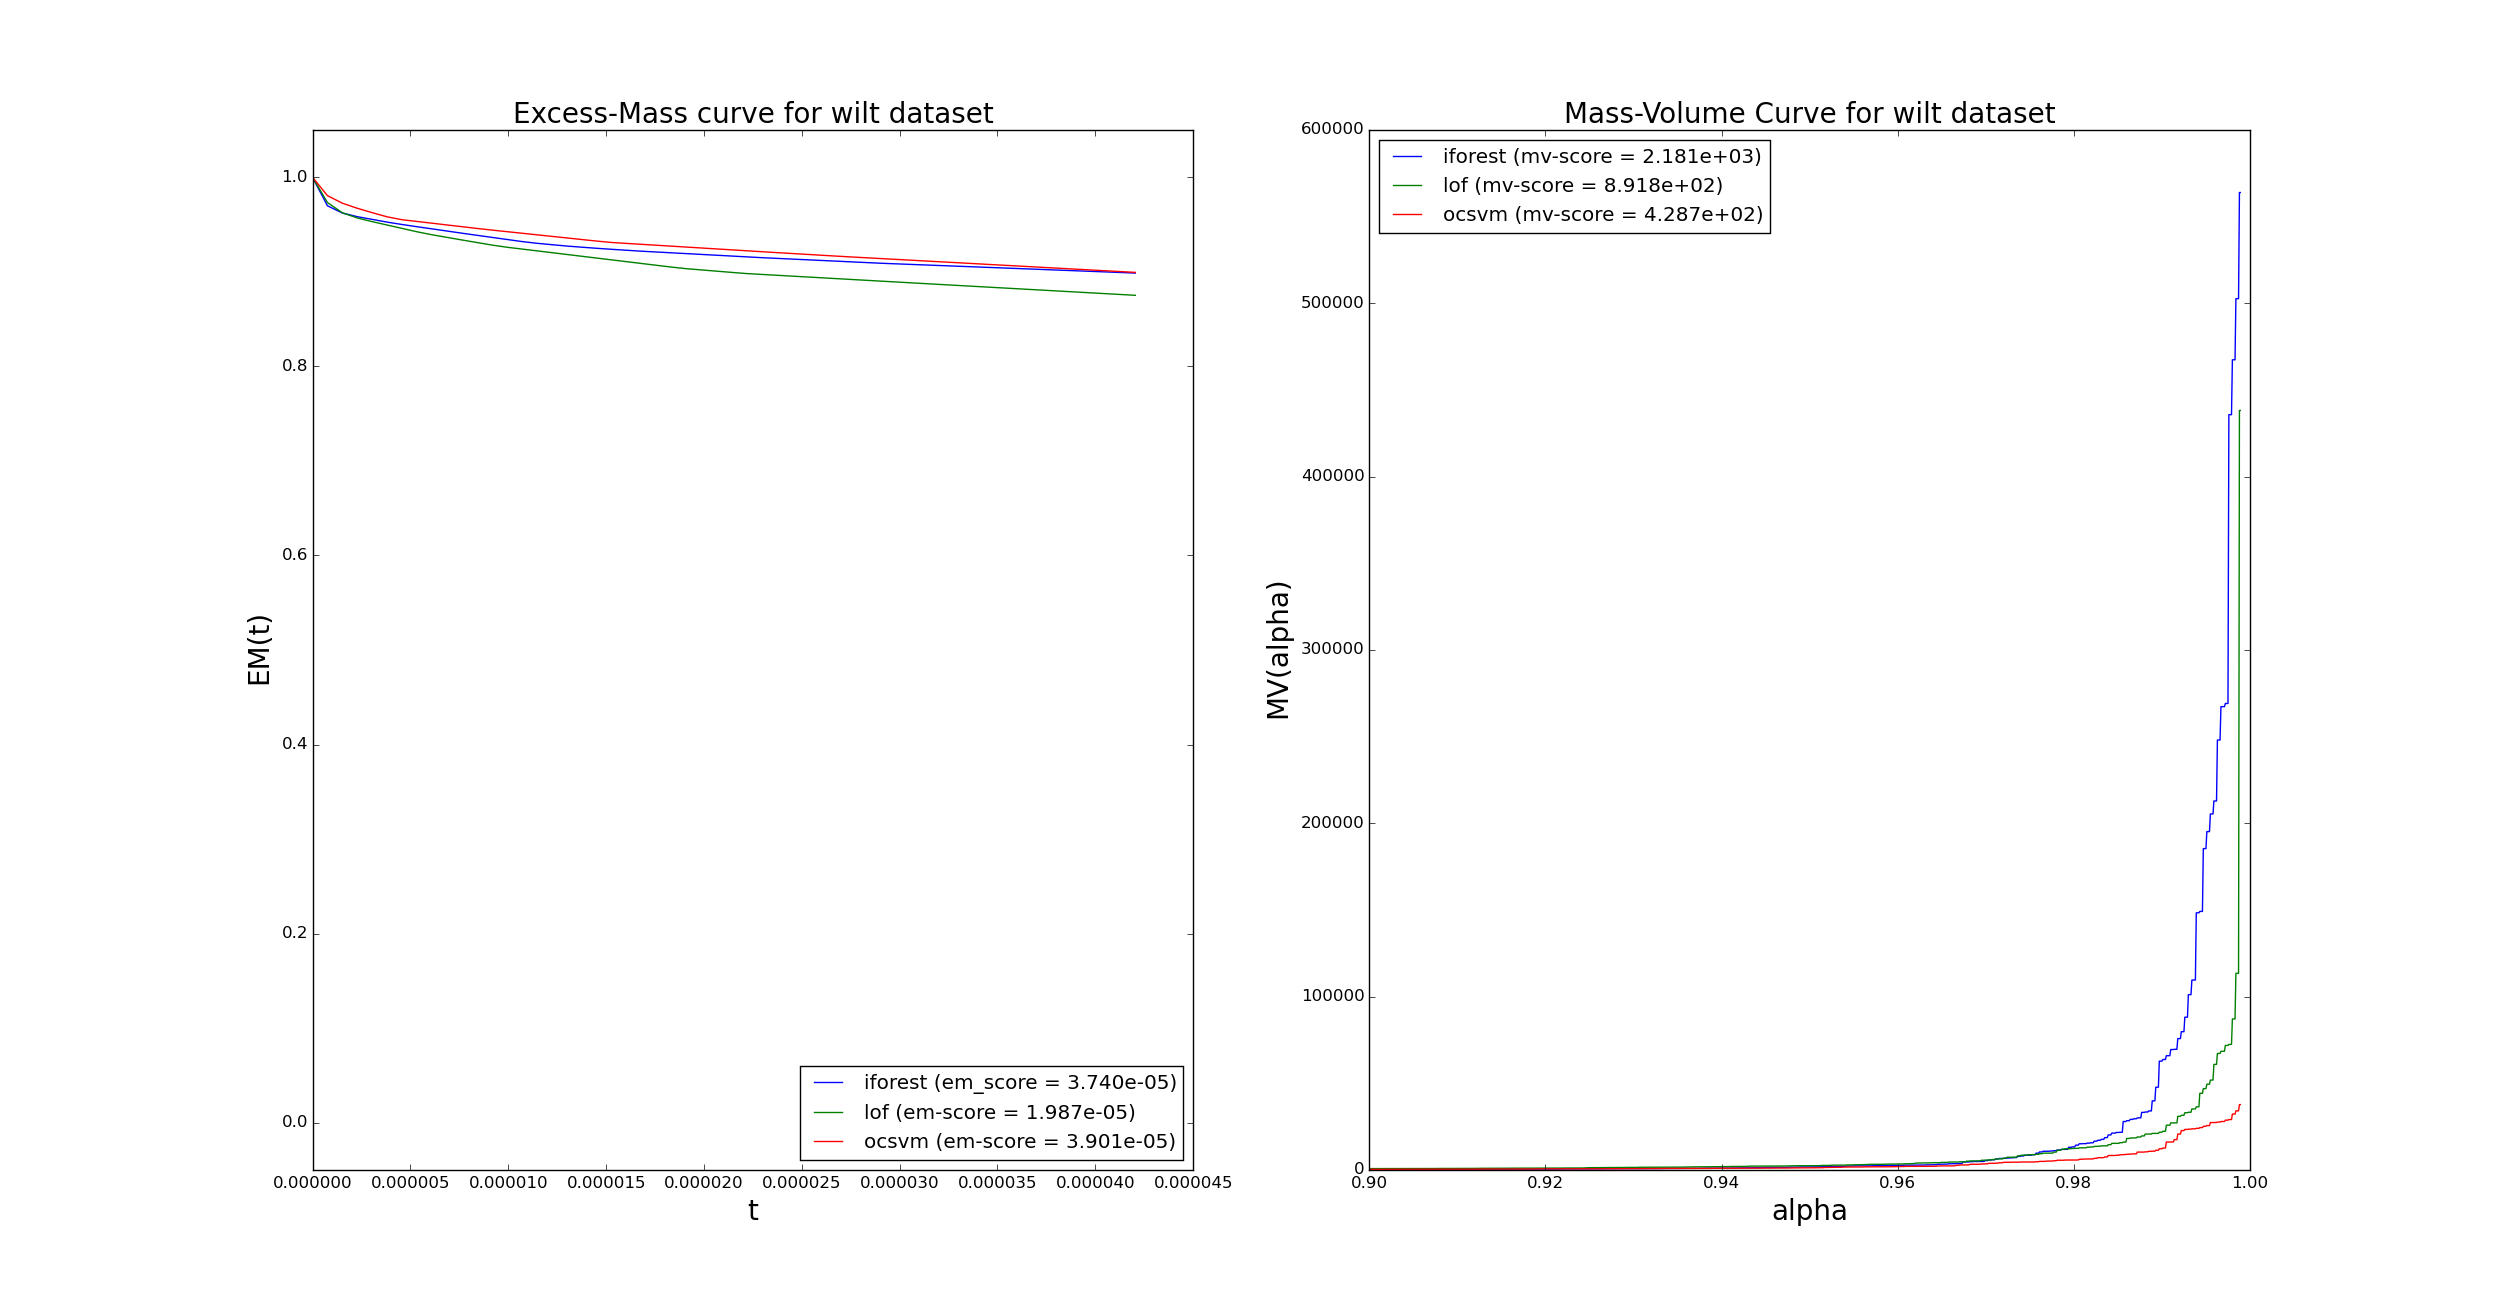
\includegraphics[trim=172 52 165 70, clip, width=\linewidth]{fig_source/evaluation_fig/mv_em_wilt_unsupervised_09_factorized.png}
\end{figure}



\begin{figure}[!ht]
  \centering
  \caption{MV and EM curves for adult dataset (novelty detection framework).}
  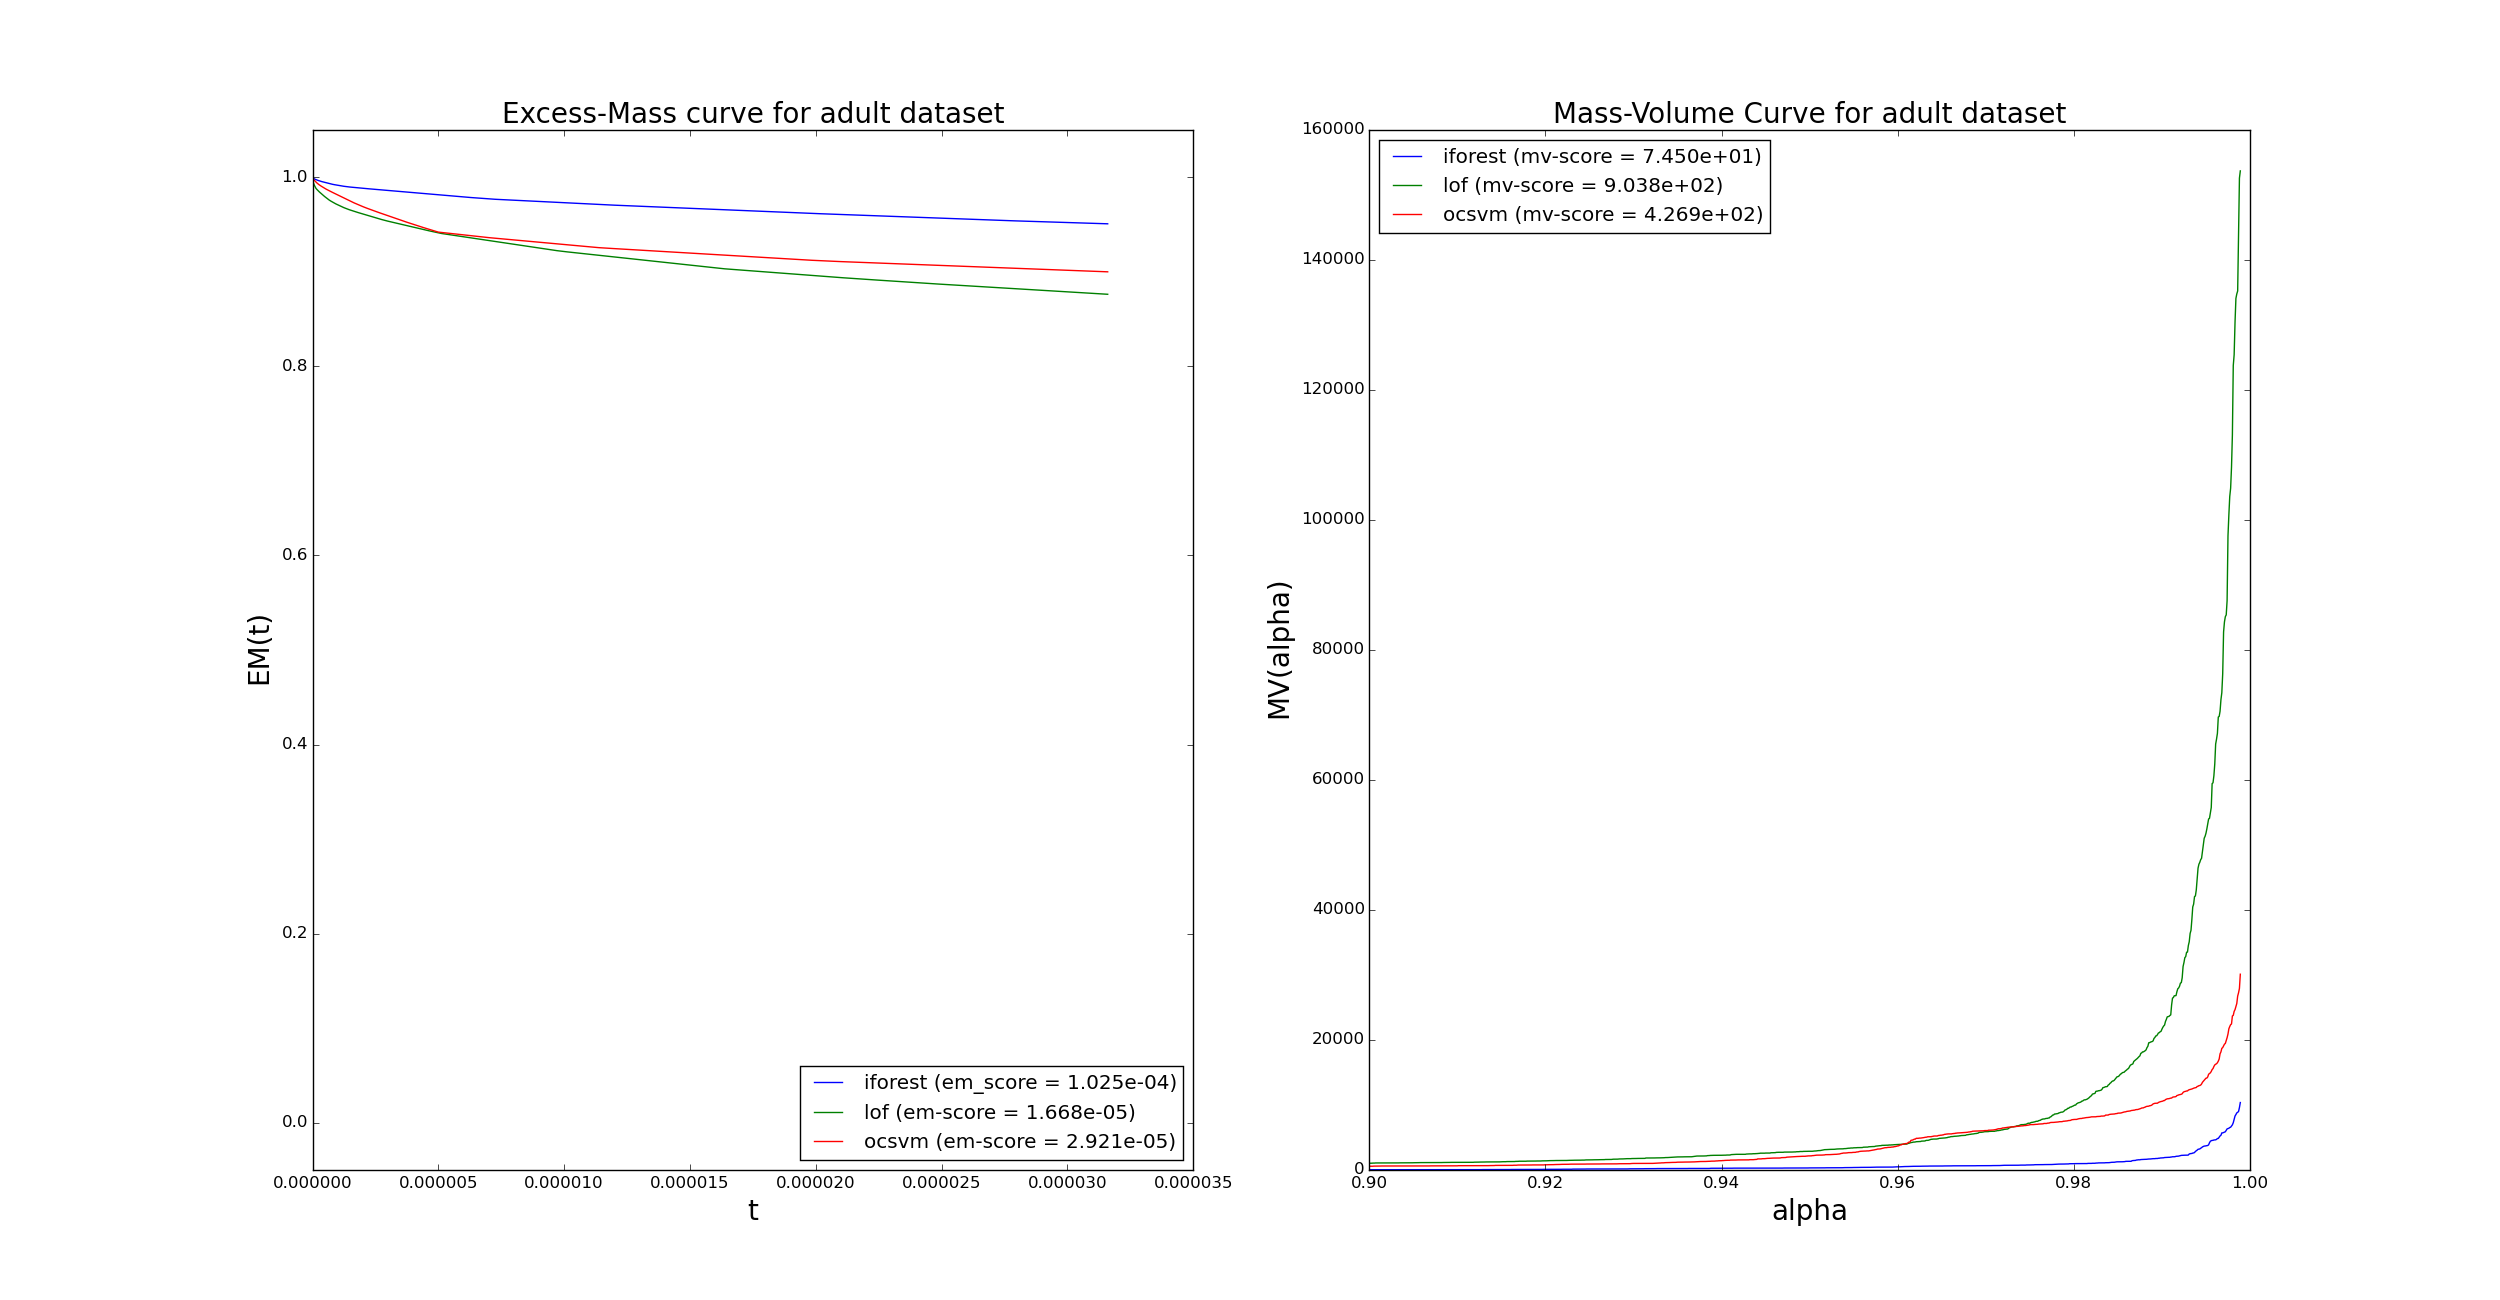
\includegraphics[trim=172 52 165 70, clip, width=\linewidth]{fig_source/evaluation_fig/mv_em_adult_supervised_09_factorized.png}
\end{figure}


\begin{figure}[!ht]
  \centering
  \caption{MV and EM curves for adult dataset (unsupervised framework)}
  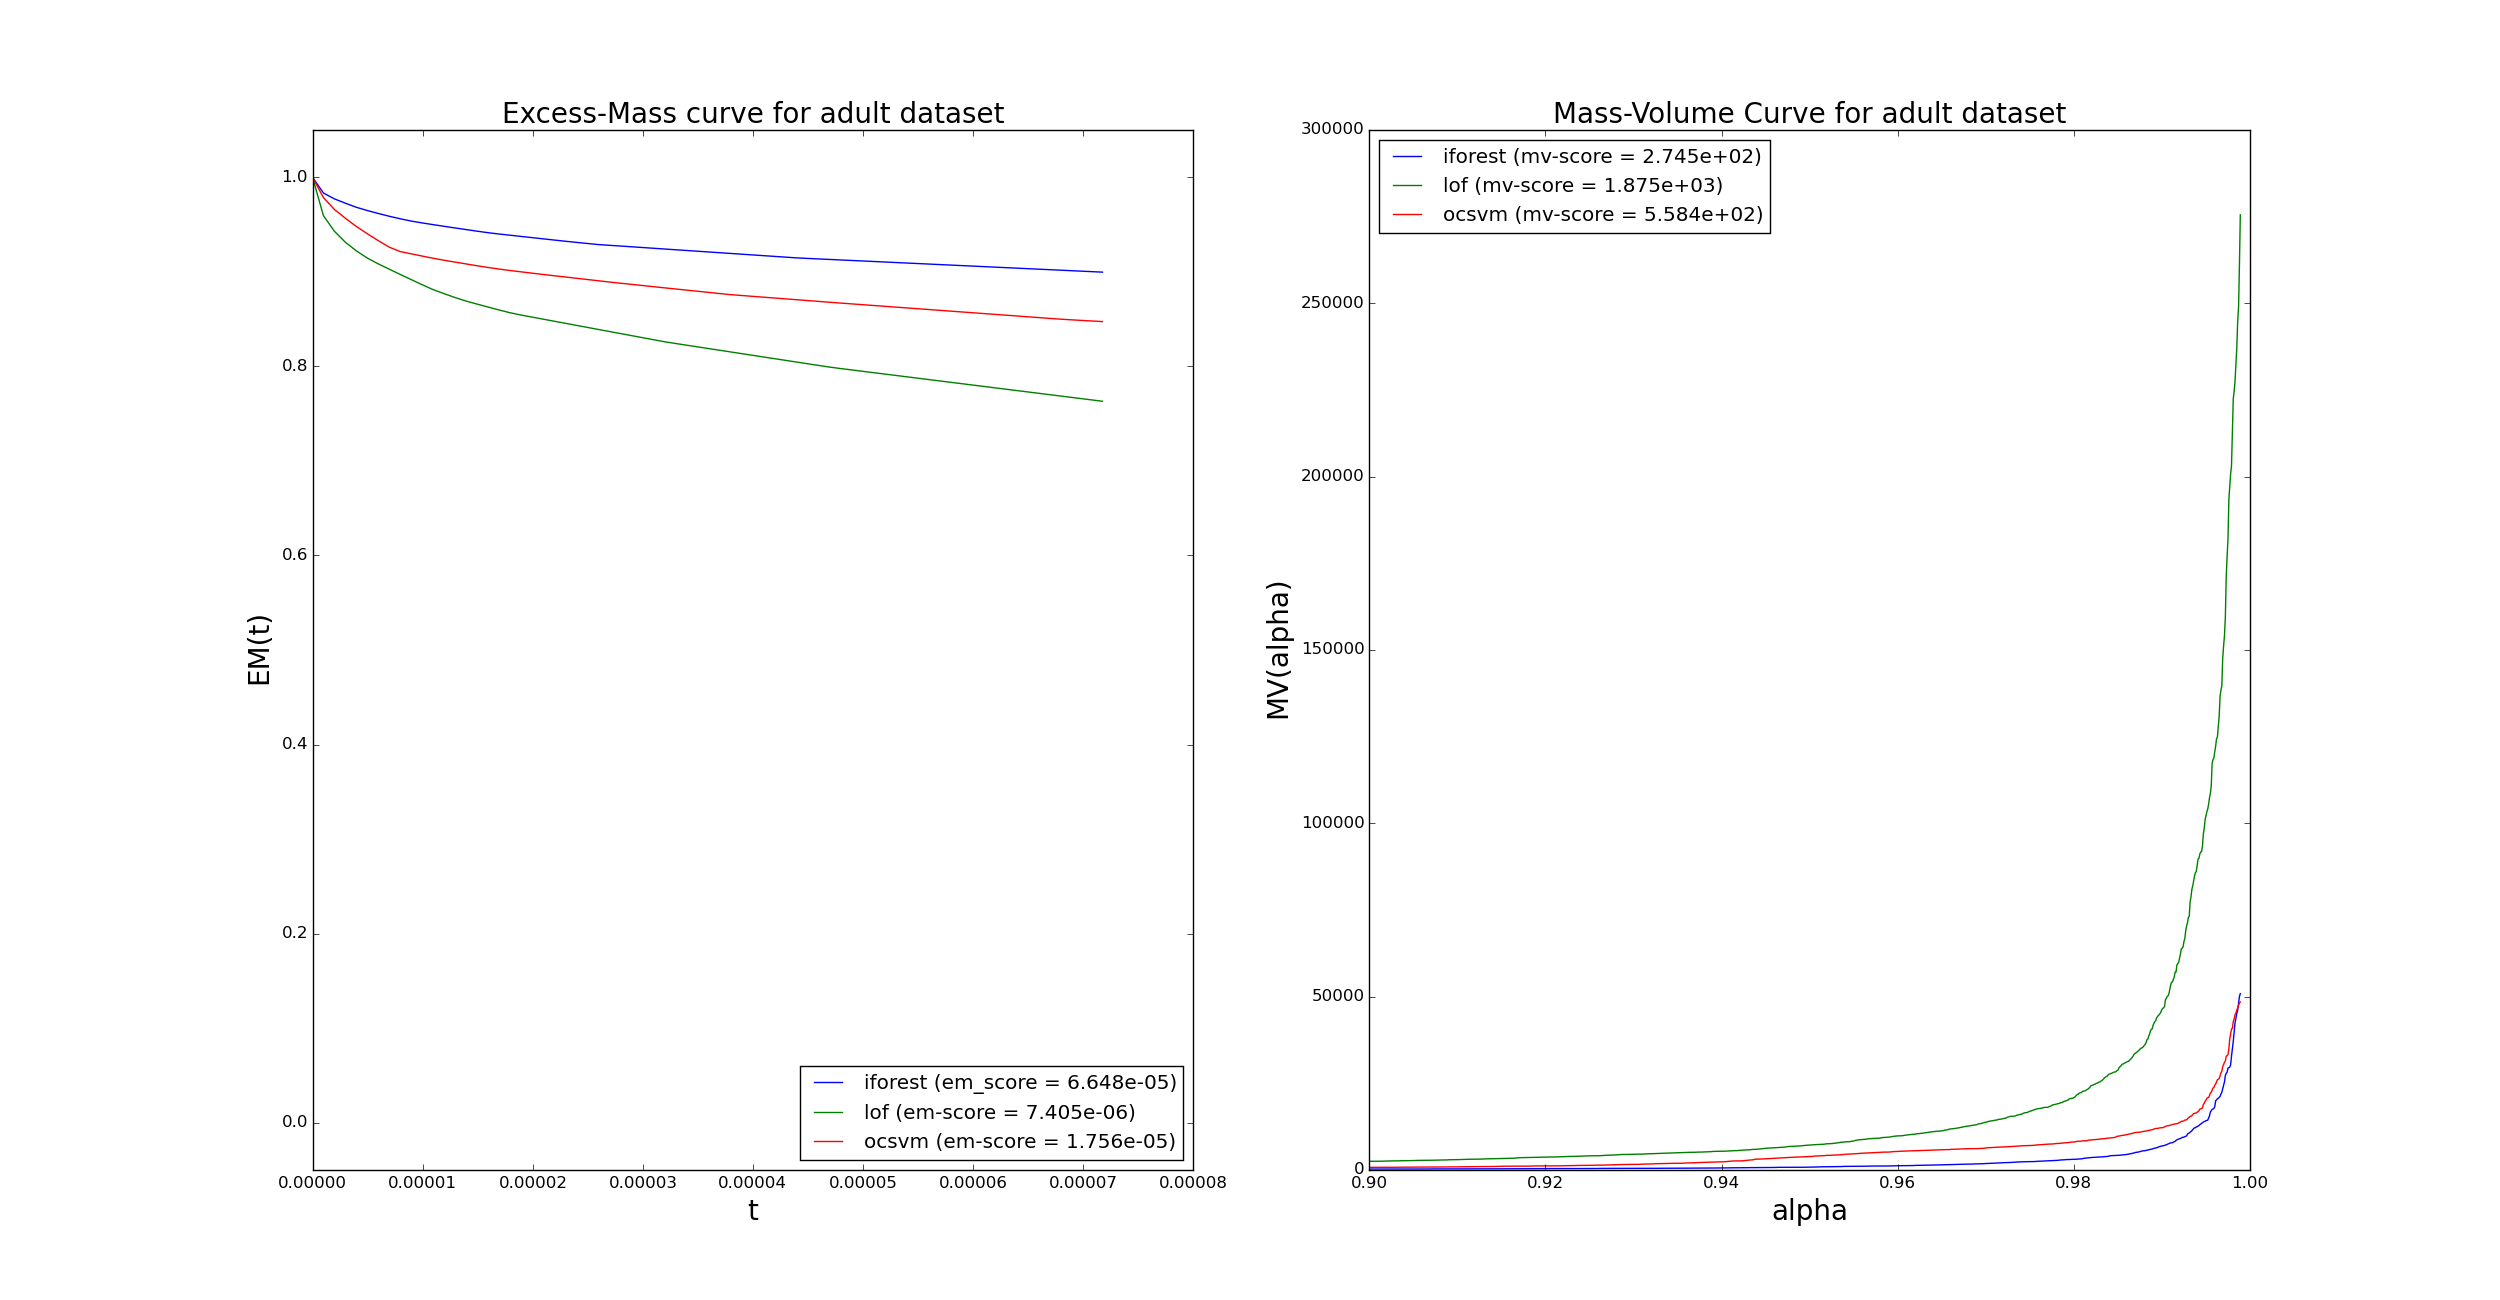
\includegraphics[trim=172 52 165 70, clip, width=\linewidth]{fig_source/evaluation_fig/mv_em_adult_unsupervised_09_factorized.png}
\label{evaluation:mv_em_adult_unsupervised}
\end{figure}
